\documentclass[a4paper]{article}

\usepackage{amsmath}
\usepackage{amssymb}
\usepackage{stellar}
\usepackage{parskip}
\usepackage{fullpage}
\usepackage{stellar}
\usepackage{wrapfig}
\usepackage{tikz}
\usepackage{wasysym}
\usepackage{stackengine,scalerel}
\stackMath
\def\trianglelefteqslant{\ThisStyle{\mathrel{%
  \stackinset{r}{.75pt+.15\LMpt}{t}{.1\LMpt}{\rule{.3pt}{1.1\LMex+.2ex}}{\SavedStyle\leqslant}%
}}}

\usetikzlibrary{arrows}
\usetikzlibrary{decorations.pathreplacing}

\title{Analisi I}
\author{Paolo Bettelini}
\date{}

\begin{document}

\maketitle
\tableofcontents

\pagebreak

\section{Sottoinsiemi finali}

\sdefinition{Sottoinsieme finale}{
    Un sottoinsieme \(E \subseteq \mathbb{N}\) si dice \textit{finale} se
    \(E=\{n_0, n_0+1, n_0+2, \cdots\}\)
    per qualche \(n_0 \in \mathbb{N}\).
}

Esiste quindi un valore \(n\in \mathbb{N}\) tale che
\[
    E= \{ n \in \mathbb{N} \,|\, n \geq n_0 \}
\]

\sproposition{}{
    Usando l'assioma indutivo si deduce che se \(A\) è un insieme tale che \(n_0\in A\)
    e \(\forall n \in A, S(n) \in A\), allora \(A\) è finale.
}

\section{Combinatorica}

Il valore \(n!\) è pari alla cardinalità dell'insieme di tutte le funzioni fa \(F_n\) a \(F_n\)
che sono biettive. Dove \(F_n = \{ 1,2,3 \cdots, n \}\).
\[
    n! = \left| \left\{ f \colon F_n \to F_n \right\} \right|
\]

\sproof{Cardinalità di queste funzioni}{
    \begin{itemize}
        \item Il caso base è \(F_1\), che contiene solo 1 elemento e \(1!=1\).
        \item Caso induttivo: notiamo che dato l'insieme \(F_n\), aggiungendo un oggetto
        quest'ultimo possiamo posizionarlo in \(n+1\) posizioni. Di conseguenza, il nuovo numero di
        permutazioni è \(n!(n+1) = (n+1)!\).
    \end{itemize}    
}

La funzione \(\sigma(n)\) è una funzione di permutazione (funzione biettiva che permuta \(n\) elementi).
Infatti, le permutazione di \(n\) sono \(n!\), ossia la cardinalità, cioè tutte le funzioni biettive possibili per permutare gli oggetti.

\sdefinition{Disposizioni}{
    Le \textit{disposizioni} di \(k\) oggetti scelti fra \(n\) oggetti,
    dove \(1\leq k \leq n\), sono il numero delle funzioni
    iniettive \(f\colon F_k \to F_n\).
    \[
        D_{n,k} = \frac{n!}{(n-k)!}
    \]
}

\sdefinition{Combinazioni}{
    Le \textit{combinazioni} di \(k\) oggetti scelto fra \(n\) oggetti,
    dove \(1\leq k \leq n\), sono il numero di sottoinsiemi di \(F_n\)
    di cardinalità \(k\).
    \[
        C_{n,k} = \binom{n}{k} = \frac{n!}{k!(n-k)!}
    \]
}

Abbimao che
\[
    D_{n,k} = k! \cdot C_{n,k}
\]

\slemma{Proprietà dei coefficienti binomiali}{
    Per ogni \(0 \leq k \leq n\)
    \[
        \binom{n}{k} = \binom{n}{n-k}
    \]
}

\pagebreak

\stheorem{Leggi di De Morgan}{
    \[
        {(A \cap B)}^c = A^c \cup B^c
    \]
    e
    \[
        {(A \cup B)}^c = A^c \cap B^c
    \]
    con il complementare rispetto a qualche insieme \(X\).
}

\sproof{Leggi di De Morgan}{
    \(x\in {(A \cap B)}^c\) è equivalente a  \(x \notin A \cap B\),
    che è equivalente a \(x\notin A\) o \(x\notin B\).
    Allora \(x\in A^c\) o \(x\in B^c\), e quindi \(x \in A^c \cup B^c\).
}

\stheorem{Teorema del binomio}{
    Let \(n \in \mathbb{N}\) and \(x,y \in \mathbb{R}\).
    \[
        {(x+y)}^n = \sum_{k=0}^n \binom{n}{k} x^{n-k}y^k
    \]
}

\subsection{Funzione indicatrice}

\sdefinition{Funzione indicatrice}{
    Sia \(X\) un insieme e \(E \subseteq X\). La \textit{funzione caratteristica}
    di \(E\) è data da
    \[
        1_E = \begin{cases}
            1 & x \in E \\
            0 & x \notin E
        \end{cases}
    \]
}

Dati due insiemi \(E\) e \(F\), abbiamo \(E \neq F \implies 1_E \neq 1_F\).

%TODOURGENT mettere in abstract algebra
%La composizione di funzione è un operazione binaria in x^x.
La notazione \(y^x\) indica \(\{ f\colon x \to y \}\), cioè tutte le funzioni da \(x\) a \(y\).

La funzione \(\Xi \colon \mathcal{P}(X) \to {\{ 0,1 \}}^X\)
è biettiva. La funzione \(f\colon X \to \{0,1\}\) è pari a \(f=1_E\) per
\(E = \{ x \,|\, f(x)=1 \}\).
Una funzione che ti dice \(1\) se l'elemento sta nel sottoinsieme, 0 altrimenti.
Quindi \[ |\mathcal{P}(X)| = |{\{0,1\}}^X| = 2^n \]

\subsection{Altre proprietà}

\[
    \sum_{k=0}^n \binom{n}{k}\cdot {(-1)}^k = 0
\]
Questa è la somma dei sottoinsiemi con un numero pari di elementi meno quelli con un numero dispari.

\pagebreak

\section{Interi relativi}

In \(\mathbb{N}\) è definita la funzione \(+\colon {\mathbb{N}}^2 \to \mathbb{N}\)
dove \((m,n) \to m+n\).

Abbiamo chiaramente che \((a,b) = (a', b') \iff a=a' \land b=b'\).

Le prorpietà sono:
\begin{itemize}
    \item è associativa;
    \item è distributiva;
    \item esiste un elemento neutro \(0\) tale che \(m+0=m, \forall m \in \mathbb{N}\)
\end{itemize}

Tuttavia, \(m-n\) è definito solo per \(m \geq n\).
%Per costruire gli interi \(\mathbb{Z}\) da \(\mathbb{N}\) si definisce la sottrazione prendendo
%le coppie \((m,n) ~ (m',n')\)
%se e solo se \(m+n' = m' + n\). Allora \(m-n = m'-n'\).
%Abbiamo quindi, per esempio, che \(-1 \equiv (0,1)\).

Definiamo \(\mathbb{Z}\) come l'insieme 
\[
    \mathbb{Z} = \{ 0, \pm 1, \pm 2, \pm 3, \cdots \}
\]
Abbiamo allora \(\forall n \in \mathbb{Z}, \exists_{=1} n'=-n \,|\, n+(-n) = 0\),
e quindi
\[
    n-m \triangleq n + (-m)
\]
Abbiamo quindi la somma \(+\colon {\mathbb{Z}}^2 \to \mathbb{Z}\)
che gode di tutte le proprietà precedenti ma in più 
\[
    \forall n \in \mathbb{Z}, \exists -n \,|\, n+(-n) = 0
\]

Per definire gli inversi di tutti i numeri \(\neq 0\), si introducono le frazioni \(\frac{m}{n}\)
con \(m\in\mathbb{Z}\) e \(n\in{\mathbb{N}}^+\).

Si dice che due frazioni sono equivalenti \(\frac{m'}{n'}\) e \(\frac{m}{n}\)
se \(mn' = m'n\).
I numeri razionali sono descritti dalle frazioni quando si identificano
con frazioni equivalenti (classe di equivalenza), e le operazioni vengono fatte sulle frazioni.
La classe di equivalenza è quindi data relazione \(\frac{m}{n} \sim \frac{m'}{n'} \iff mn'=m'n\).

Abbiamo che
\[
    \frac{m}{n} \cdot \frac{p}{q} \to \frac{mq+pn}{nq}
\]

Risulta che i razionali \(\mathbb{Q}\) con le operazioni \(+\) e \(\cdot\) introdotte.
Quindi \((\mathbb{Q}, +)\) è un gruppo abeliano, \(({\mathbb{Q}}^*, \cdot)\) è anch'esso un gruppo abeliano
(da notare l'assenza dello 0).

Vale la proprietà distributiva di prodotto rispetto alla somma
\[ r\cdot (s+t) = r\cdot s + r\cdot t \]

Quindi \((\mathbb{Q}, +, \cdot)\) è un campo, per cui possiede le operazioni \(+\) e \(\cdot\)
con le prorpietà alle quali siamo abituati.

\pagebreak

In particolare, in \(\mathbb{Q}\) si possono risolvere le equazioni di primo grado.
\[
    ax+b=0
\]
con \(a,b,x\in\mathbb{Q}\), \(x\neq 0\).
\begin{align*}
    ax+b+(-b)&=-b \\
    ax&= -b \\
    a^{-1}(ax) &= -a^{-1}b \\
    a^{-1}ax &= -a^{-1}b \\
    x &= -\frac{b}{a} 
\end{align*}

Il campo di \(\mathbb{Q}\) ha un ordinamento totale dove \(r \leq s\) se e solo se \(r - s\) è
non-negativa.

In \(\mathbb{Q}\) è definito un ordinamento che è compatibile ocn le operazioni \(+\) e \(\cdot\),
cioè soddisfa le condizioni
\begin{align*}
    r \leq s \implies t + r \leq t + s \\
\end{align*}
con \(t\in \mathbb{Q}\) e con \(t \geq 0\) abbiamo \(tr \leq ts\).

\sdefinition{Campo ordinato}{
    Un campo \(F\) nel quale è definito un ordinamento per il quale valgono le proprietà
    appena date, viene detto \textit{ordinato}.
}

Non tutte le equazioni in \(\mathbb{Q}\) sono risolvibili.

\stheorem{Radice di due}{
    L'equazione \[ x^2 = 2 \] non ha soluzioni in \(\mathbb{Q}\).
}

\sproof{Radice di due}{
    Supponiamo che esista una frazione ridotta ai minimi termini \(r = \frac{m}{n}\),
    tale che \(r^2 = 2\). Abbiamo quindi che \(\frac{m^2}{n^2} = 2\), quindi \(m^2 = 2n^2\).
    Ciô ci dice che \(m^2\) è pari. Allora, \(2\) è un fattore anche di \(m\) (siccome la fattorizazzione è unica e non cambia),
    quindi \(m\) è pari. Di conseguenza, se \(m\) è divisibile per \(2\), allora \(m^2\) è divisibile per \(4\).
    Abbiamo quindi \(4k=n^2\) e quindi \(n^2\) è divisibile per \(2\), anche \(n\),
    contro l'ipotesi del fatto che i due numeri fossero coprimi.
}

\pagebreak 

\section{Definizioni con ordini}

Sia \(E \subseteq X\) un insieme dove \(E \neq \emptyset\).

Si dice che \(m\in X\) è \textit{maggiorante} di \(E\) se \(\forall x \in E, x \leq m\). \\
Se un tale valore esiste, \(E\) si dice \textit{superiormente limitato}.

Si dice che \(m\in X\) è \textit{minorante} di \(E\) se \(\forall x \in E, x \geq m\). \\
Se un tale valore esiste, \(E\) si dice \textit{inferiormente limitato}.

L'insieme \(E\) si dice \textit{limitato} se è limitato sia inferiormente che superiormente.

Un valore \(m\in X\) si dice \textit{massimo} di \(E\) se \(M\) è un maggiorante di \(E\) e \(m\in E\). \\
Un valore \(m\in X\) si dice \textit{minimo} di \(E\) se \(M\) è un minorante di \(E\) e \(m\in E\).

\subsection{Considerazioni}

Nel caso in cui l'insieme \(E\) sia finito, vi è un massimo ed un minimo.
Tuttavia, in caso contrario, valori massimi e minimi non esistono necessariamente.

Consideriamo per esempio \(X=\mathbb{Q}\) ed
\[
    E = \left\{ r_n = \frac{n-1}{n}, \quad n\in{\mathbb{N}}^* \right\}
\]
Possiamo notare che il valore \(0\) è il minimo di \(E\).
Vi sono diversi minoranti di \(E\), come \(-1\), \(-30\) etc. In generale, tutti i \(x\leq 0\) sono
dei minoranti di \(E\).
I maggioranti di \(E\) sono tutti i valori \( x \geq 1\).

Tuttavia, non vi è un massimo. Per dimostrarlo prendiamo \(r_n \in E\).
È facile vedere che \(r_n\) non può essere maggiorante in quando se \(n'>n\), \(r_{n'}>r_n\).
Dato qualsiasi \(r_n\), è possibile trovare un altro elemento in \(E\) che è maggiore, e per cui non
esistono maggioranti.

Notiamo che il numero \(1\), che è il maggiorante, è infatti il più piccolo dei maggioranti:
supponiamo che \(z<1\), verifichiamo quindi che \(z\) non è un maggiorante.
Il valore \(z\) non è maggiorante di \(E\) se esiste una \(x \in E\) tale che \(x > z\).
Esiste infatti \(n\) tale che \(r_n > z\), studiamo quindi la disequazione
\begin{align*}
    r_n - z = 1 - \frac{1}{n} - z = (1-z) - \frac{1}{n} > 0
\end{align*}
purché \(1-z>1\). Qualcunque numero più piccolo di \(z\) sia dato, si possono fare
altri valori maggiori, dati quindi da
\[
    n > \frac{1}{1-z}
\]

\pagebreak

\subsection{Estremi superiori e inferiori}

\sdefinition{Estremo superiore}{
    Sia \(E \subseteq X\) un sottoinsieme non-vuoto, diciamo che \(\mu\) è
    l'\textit{estremo superiore} di \(E\) se \(\mu\) è un maggiorante di \(E\) e
    \(\mu\) è il più piccolo del maggioranti.
    Scriviamo quindi
    \[
        \mu = \sup E
    \]
}

\sdefinition{Estremo inferiore}{
    Sia \(E \subseteq X\) un sottoinsieme non-vuoto, diciamo che \(\mu\) è
    l'\textit{estremo inferiore} di \(E\) se \(\mu\) è un minorante di \(E\) e
    \(\mu\) è il più grande del minoranti.
    Scriviamo quindi
    \[
        \mu = \inf E
    \]
}

I valori di minimo, massimo, estremo inferiore, estremo superiore, sono unici se esistono.
Ci sono sottoinsiemi di \(\mathbb{Q}\) che non hanno estremi superiori (e quindi ci sono tante funzioni senza limiti, derivate e integrali.
L'analisi in \(\mathbb{Q}\) sarebbe quindi un disastro per questo motivo).

\stheorem{}{
    Sia
    \[
        E = \left\{ r \in \mathbb{Q} \,|\, r \geq 0 \land r^2 \leq 2 \right\}
    \]
    allora, \(E\) è non-vuoto, limitato superiormente, ma non esiste il suo estremo superiore.
}

\sproof{}{
    \begin{itemize}
        \item Per dimostrare che \(E \neq \emptyset\) possiamo semplicemente darne un elemento, come
        per esempio \(1\).
        \item L'insieme \(E\) è banalmente limitato superiormente
            da tutti i valori \(x \geq 2\). 
        \item Supponiamo per assurdo che esista un \(\mu = \sup E\). Notiamo che ovviamente \(\mu >0\).
        Possiamo notare che \(\mu^2 = 2\) è impossibile per il teorema di Euclide. Allora, \(\mu\)
        potrebbe essere minore di 2 oppure maggiore di 2.
        Supponiamo che \(\mu^2 < 2\), allora dimostro che \(\exists x \in E\) tale che \(x > \mu\)
        e quindi che \(\mu\) non è maggiorante.
        Consideriamo quindi i numeri razionali della forma
        \[
            \mu + \frac{1}{n}
        \]
        che sono chiaramente più grandi di \(\mu\).
        Possiamo quindi scegliere \(n\) sufficientemente grande tale che \({(\mu + \frac{1}{n})}^2 < 2\),
        e quindi \(\mu + \frac{1}{n} \in E\) in quanto
        \begin{align*}
            2 - {\left(\mu + \frac{1}{n}\right)}^2 &= 2 - \mu^2 + \frac{2\mu}{n} + \frac{1}{n^2} \\
            &= (2-\mu^2) - \frac{2\mu}{n} - \frac{1}{n^2}
        \end{align*}
        è chiaramente più grande di \((2-\mu^2) - \frac{2\mu}{n} - \frac{1}{n}\).
        Ciò è dato dal fatto che \(\frac{1}{n} > \frac{1}{n^2}\).
        \[
            \frac{2\mu + 1}{n} < 2-\mu^2, \quad n > \frac{2-\mu^2}{2\mu + 1}
        \]
        Analogamente, si dimostra che \(\mu^2\) non può essere nemmeno maggiore di \(2\),
        e quindi \(\mu\) non esiste.
    \end{itemize}
}

\pagebreak

È facile verificare che inf, sup, min, max se esistono sono unici.
Se esiste il massimo di \(E\), allora esiste il \(\sup E\) e coincidono.
Infatti, il massimo esiste se esiste \(\sup E\) e \(\sup E \in E\).

In \(\mathbb{Q}\) (e poi in \(\mathbb{R}\)), se \(E\) non è limitato superiormente (cioè non ha maggiornate
cioè \(\forall M \in \mathbb{Q}, \exists e \in E\) tale che \(e > M\)) si dice che
\[
    \sup E = +\infty
\]
Analogamente se \(E\) non è limitato inferiormente si dice che
\[
    \inf E = -\infty
\]

Possiamo quindi notare che
\[
    \sup \emptyset = -\infty
\]
e
\[
    \inf \emptyset = +\infty
\]

\sdefinition{Numeri reali}{
    Definiamo \(\mathbb{R}\) come un campo totalmente ordinato nel quale
    vale la seguente proprietà del \(\sup\):
    \[
        \forall E \subseteq \mathbb{R}, \quad E \neq \emptyset \land E \text{ limitato sup. esiste}
    \]
}

Bisogna tuttavia dimostrare l'unicità di questa costruzione e la sua esistenza.

\stheorem{Teorema di unicità}{
    Siano \(F_1\) e \(F_2\) due campi ordinati nei quali
    vale la proprietà del sup di prima. Allora, esiste una biezione
    \(\phi\colon F_1 \to F_2\) tale che è un isomorfismo del gruppo additivo
    \(\phi(x+_{F_1}y) = \phi(x) +_{F_2} \phi(y)\) per ogni \(x,y\in F_1\)
    e \(\phi(-x) = -\phi(x)\) per ogni \(x\in F_1\).
    % che si possono scrivere anche in un modo solo.
    Se aggiungiamo anche che \(\phi(x \cdot_{F_1} y) = \phi(x) \cdot_{F_2} \phi(y)\)
    per tutte le \(x,y \in F_1\) e \(\phi(x^{-1}) = {\phi(x)}^{-1}\)
    abbiamo un isomorfismo di campo.
    Se aggiungiamo anche che \(x \leq y \iff \phi(x) \leq \phi(y)\), abbiamo quindi un isomorfismo
    di campo ordinato.
}

Date le proprietà di un campo, ogni campo genera un insieme dei razionali \(\mathbb{Q}\).
Chiaramente, diversi campi generano \(\mathbb{Q}\) diversi ma con gli stessi elementi in un certo senso.
Possiamo mappare un insieme dei razionali di un campo a quello di un altro.

È facile definire \(\phi_0\colon \mathbb{Q}_1 \subseteq F_1 \to \mathbb{Q}_2 \subseteq F_2\).
Usando la proprietà del sup possiamo eseguire tale mappatura.
Dato \(x\in F_1\), abbiamo \(x = \sup \{ r \in \mathbb{Q}_1 \,|\, r \leq x \} = \sup E_x\).
Allora \(\phi (x) = \sup \{ \phi_0(r) \,|\, r \in E_x \}\).
Così viene esteso \(\phi\) a tutto. Bisognerebbe tuttavia dimostrare che le proprietà classiche vengano
preservate.

Per dimostrare l'esistenza è necessario considerare
\[\mathbb{R} = \{ \text{ numeri decimali } n, a_1, a_2, a_3, \cdots \} \text{ finiti o infiniti periodici o meno }\]
dove \(a_k \in \{0,1,2,3,4,5,6,7,8,9\}\).

Con la prescrizione che \(n,a_1, a_2, a_3, \cdots, a_k, \overline{9} = n, a_1, \cdots, a_{k-1}, (a_k+1)\).

I numeri reali possono essere anche definiti mediante le sezioni di Dedekind.
Alternativamente si possono definire mediante le successioni di Cauchy.

\paragraph{Definizione di somma e prodotto:}

Prendiamo \(x = n,a_1,\cdots,a_k\cdots\) e \(y = m,b_1,\cdots,b_k\cdots\)
che sono due numeri decimali, nessuno dei quali con period \(9\),
allora
\[
    x=y \iff n=m \land a_k=b_k
\]
e
\[
    x<y \iff n < m \lor (n=m \land a_i = b_i, i < k \land a_k < b_k)
\]

Le operazioni sono definite mediante troncamenti.
Verificiamo che questo modello di \(\mathbb{R}\) soddisfi la proprietà del sup.

Prendiamo quindi  \(E\subseteq \mathbb{R}\) non vuoto e sup limitato. Costruiamo
il sup mediante un algoritmo.
\[
    \sup E = \mu = n,a_1,a_2,a_3,\cdots,a_k,\cdot
\]
Per ogni \(x\in E\) scriveremo \(n_x,a(x)_1, a(x)_2,\cdots\).
\(E\) è non-vuoto e limitato sup, per cui
\[
    \{ n_x \,|\, x\in E \}
\]
è un insieme di numeri in \(\mathbb{Z}\) limitato superiormente.
Sia
\[
    N = \max\{ n_x \colon x \in E \}
\]
Prendiamo ora tutti gli insiemi
\[
    E_0 = \{ x\in E \,|\, n_x = N \} \neq \emptyset
\]
Poniamo \(a_1 = \max \{ a(x)_1 \,|\, x \in E_0 \}\)
Abbiamo quindi
\[
    E_1 = \{ x \in E_0 \,|\, a(x)_1 = a_1 \} \neq \emptyset
\]
Poniamo ora \(a_2 = \max \{ a(x)_2 \,|\, x \in E_1 \}\).
Con lo stesso metodo troviamo \(a_3, a_4, \cdots\), ossia
\[
    a_k = \max \{ a(x)_k \,|\, x \in E_{k-1} \} \quad a_{k+1} = \max\{ a(x)_{k+1} \,|\, x \in E_k \}
\]
Trovando quindi
\[
    \mu = N,a_1,a_2,\cdots
\]

Dico che \(\mu\) è un maggiorante di \(E\), e che se \(z<\mu\), \(z\) non è maggiorante.
Sia allora \(\overline{x} \in E\), quindi
\[
    \overline{x} = n_{\overline{x}}, a(\overline{x})_1, a(\overline{x})_2, \cdots
\]
Allora \(n_{\overline{x}}\leq N\) se \(n_{\overline{x}} < N\). \(\overline{x} < \mu\).
Gli elementi in \(E_0\) sono al massimo \(a_1\).
Se \(n_{\overline{x}} = N\) e \(n_{\overline{x}} \in E_0\) e \(a_1(\overline{x}) = a_1\). \\
Se \(a(\overline{x})_1 < a_1 \implies \overline{x} < \mu\).\\
Se invece \(a(\overline{x})_1=a_1 \implies \overline{x} \in E_1\) e \(a(\overline{x})_2 \leq a_2\) \\
Fino che ad un certo punto non trovo un decimale diverso.

Iterando, se \(\exists k\) tale che \(a(\overline{x})_k < a_k \implies \overline{x} < \mu\).
Se \(\forall k, a(\overline{x})_k = a_k\), allora \(\overline{x} = \mu\) e \(\mu\) è il max di \(E\).
Questo procedimento non dimostra che \(\mu \in E\).

Mostriamo ora che è il più piccolo dei maggioranti. Sia
\[
    z = n_z, a(z)_1, a(z)_2, \cdots < \mu
\]
Deve quindi succedere che o \(n_z < N\), e allora \(\forall x\in E_0 \neq \emptyset, z<x\),
oppure \(n_z = N\) e \(a(z)_j = a_j\) per tutte le \(j<k\) ma \(a(z)_k < a_k\).
Allora \(\mu = \sup E\).

\subsection{Conseguenze della proprietà del sup}

Le conseguenze della prorpietà del sup sono:
\begin{itemize}
    \item \textbf{proprietà archimedea:} \(\forall x \in \mathbb{R}, \forall a > 0, \exists n\in\mathbb{N} \,|\, na>x\) (in realtà vale anche in \(\mathbb{Q}\)).
    \item \textbf{densità dei razionali nel reali:} \(\forall x,y \in \mathbb{R}\) dove \(x<y\), esiste \(r\in\mathbb{Q}\,|\, x<r<y\).
\end{itemize}

\stheorem{Esistenza delle radici nei reali}{
    \[
        \forall y>0, \forall n \in \mathbb{N}, n \geq 1,
        \exists_{=1} x>0 \,|\, x^n = y
    \]
}

\sproof{}{
    Sia \[ E = \{ z \in \mathbb{R} \,|\, z>0 \land z^n \leq y \} \]
    Dobbiamo quindi mostrare che \(E\) non è vuoto, ed è limitato superiormente.
    Definiamo \(x = \sup E\) e mostriamo che \(x^n = y\).
    \begin{itemize}
        \item \textbf{Non vuoto:} se \(y \geq 1\), basta scegliere \(x=1\) in quanto \(x^n=1 \leq y\).
        Altrimenti, se \(y < 1\), poniamo \(x=y\) e notiamo che, perché \(y < 1\), allora
        \(y^n < y\), e quindi \(y \in E\).
        \item \textbf{Limitato superiormente:} \(E\) è limitato superiormente, infatti \(1+y\)
        è un maggiorante di \(E\). Se \(z \geq (1+y)\), poiché la funzione \(t\to t^2\) è crescente per \(t > 0\),
        si ha \(z^n \geq {(1+y)}^n > {(1+y)} > y \implies z \notin E\).
        Sia \(x =\sup E\). Dico che \(x^n = y\). Dimostro che se suppongo \(x^n > y\)
        allora per \(k\) grande
        \[
            {\left(x- \frac{1}{k}\right)}^n > y
        \]
        e quindi \(x-\frac{1}{k}\) è ancora un maggiorante di \(E\), contro l'ipotesi impossibile
        perché \(x\), che è il \(\sup E\), è il più piccolo maggiorante.
        Invece, se \(x^n < y\) allora per \(k\) grande
        \[
            {\left(x + \frac{1}{k}\right)}^n < y
        \]
        allora \(x+\frac{1}{k}\in E\) ed è più grande di \(x\), e \(x\) non è quindi un maggiorante (assurdo).
        Visto che \(x\) non può essere nè più grande nè più piccolo, \(x^n=y\).
        \item \textbf{Unicità:} notiamo che se \(0 < t_1 < t_2 \implies t_1^n < t_2^n\).
    \end{itemize}
}

Possiamo anche mettere \(z\geq 0\) così dimostrare che \(E\neq \emptyset\) è più facile.

Esercizio: dimostrazione per induzione che \(0<y<1 \implies y^n < y\), per \(n > 1\).
(Che abbiamo usato nell'ultima dimostrazione).

\subsection{Esercizi sup}

\sexercise{}{
    Let
    \[
        E = \left\{ x\in\mathbb{R} \,|\, \frac{1}{2} \leq x < 5 \right\}
    \]
    and the sequence \[
        F = \{ x = x_n \,|\, x_n = \frac{n + 1}{n + 2}, \quad n\in\mathbb{N}^* \}
    \]
    %%%%%%%
    Trova inf, sup, min, max (se esistono) di \(E\), \(F\), \(E \cup F\) e \(E\cap F\).
    \begin{itemize}
        \item \(E\) è limitato superiormente e inferiormente.
        Il minimo è \(\frac{1}{2}\), mentre \(5\) è un maggiorante, è il più piccolo
        dei maggioranti quindi \(\sup E = 5\), ma non vi è un massimo.
        \item \(F\) è limitato superiormente in quanto 
        \[
            x_n = \frac{n+1}{n+2} < \frac{n+2}{n+2}  =1
        \]
        È limitato inferiormente perché \(x_n > 0\).
        Per verificare sup e inf, è comodo riscrivere \[
            x_n = 1 - \frac{1}{n+2}
        \]
        Il temrine \(n+2\) cresce con \(n\), quindi \(\frac{1}{n+2}\) decresce al crescere di \(n\)
        e quindi \(x_n\) cresce approcciando \(1\). Allora con \(n=1\) il termine assume il valore più piccolo,
        ossia \(\frac{2}{3}\), quindi il minimo di \(F\). Allora siccome ci avviciamo arbitrariamente a
        \(1\), è lecito ipotizzare \(\sup F = 1\).
        Il massimo di \(F\) non esiste.
        Rimane da far vedere che se \(z < 1\) allora \(z\) non è maggiorante di \(F\)
        cioè
        \[
            x_n - z = (1-z) - \frac{1}{n+2} > 0
        \]
        purché \(\frac{1}{n+2} < 1-z\) cioè \(n > \frac{1}{1-z}-2\).
        Quindi \(z\) non è maggiorante e \(\sup E = 1\).
        \item Verificare che \(\sup (E \cup F) = \max \{ \sup E,\sup F \}\).
        Abbiamo che \(\sup E \leq \sup F\).
        In sup è il massimo dei due in quanto uno è maggiore dell'altro,
        e fa parte dell'insieme, quindi \(\sup E \cup F = 5\).
        Tuttavia, il max non esiste in quando \(5\notin  E \cup F\).
        Analogamente, \(\inf E \cup F = \frac{1}{2}\). Questo valore è anchde il minimo
        in quanto fa parte dell'insieme.
        \item Mostrare con un esempio che non c'è qualcosa di analogo per l'intersezione.
        \[
            E \cap F = \left\{ x_n = \frac{x+1}{x+2} \ \middle|\ \frac{1}{2} \leq \frac{x+1}{x+2} \leq 5 \right\}
        \]
        Quindi \(F \subseteq E\). Consideriamo allora \(E_1 = [\frac{4}{5}, 5)\)
        \[
            E_1 \cap F = \left\{ x_n = \frac{x+1}{x+2} \ \middle|\ \frac{4}{5} \leq x_n \leq 5 \right\}
        \]
        Per quali \(n\) vale che \(\frac{4}{5} \leq \frac{x+1}{x+2} = x_n\)?
        Abbiamo \(4(n+2) \leq 5(n+1)\) e quindi \(n \geq 3\).
        Allora \(\sup E_1 \cap F = 1\) e non vi è massimo, mentre \(\inf E_1 \cap F = \frac{4}{5}\)
        che è anche il minimo.
        \item Posto \(E+F = \{ x + y \,|\, x \in E, y \in F \}\)
        mostrare \(\sup E + F = \sup E + \sup F\). Supponiamo quindi che \(\sup E\) e \(\sup F\)
        siano finiti. Siccome, per definizione, \(\forall e \in E, e \leq \sup E\)
        e \(\forall f \in F, f \leq \sup F\), abbiamo che \[\forall e \in E, \forall f\in F, e + f \leq \sup E + \sup F\]
        Per mostrare che questo è il più piccolo dei maggioranti, è comodo riscrivere la definizione di
        sup dicendo che \(\mu\) è pari a \(\sup E\) se:
        \begin{enumerate}
            \item \(\forall x \in E, x\leq \mu\);
            \item \(\forall \varepsilon > 0, \mu - \varepsilon\) non è maggiorante.
        \end{enumerate}
        \textbf{Nota:} se \(x < \mu\) allora posto \(\varepsilon = \mu - x\) risulta \(x = \mu - \varepsilon\).
        Allora sia \(\varepsilon > 0\). Diciamo che esistono \(e_1\in E\) e \(f_1\in F\) tali che
        \(e_1 + f_1 > \sup E + \sup F - \varepsilon\).
        Poiché \(\sup E\) è, appunto, il supremum, esiste per definizione una \(e_1 \in E\) tale che
        \(e_1 > e_1 > \sup E . \frac{\varepsilon}{2}\).
        Analogamente, esiste \(f_1 \in F\) tale che \(f_1 > \sup F - \frac{\varepsilon}{2}\).
        Da cui \(e_1 + f_2 > \sup E - \frac{\varepsilon}{2} + \sup F - \frac{\varepsilon}{2} = \sup E + \sup F - \varepsilon\).
        \item Posto \(-E = \{ -x \,|\, x \in E\}\) mostrare che
        \(\sup -E = -\inf E\) e \(\inf -E = -\sup E\).
    \end{itemize}
}

Dimostrare che il max esiste se e solo se \(\sup E\) è finito e appartiene a \(E\).
Analogamente per il min.

\pagebreak

\sexercise{}{
    Trovare sup, inf, min, max dell'insieme
    \[
        E = \left\{ x_n = \frac{n-7}{x^2 + 1} \ \middle|\ n \geq 1 \right\}
    \]
    Questa successione ha sicuramente un minimo in quanto ci sono solamente \(6\) numeri negativi.
    Possiamo notare che il denominatore cresce più velocemente del numeratore.

    Studiamo quindi per quali indici vale \(x_n \leq x_{n+1}\). Otteniamo quindi
    \begin{align*}
        \frac{n-7}{n^2 + 1} &\leq \frac{(n+1)-7}{{(n+1)}^2 + 1} \\
        \frac{(n-7)(n^2 + 2n + 2) - (n-6)(n^2+1)}{(n^2 + 1)(n^2 + 2n + 2)} &\leq 0
    \end{align*}
    Il denominatore è positivo, quindi studiamo il numeratore
    \begin{align*}
        n^2 - 13n - 8 \leq 0
    \end{align*}
    Le radici di questo polinomio sono \(n_{1,2}= \frac{13\pm\sqrt{201}}{2}\).
    Di conseguenza, l'espressione è negativa per \(\frac{13-\sqrt{201}}{2} < n < \frac{13+\sqrt{201}}{2}\).
    Notiamo che l'estremo di sinistra è negativo. Notiamo anche che \(14^2 < 201 < 15^2\),
    e quindi l'estremo di destra è compreso fra \(14\) e \(\frac{27}{2}\).
    Allora, tutte le \(n\) intere che soddisfano l'equazione sono
    \(n=13\). Ne consegue che se \(n \geq 14\), \(x_n > x_{n+1}\).
    Il maggiornate e supremum è quindi \(x_{14}\).

}

\pagebreak

\section{Esponenziali}

\subsection{Potenze ad esponente reale e esponziali e logaritmi}

Abbiamo definito le radici n-esime come
\[
    x^\frac{m}{n} \triangleq \sqrt[n]{x^m}
\]
Si dimostra inoltre che per ogni \(p\) intero positivo,
\[
    x^{\frac{x\cdot p}{n\cdot p}} = x^\frac{m}{n}
\]
La potenza \(x^r\) è quindi ben definita con \(r\in\mathbb{Q}^{> 0}\).
Successivamente, definiamo le potenze negative
\[
    x^{-r} = {(x^-1)}^r
\]
Abbiamo le consuete proprietà:
\begin{enumerate}
    \item \(\forall x>0, x^0 = 1\);
    \item \(\forall r,s\in\mathbb{Q}, x^rx^s = x^{r+s}\);
    \item \(\forall r,s\in\mathbb{Q}, {(x^r)}^s = x^{rs}\);
\end{enumerate}

Con \(r>0\) posso definire \(0^r = 0\)
e se \(r=\frac{m}{n}\) (ridotta ai minimi termini) con \(n\) dispari
posso definire \(x^\frac{m}{n}\) se \(x<0\).

\subsection{Potenze a esponente reale}

Se \(x=1\), \(\forall a\in \mathbb{R}, x^a = 1\).
Se \(x>1\) e \(r<s\), allora \(x^r < x^s\)
\[
    r = \frac{m}{p} < s = \frac{n}{p}, m < n
\]
\[
    x^r = {(\sqrt[p]{x})}^m < {(\sqrt[p]{x})}^n
\]

Definiamo quindi la potenza reale con \(a>1\) e \(x>1\)
\[
    x^a = \sup \{ x^r \,|\, r \leq a \}
\]
Estendiamo la definizione ad \(a < 0\) come
\[
    x^a = {(x^{-1})}^{-a}
\]
E infinie se \(0<x<1\)
\[
    x^a = {(x^{-1})}^{-a}
\]

\pagebreak

\subsection{Esponenziali}

Fissata una base \(a>0\) abbiamo poi l'esponenziale che è definita da \(a^x\),
\(x\in\mathbb{R}\).

Risulta che se \(a=1\), allora la funzione è sempre \(1\).
Se \(a>1\) la funzione è stretta crescente, e strettamente descrescente se \(0<a<1\).

La funzione è biettiva tra \(\mathbb{R}\) e \((0, +\infty)\), quindi è invertibile.
La funzione inversa è \(y=\log_a(x)\).

Le proprietà dei logaritmi sono analoghe a quelle degli esponenti.
\sproposition{Proprietà dei logaritmi} {
    \[
        \log_a(xy) = \log_a(x) + \log_a(y)
    \]
    \[
        \log_a(x^y) = y\log_a(x)
    \]
    \[
        \log_a(b) = \frac{\log_c(a)}{\log_c(b)}
    \]
}

% Come trovare la terza


Il passaggio da moltiplicazione e somma di logaritmi, potrebbe non avere senso
nella seconda forma.
E.g \(\ln(x(x-1))\) non is può riscrivere come \(\ln(x) + \ln(x-1)\)
perché, se sono positivi quando moltiplicati, non è detto che lo siano separatamente.

Se abbiamo \(\log_2(x^2)\), possiamo riscriverlo come \(2 \log_2|x|\).

\pagebreak

\section{Numeri complessi}

In un campo ordinato e quindi in \(\mathbb{R}\), \(x^2 \geq 0\) e vale \(x^2 = 0 \iff x=0\).
Quindi l'equazione \(x^2 = -1\) non ha soluzione in \(\mathbb{R}\).
Estendiamo il campo \(\mathbb{R}\) costruendo un campo \(\mathbb{C}\)
che contiene una immagine isomorfa di \(\mathbb{R}\) nel quale \(z^2 = -1\)
ha soluzioni.

Tuttavia, tale campo non ammette il medesimo ordinamento che avevamo.
Definiamo quindi
\[
    \mathbb{C} = \mathbb{R} \times \mathbb{R}
\]

Definiamo l'operazione di addizione
\[
    +\colon \mathbb{C} \times \mathbb{C} \to \mathbb{C}
\]
in maniera tale che
\[
    (a,b) + (c,d) \triangleq (a+c, b+d)
\]

\begin{enumerate}
    \item anche questa somma è associativa, e commutativa come in \(\mathbb{R}\);
    \item l'elemento neutro \(0\) è la coppia \(0,0\);
    \item l'opposto di \((a,b)\) è \(-(a,b)\);
\end{enumerate}

Si può rappresentare \(\mathbb{C}\) come punti nel piano.
La moltiplicazione è definita come
\[
    (a,b) \cdot (c,d) \triangleq (ac-db,ad+bc)
\]
Questo prodotto è
\begin{enumerate}
    \item è associativo;
    \item è commutativo;
    \item l'elemento \((1,0)\) è l'elemento neutro;
    \item esiste un elemento inverso
\end{enumerate}

\[
    \forall z=(a,b) \in \mathbb{C} \,|\, (a,b) \neq (0,0),
    \exists z^{-1} = \left(\frac{a}{a^2 + b^2}, \frac{-b}{a^2 + b^2}\right) \,|\,
    zz^{-1} = (1,0)
\]

Per determinare questa forma basta risolvere \(z^{-1} = (x,y)\) dove \((a,b)(x,y) = (1,0)\).

Abbiamo quindi un campo.

Adesso, notiamo che \((0,1)(0,1) = (-1, 0)\).

\subsection{Inclusione dei reali}

Ogni number \(r\in\mathbb{R}\) può essere identificato con il numero complesso \((r, 0)\).
Cosifacendo, l'applicazione \(\varphi\colon \mathbb{R} \to \mathbb{C}\)
tale che \(\varphi(a) = (a,0)\) preserva le operazioni.

Possiamo poi scrivere \(z=(a,b)\) come \(a(1,0) + b(0,1)\).
Se identifichiamo \(i=(0,1)\), possiamo scrivere
\[
    (a,b) = a+bi
\]
che viene detta forma algebrica.
Le operazioni di numeri complessi in forma algebrica si forma con le consuete regole del calcolo letterale
e l'identità \(i^2 = -1\).

\subsection{Operazioni algebriche}

\[
    \begin{cases}
        i^0=+1\\
        i^1=+i\\
        i^2=-1\\
        i^3=-i\\
    \end{cases}
    \quad
    \begin{cases}
        i^4=+1\\
        i^5=+i\\
        i^6=-1\\
        i^7=-i\\
    \end{cases}
    \quad
    \cdots
\]

Dato \(z=a+bi\), diciamo che \(\Re(z) =a\) e \(\Im(z) = b\).

\sdefinition{Coniugio}{
    Dato \(z=a+bi\in\mathbb{Z}\),
    \[
        \overline{z} = a-bi
    \]
}

Chiaramente, \(z + \overline{z} = 2\Re(z)\). Possiamo quindi dire che

\[
    \Re z = \frac{z + \overline{z}}{2}
\]
e
\[
    \Im z = \frac{z-\overline{z}}{2i}
\]

\sproposition{Proprietà del coniugio}{
    \begin{itemize}
        \item \textbf{involutivo:} \(\overline{\overline{z}} = z\);
        \item \(\overline{z+w} = \overline{z} + \overline{w}\);
        \item \(\overline{zw} = \overline{z}\cdot\overline{w}\);
        \item \(w \neq 0 \implies \overline{z^{-1}} = {\left(\overline{z}\right)}^{-1}\);
        \item \(w \neq 0 \implies \overline{\left(\frac{z}{w}\right)} = \frac{\overline{z}}{\overline{w}}\);
        \item \(\overline{z^n} = {(\overline{z})}^n\) per \(n\in\mathbb{Z}\).
    \end{itemize}
}

Per ogni numero complesso \(z\),
\[
    {|z|}^2 = z\overline{z}
\]
e per ogni numero complesso \(w\)
\[
    \overline{wz} = wz\overline{wz} = z\overline{z}w\overline{w} = |z|^2|w|^2
\]

In particolare, \(|z^n| = |z|^n\).

La disuguaglianza \(||z| - |w|| \leq |z-w|\).

\begin{itemize}
    \item \(|wz| = |w|\cdot|z|\);
    \item \(|w+z| \leq |w| + |z|\).
\end{itemize}

% Il modulo è minore o uguale all'abs reale + abs imm

Da dimostrare: \(|z+w|^2 \leq {(|z| + |w|)}^2\).

\subsection{Passaggio polari e cartesiane}

Dato \(x+iy = r(\cos\theta + i\sin\theta)\) e il punto polare \((r, \theta)\)
abbiamo
\[
    r = \sqrt{x^2 + y^2}
\]
e \[
    \theta = \arctan\left(\frac{y}{x}\right)
\]

\subsection{De Moivre}

\[
    z^n = r^n {(\cos \theta + i\sin\theta)}^n = \sum_{k=0}^n \binom{n}{k}
    i^k {(\cos\theta)}^{n-k}{(\sin\theta)}^k
\]

\section{Distanza fra due insiemi}

La distanza (minima) fra due insiemi è definita come
\[
    \text{dist}(S, R) = \inf \{ d(z,w) \,|\, z \in S \land w \in R \}
\]

\section{Teorema di Ruffini}

Dato un polinomio \(p(z)\), \(z_0\) è una radice di \(p(z)\) se esiste
un polinomio \(q(z)\) con \(\deg q(z) = \deg p(z) - 1\)
tale che \[p(z) = (z-z_0)q(z)\], cioè se \(p(z)\) è divisibile per \(z-z_0\).

La radice \(z_0\) ha moltiplicità \(m \geq 1\) se
\(p(z)\) è divisibile per \((z-z_0)^m\) ma non per \((z-z_0)^{m+1}\).

% Esercizio: dimostrare per induzione che l'enunciato del teorema fondamentale dell'algebra
% è equivalente a: Se P(z) è un polinomio di grado n \geq 1, allora P(z) ha almeno una radice.
% => è banale. <= per induzione (per Ruffini)

\pagebreak

\section{Spazi metrici}

%\sdefinition{Metrica della valle}{
%    La funzione di distanza della metrica della valle fra due punti \(a=(x,y)\) e \(b=(t,u)\)
%    è definita come
%    \[
%        d(a, b) = \begin{cases}
%            |y-u| & x = t \\
%            |y| + |x-t| + |u| & x \neq t
%        \end{cases}
%    \]
%}

%\sdefinition{Distanza in un grafo}{
%    Distanza in un grafo
%    \[
%        d(a, b) = \inf \{ \text{lunghezza dei cammini che congiungono a e b} \}
%    \]
%}

\sdefinition{Insieme aperto in spazio metrico}{
    % TODO URGENT
    Un sottoinsieme \(A \subseteq X\) è \textit{aperto} se tutti i punti sono interni in \(A\).
}

%\sproposition{Proprietà degli aperti}{
%    \begin{enumerate}
%        \item L'insieme vuoto e \(\mathbb{R}\) sono aperti;
%        \item Gli insiemi aperti in \((a,b)\), \((-\infty,b)\) e \((a,+\infty)\) sono aperti;
%        \item Data una famiglia \(\{A_i\}\) di insiemi aperti,
%        \[
%            \bigcup_{k=1}^n A_k
%        \]
%        è un insieme aperto
%        \item Se \(A_1, \cdots, A_2\) sono insiemi aperti allora
%        \[
%            \bigcap_{k=1}^n A_k
%        \]
%        è aperto.
%    \end{enumerate}
%}
%
%\sproof{Proprietà degli aperti}{
%    \begin{enumerate}
%        \item Banale
%        \item Abbiamo già verificato che se \(x\in (a,b)\), allora \((x-r,x+r) \subset (a,b)\)
%        purché \(r \leq \min\{x-a, x-b\}\)
%        \item ogni elemento dell'union appartiene ad almeno un insieme aperto, quindi se è interno
%        ad un insieme aperto la loro union è anch'essa aperta.
%        \item Siano \(A_1, \cdots, A_n\). Se l'intersezione degli \(A_i\) è vuota, allora la tesi
%        regge. In caso contrario, \(\forall k, x \in \mathbb{R}\) che è aperto quindi
%        esiste un raggio \(r > 0\) tale che la bolla di raggio attorno all'elemento è un sottinsieme di
%        tutti gli elementi di \(A_k\). Per trovare questo raggio, prendiamo il minimo di tutti
%        \[
%            r = \min\{ r_1, r_2, \cdots, r_n \}
%        \]
%        dove \(r_n\) è un raggio tale che la bolla di raggio \(r_n\) attorno all'elemento
%        è contenuta nell'insieme.
%        Se il numero degli insiemi fosse infinitio, dovremmo prendere
%        \[
%            r = \inf\{ r_1, r_2, \cdots, r_n \}
%        \]
%        che potrebbe essere anche \(0\) o non esistere.
%    \end{enumerate}
%}
%
%\sproposition{Proprietà dei chiusi}{
%    \begin{enumerate}
%        \item Se \({\{C_i\}}_{i\in I}\) è una famiglia di insiemi chiusi
%        \[
%            \bigcup_{i\in I} C_i
%        \]
%        è chiuso
%        \item Se \(C_1, \cdots, C_n\) sono intervalli chiusi,
%        \[
%            \bigcap_{i\in I} C_i
%        \]
%        è chiuso
%        \item Gli intervalli chiusi sono insiemi chiusi
%    \end{enumerate}
%}

\section{Spazi topologici}

Un punto \(x_0\) è isolato in \(E\) se \(\exists r > 0\) tale che \((x_0 - r, x_0 + r) \cap E = \{x_0\}\).

%\[
%    E = \left\{ x_n = \frac{1}{n} \,|\, n\in {\mathbb{N}}^* \right\} \cup (2,3) \cup \{4\}
%\]
%\begin{itemize}
%    \item Per ogni \(x\in (2,3)\), esiste \(r = \min\{3-x, x-2\}\)
%    dove chiaramente \((x-r, x+r) \subseteq E\)
%    \item I punti di frontiera sono \(2\), \(3\), \(4\) e tutti i punti della forma \(\frac{1}{n}\) per \(n\in {\mathbb{N}}^*\).
%    Anche \(0\) è un punto di frontiera.
%    \item I punti isolati sono quelli della forma \(\frac{1}{n}\) con \(n\in {\mathbb{N}}^*\) e \(4\).
%    \item I punti esterni sono
%    \[
%        (1,2) \cup (4,+\infty) \cup (-\infty, 0) \cup \bigcup_{n=1}^\infty \left(\frac{1}{n+1}, \frac{1}{n}\right)
%    \]
%    \item I punti di accumulazione sono
%    \([2,3] \cup \{0\} \)
%\end{itemize}

\stheorem{}{
    Sia \(E \subseteq \mathbb{R}\) (vale in qualsiasi spazio metrico)
    e sia \(x_0 \in \mathbb{R}\). Sono equivalenti:
    \begin{enumerate}
        \item \(x_0\) è di accumulazione cioè \(\forall r > 0\), \[\left((x_0-r,x_0+r) \backslash \{x_0\}\right) \cap E \neq \emptyset\]
        \item \(\forall r>0\), \((x_0 -r, x_0 + r) \cap E\) è infinito (ogni intorno contiene infiniti punti di \(E\)).
    \end{enumerate}
}

\sproof{}{
    \iffproof{
        Dimostriamo la contronominale.
        Assumiamo quindi che \(\exists r > 0\) tale che \(A=(x_0 -r, x_0 + r) \cap E\) è finito,
        e quindi \(A = \{ x_0, x_1, \cdots, x_n \}\) dove \(x_1, x_2, \cdots, x_n\)
        sono gli elementi di \((x_0 + r, x_0 - r) \cap E\) diversi da \(x_0\).
        Chiaramente, esiste un \(0 < \varepsilon < \min\{ |x_0 - x_1|, |x_0 - x_2|, \cdots, |x_0 - x_n| \}\).
        Siccome l'insieme è finito, \(\varepsilon\) esiste ed è strettamente positivo.
        Quindi, per definizione \(x_0\) non è di accumulazione.
    }{
        Trivial.
    }
}

\pagebreak

\section{Successioni}

La sequenza è limitata, limitata superiormente, limitata inferiormente,
se l'immagine è limitata, limitata superiormente, limitata inferiormente.

Diciamo che \(M=\max x_n\) se \(\forall n x_n < M\) e \(\exists n' \,|\, x_{n'} = M\).
Analogamente il min.

Definiamo inoltre \(\sup_{n} x_n = \sup \{ x_n \,|\, x \in \mathbb{N} \}\)
Analogamente per l'inf.

\sdefinition{Proprietà soddisfatta definitivamente}{
    Data una proprietà \(P\), una successione \(\{x_n\}\)
    soddisfa la proprietà \(P\) definitivamente se \(\exists N \,|\, \forall n, P(n) \geq N\).
}

Quando facciamo un limite su una successione, l'unica cosa alla quale la variabile possa
tendere è infinito.
La sequenza tende al limite superiore se dopo un certo punto il suo valore a maggiore a quello del limite,
analogamente per il limite inferiore, e entrambi per il limite in senso generale.
\[
    x_n \to l^+
\]

Possiamo definire i vari tipi di limiti in maniera equivalente ma
con intorni diversi a seconda del tipo
\[
    I = \begin{cases}
        (l-\varepsilon, l+\varepsilon) & \xi \in \mathbb{R} \\
        (M, +\infty), M > 0 & \xi = +\infty \\
        (-\infty, -M), M > 0 & \xi = -\infty
    \end{cases}
\]

Quindi \(x_n \to \xi\) se per ogni interno \(I\) esiste \(N\) tale che \(\forall n \geq N, x_n \in I\).

% TODOURGENT definizioni dei limiti così

% TODOURGENT sup dei numeri N,a1,a2,a3

\slemma{}{
    Se \(\lambda\) e \(\mu \in \overline{\mathbb{R}}\) and \(\lambda \neq \mu\)
    allora esistono intorni \(I\) di \(\lambda\) e \(J\) intorno di \(\mu\)
    tale che \(I \cap J = \emptyset\).
}

\sproof{}{
    Siano per esempio \(\lambda, \mu \in \mathbb{R}\) e \(\lambda < \mu\).
    \(\forall r \leq \frac{\mu - \lambda}{2}\) gli intorni \(I = (\lambda - r, \lambda + r)\)
    e \(J = (\mu - r, \mu + r)\) sono disgiunti.
}

\sproposition{Proprietà dei limiti}{
    \begin{enumerate}
        \item Sia \(\{x_n\}\) una successione. Se \(x_n \to \lambda\) e \(x_n \to \mu\)
        allora \(\lambda = \mu\). Infatti supponiamo che \(\lambda \neq \mu\) per il lemma
        \(\exists I\) intorni di \(\lambda\) e \(J\) intorno di \(\mu\) tale che \(I \cap J = \emptyset\).
        Per ipotesi \(x_n \to \lambda\) quindi \(\exists M_1\) tale che \(x_n \in I \forall n \geq N_1\).
        \(x_n \to \mu\) quindi \(\exists M_2\) tale che \(x_n \in J \forall n \geq N_2\).
        Quindi se \(n \geq \max\{N_1, N_2\}\), \(x_n \in I \cap J = \emptyset\) \lightning.
        \item Se \(x_n \to l \in \mathbb{R}\), allora \(\{x_n\}\) è limitato cioè esiste \(m\leq M\)
        tale che \(m \leq x_n \leq M\) per tutte le \(n\).
        Infatti, per ipotesi \(x_n \to l\) quindi usando \(1=\varepsilon\) nella definizione,
        risulta che \(\exists N \,|\, l-1 < x_n < l+1\) per ogni \(n \geq N\).
        D'altra parte, per ogni \(n = 1, \cdots, N-1\) abbiamo che
        \[ A= \min\{x_1, \cdots, x_{N-1}\} \leq x_n \leq \max\{x_1, \cdots, x_{N-1} = B\} \]
        che esistono perché sono insiemi finiti.
        Concludiamo che \(m = \min\{l-1, A\} \leq x_n \leq \max\{l+1, B\} = M\)
        \item \textbf{Teorema di permanenza del segno:} Se \(x_n \to \lambda\) e \(y_n \to \mu\) e \(\lambda < \mu\), allora esiste
        \(N \,|\, \forall n \geq N, x_n < y_n\). % Todo disegnino
        Infatti, \(\forall \lambda < a < b < \mu\),
        esiste \(N\) tale che \(\forall n \geq N\), \(x_n < a\) e \(y_n > a\).
        Infatti, assumendo \(\lambda < \mu\), dati \(a,b\) tale che \(\lambda < a < b < \mu\),
        esistono intorni \(I\) di \(\lambda\) e \(J\) di \(\mu\) tale che
        \[
            I \subseteq (-\infty, a)
        \]
        e
        \[
            J \subseteq (b, +\infty)
        \]
        % Uno dei due teoremi di permanenza del segno
        Per definizione di limite:
        \begin{itemize}
            \item \[x_n \to \lambda \implies \exists N_1 \,|\, \forall n \geq N_1, x_n \in I \subseteq (-\infty, a)\]
            \item \[y_n \to \lambda \implies \exists N_2 \,|\, \forall n \geq N_2, y_n \in J \subseteq (b, +\infty)\]
        \end{itemize}
        Quindi, se \(n \geq N = \max\{N_1, N_2\}\), abbiamo
        \(x_n \in (-\infty, a)\) cioè \(x_n < a\) e \(y\in (b,+\infty)\), cioè \(y_n > b\).
        Nota: perché valga la tesi, deve esserci la disuguaglianza stretta.
        Con \[x_n = \frac{{(-1)}^n}{n} \to 0\]
        Infatti, \(x_n \to 0\) se e solo se \(|x_n| \to 0\)
        \[
            \begin{cases}
                x_n \to 0 & \forall \varepsilon > 0, \exists N \,|\, \forall n \geq N, |x_n - 0| < \varepsilon \\
                |x_n| \to 0 & \forall \varepsilon > 0, \exists N \,|\, \forall n \geq N, ||x_n| - 0| < \varepsilon
            \end{cases}
        \]
        Poichè
        \[
            \left|{(-1)}^n \frac{1}{n}\right| = \frac{1}{n} \to 0
        \]
        poniamo \(y_0 = 0, \forall n\) non vale nè \(x_n \geq 0\) nè \(x_n \leq 0\) definitivamente.

        In particolare, se \(y_n \to \mu > 0\), \(y_n\) è definitivamente strettamente \(> 0\)
        cioè esiste \(N\) tale che \(\forall n \geq N, y_n > 0\) e infatti
        \(\forall b \in (0, \mu)\) esiste \(N\) tale che \(y_n > b, \forall n \geq N\).
        \item \textbf{Monotonia del limite (preserva la relazione d'ordine tra le successioni)}:
        Siamo \(\{x_n\}\) e \(\{y_n\}\) successioni tale che \(x_n \leq y_n\) definitivamente.
        Se \(\exists \lim x_n = \lambda\) e \(\exists \lim y_n = \mu\) allora \(\lambda \leq \mu\).
        \item \textbf{Teorema dei carabinieri:} Siano \(\{x_n\}\), \(\{y_n\}\) e \(\{z_n\}\)
        tre successioni reali con \(x_n \leq y_n \leq z_n\) definitivamente, e supponiamo
        che \(x_n \to l\) e \(z_n \to l\).
        Allora, \(y_n \to l\). \\
        Se \(x_n \to +\infty\) e \(z_n \to +\infty\), allora \(y_n \to +\infty\). \\
        Se \(x_n \to -\infty\) e \(z_n \to -\infty\), allora \(y_n \to -\infty\).
    \end{enumerate}
}

La 4. è la contronominale del 3.
Se non valesse la tesi, cioè \(\lambda > \mu\), per il punto \(3\) si avrebbe
\(x_n \geq y_n\) definitivamente.

\sproposition{}{
    Se \(x_n \to 0\) e \(\{y_n\}\) è limitata cioè \(\exists m < M\)
    tale che \(m \leq y_n \leq n\), allora \(x_n \cdot y_n \to 0\).
    Infatti,
    \[
        0 \leq |x_n \cdot y_n| = |x_n|\cdot |y_n| \leq |x_n| \cdot \max\{ |m|, |M| \}
    \]
}
\sproposition{}{
    Sono equivalenti:
    \begin{enumerate}
        \item \(\exists a,b \,|\, a < b \land a \leq x_n \leq b, \forall n\)
        \item \(\exists M > 0 \,|\, |x_n| \leq M, \forall n\)
    \end{enumerate}
}

\pagebreak

\subsection{Aritmetica dei limiti}

Siano \(\{x_n\}\) e \(\{y_n\}\) successioni reali con \(x_n \to \lambda\)
e \(y_n \to \mu\) con \(\lambda, \mu \in \overline{\mathbb{R}}\).

\sproposition{Addizione}{
    \(x_n + y_n \to \lambda + \mu\) dove \(\lambda + \mu\).
    Questa somma è quella usuale se \(\lambda, \mu \in \mathbb{R}\), altrimenti \(\pm\infty + c = \pm\infty\)
    con \(c\in\mathbb{R}\) e \(\pm\infty \pm \infty = \pm\infty\).
}

\sproof{}{
    Nel caso in cui \(\lambda, \mu\) sono finiti, \(x_n \to \lambda\), ossia
\[\forall \varepsilon > 0, \exists N_1 \,|\, \forall n \geq N_1, |x_n - \lambda| < \frac{\varepsilon}{2}\]
e \(y_n \to \mu\), ossia
\[\forall \varepsilon > 0, \exists N_1 \,|\, \forall n \geq N_1, |y_n - \lambda| < \frac{\varepsilon}{2}\]

Quindi, se \(n \geq N = \max\{N_1, N_2\}\)
\[
    |(x_n-y_n) - (\lambda + \mu)| = |(x_n-\lambda) + (y_n - \mu)|
    \trianglelefteqslant % trianglelefteq
    |x_n - \lambda| + |y_n - \lambda| < \frac{\varepsilon}{2} + \frac{\varepsilon}{2} = \varepsilon
\]
e per definizione \(x_n + y_n \to \lambda + \mu\).

Dimostriamo ora che se \(x_n \to +\infty\) e \(\{y_n\}\) è limitata allora
\(x_n + y_n \to +\infty\).
Ricordiamo chde se \(y_n \to \mu\) finito allora \(\{y_n\}\) è limitata si conclude che
vale la tesi nel caso \(\lambda = +\infty\) e \(\mu\) finito.

Infatti, \(\{y_n\}\) è limitato quindi esiste \(K\) tale che \(|y_n| \leq K\) per tutte le \(n\).
\(x_n \to +\infty\) per definizione \(\forall M > 0\), esiste \(N\) tale che \(\forall n \geq N, x_n > M + K\).

Quindi \(\forall n \geq N, x_n + y_n > (M+k)-K = M\) (alla pegio tolgo un \(K\)).

Il caso \(-\infty\) è identico.
}

Mostriamo ora che \(x_n \to +\infty\) e \(y_n \to -\infty\), allora
\(x_n + y_n\) può tendere a \(c\in\mathbb{R}\), \(\pm\infty\) o oscillare.

\sexample{}{
    Considera
    \[
        \begin{cases}
            x_n = n + c \to +\infty \\
            y_n = -n \to -\infty
        \end{cases}
    \]
    Allora \(x_n + y_n = c \to c\).
}

La definizione di limite finito è
\(\forall \varepsilon > 0, \exists N \,|\, \forall n \geq N, |x_n - l| \leq \varepsilon\).

\sproposition{}{
    Se so che \(x_n \to l\) finito dato \(\varepsilon > 0\) posso applicare la definizione di limite a un qualuncuque
    multiplo di \(\varepsilon\) e concludere che
    \[
        \exists N \,|\, \forall n \geq N, |x_n-l| < c\varepsilon
    \]

    Supponiamo che dato \(\varepsilon > 0\) si trovi \(N \,|\, \forall n\geq N, |x_n-l| < c\varepsilon\)
    con \(c\) fisso positvo.
    Allora \(x_n \to l\) infatti basta aplicare le condizioni a  \(\frac{\varepsilon}{c}\).
}

\sproposition{Moltiplicazione successioni}{
    Dati \(x_n \to \lambda\), \(y_n\to\mu\) allora \(x_n \cdot y_n \to \lambda \to \mu\)
    dove \(\lambda\mu\) è l'usuale prodotto se \(\lambda,\mu \in \mathbb{R}\).
    Se \(c\neq 0\), \(\pm\infty\cdot c = \pm \infty\) con le regole dei segni,
    e \(\pm\infty \cdot \pm\infty = \pm\infty\) con le regole dei segni.
    Non è definito \(0\cdot\infty\) forma indeterminata del prodotto.
}

\sproof{}{
    Supponiamo presi \(\lambda,\mu\) finiti per ipotesi \(x_n \to \lambda\)
    fissato \(\varepsilon > 0 \exists N_1 \,|\, \forall n\geq N_1, |x_n-\lambda| < \varepsilon\)
    e \(y_n \to \mu\) fissato \(\exists N_2 \,|\, \forall n\geq N_2, |y_n-\mu| < \varepsilon\).
    Se \(n \geq \max\{N_1, N_2\} = N\) abbiamo
    \begin{align*}
        |x_ny_n - \lambda\mu| &= |x_ny_n - x_n\mu + x_n\mu - \lambda\mu| \\
        &= |x_n(y_n-\mu) + \mu(x_n-\lambda)| \\
        &\leq |x_n| \cdot |y_n - \mu| + |\mu|\cdot|x_n - \lambda| \\
        &\leq N \cdot |y_n - \mu| + |y| |x_n - \lambda| \\
        &\leq (N + |\mu|)\varepsilon
    \end{align*}
    \(x_n\to\lambda\) finito implica che \(x_n\) è limitata, cioè \(\exists M \,|\, |x_n| \leq M, \forall n\).
    Per l'osservazione fatta, questo dimostra che \(x_ny_n \to \lambda\mu\).
}

\sproposition{Quoziente successioni}{
    Siamo \(\{x_n\}\) e \(\{y_n\}\) successioni reali tali che \(x_n \to \lambda\) e \(y_n \to \mu\).
    Supponiamo che \(y_n \neq 0\) definitivamente (questo, per il teorema di permanenza del segno, è sicuramente
    garantito se \(\mu\neq 0\)), cosicché è definitivamente definita la successione \(\frac{x_n}{y_n}\).
    Allora
    \[
        \frac{x_n}{y_n} \to \frac{\lambda}{\mu}
    \]
    Se \(\lambda,\mu \in \mathbb{R}\), allora \(\frac{\lambda}{\mu}\) è l'usuale quoziente.
    Se invece \(\lambda = \pm\infty\) e \(\mu \in \mathbb{R} \backslash \{0\}\), allora
    \[
        \frac{\lambda}{\mu} = \pm \infty
    \]
    con la regola dei segni.
    Se \(\lambda\in\mathbb{R}\) e \(\mu = \pm\infty\), allora
    \[
        \frac{\lambda}{\mu} = 0
    \]
    Se \(\lambda \in \overline{\mathbb{R}}\) e \(\mu = 0^{\pm}\), allora
    \[
        \frac{\lambda}{\mu} = \pm\infty
    \]
    con la regola dei segni.
    Non è definito il rapporto \(\frac{\infty}{\infty}\), \(\frac{0}{0}\) (forme indeterminate del quoziente)
    e \(\frac{\lambda}{0}\) con \(0\) senza segno.
}

\sproof{}{
    Non data.
}

Vediamo qualche esempio. Se non ci sono forme indeterminate le cose vanno sempre bene. Quindi, consideriamo
gli altri.

\sexample{}{
    Il calcolo \[\lim n^2 + (\sin n) n - \frac{\sqrt{n}}{{(n+1)}^2 + \frac{2}{n}}\]
    non ammette limite. Il numeratore ha una significatica forma di indecisione, al contrario del denominatore.
    È importante raccogliere il termine dominante nel numeratore e denominatore.
    \[
        {(n+1)}^2 = {\left[n\left(1+\frac{1}{n}\right)\right]}^2 = n^2{\left(1+\frac{1}{n}\right)}^2
    \]
    che ci porta a
    \[
        \frac{
            1 + \frac{\sin n}{n} - \frac{1}{n^{3/2}}
        }{
            {(1 + \frac{1}{n})}^2 + \frac{2}{n^3}
        }
    \]
    Il termine \(\frac{\sin}{n}\) tende a zero per il teorema dei carabinieri.
    Abbiamo che \[n^{3/2} > n \forall n \geq 1\] quindi \(0 < \frac{1}{n^{3/2}} < \frac{1}{n}\),
    e che quindi tende a zero, sempre per lo stesso teorema.
    Inoltre, \((1 + \frac{1}{n})\) tende a 1 e \(\frac{2}{n^3}\) tende a \(0\).
}

\textbf{Nota:} Il termine dominante in \(\frac{3}{m} + \frac{4}{n^2}\) è \(\frac{3}{m}\).

\stheorem{Teorema delle successioni monotone}{
    Sia \(\{x_n\}\) una successione reale monotona definitivamente.
    Allora esiste finito o infinito
    \[\lim x_n\]
    Inoltre, se \(\forall n\geq N, x_n \leq x_{n+1}\) (definitivamente monotona crescente),
    allora
    \[
        \lim x_n = \underset{n \geq N}{\sup} x_n
    \]
    e se \(\forall n\geq N, x_n \geq x_{n+1}\) (definitivamente monotona decrescente),
    allora
    \[
        \lim x_n = \underset{n \geq N}{\inf} x_n
    \]
}

\sproof{}{
    Senza perdita di generalità, consideriamo il caso in cui \(x_n\) è definitivamente monotona crescente
    e che quindi \(\forall n \geq N, x_n \leq x_{n+1}\). Dimostriamo che
    \[
        \lim x_n = \underset{n \geq N}{\sup} x_n = \xi
    \]
    Dobbiamo considerare due casi:
    \begin{itemize}
        \item \(\xi < +\infty\): La tesi è che esiste \(\exists N_1 > 0 \,|\, \forall n \geq N_1, \xi-\varepsilon < x_n \leq \xi\).
            Infatti, ricordiamo che per definizione del supremum, \(\forall \varepsilon > 0\) we have that
            \begin{itemize}
                \item \(\forall n \geq N, x_n \leq \xi\)
                \item \(\forall \varepsilon>0, \exists N \,|\, x_N > \xi - \varepsilon\)
            \end{itemize}
            e poiché \(x_n\) è monotona crescente, \(\forall n \geq N\) abbiamo
            \[
                \xi - \varepsilon < x_{N_1} \leq x_n \leq \xi
            \]
        \item \(\xi = +\infty\): La tesi è che \(\{x_n\}\) non è limitata superiormente, quindi
        \(\forall M > 0, \exists N_1 \,|\, x_{N_1} > M\) e, ancora per monotonia
        \[
            \forall n \geq N_1, M < x_{N_1} \leq x_n
        \]
        e per definzione, \(x_n \to +\infty = \sup x_n\).  
    \end{itemize}
}

\subsection{Limiti notevoli}

Siano \(\{a_n\}\) e \(\{b_n\}\) successioni reali, e supponiamo che
\(a_n \to A\) e \(b_n \to B\).

\sproposition{}{
    Se \(a_n > 0\) definitivamente, e \(\alpha\in\mathbb{R}\), allora
    \[
        a_n^\alpha \to A^\alpha
    \]
    dove \(A^\alpha\) è la usuale potenza se \(A > 0\).
    Se \(\alpha\neq 0\) decisamente e \(A = +\infty\) allora
    \[
        \infty^\alpha = \begin{cases}
            +\infty & \alpha > 0 \\
            0^+ & \alpha < 0 \\
        \end{cases}
    \]
    \textbf{Nota:} se \(\alpha = 0\) e \(a_n > 0\) definitivamente, allora \(a_n^\alpha = 1\) definitivamente
    e \(a_n^\alpha \to 1\).
}

\sproposition{}{
    Se \(A > 0\) allora
    \[
        A^n \to \begin{cases}
            +\infty & A > 1 \\
            1 & A = 1 \\
            0^+ & 0 < A < 1
        \end{cases}
    \]
}

\sproof{}{
    Infatti posso scrivere
    \[
        1 < A = (1+h) \implies A^n = {(1+h)}^n \geq 1 + nh \to +\infty
    \]
    con \(h = A - 1\).
    Se \(0 < A < 1\), allora
    \[
        A^n = \frac{1}{{(1/A)}^n}
    \]
    dove \(\frac{1}{A} > 1\) e \({(\frac{1}{A})}^n \to +\infty\).
}

\sproposition{}{
    Se \(a_n > 0\) definitivamente \(a_n \to A \geq 0\), \(b_n \to B\) con \(A,B\in\overline{\mathbb{R}}\),
    allora
    \[
        a_n^{b_n} \to A^B
    \]
    dove \(A^B\) è la solita potenza se \(A,B \in \mathbb{R}\) escludendo il caso \(0^0\). \\
    Se \(A> 1\) e \(B=+\infty\), allora \(A^B = +\infty\).\\
    Se \(0\leq A <1\) e \(B=+\infty\), allora \(A^B = 0^+\). \\
    Se \(A > 1\) e \(B=-\infty\), allora \(A^B = 0^+\). \\
    Se \(0\leq A <1\) e \(B=-\infty\), allora \(A^{-\infty} = +\infty\).

    Non è definito il caso \(A=1\) e \(B=\infty\) (\(1^\infty\)). \\
    Non è definito il caso \(A=\infty\) e \(B=0\) (\(\infty^0\)).
}

Le forme indeterminate sono quindi
\[
    1^\infty, 0^0, \infty^0
\]

\sproposition{Successioni di logaritmi}{
    Considerando  \[ \log_{a_n}b_n = \frac{\log b_n}{\log a_n} \],
    con \(b_n > 0\) definitivamente e \(b_n\to B\),
    allora
    \[
        \log b_n \to \log B = \begin{cases}
            +\infty & B = +\infty \\
            \log B & B \in (0, +\infty) \\
            -\infty & B=0^+
        \end{cases}
    \]
}

Non ci sono quindi forme indeterminate in questo caso.

\sproposition{Velocità delle successioni}{
    \begin{enumerate}
        \item \(\forall \alpha\in\mathbb{R}\) and \(\forall A>1\),
            \[ \frac{n^\alpha}{A^n} \to 0 \]
            (in particolare con \(\alpha\))
        \item \(\forall a_n \to \infty\) e \(\forall \alpha > 0\),
            \[ \frac{a_n^\alpha}{A^{a_n}} \to 0^+ \]
        \item \(\forall \alpha, \beta > 0\),
            \[
                \frac{{(\log n)}^\alpha}{n^\beta} \to 0
            \]
        \item \(\forall a_n \to \infty\) e \(\forall \alpha, \beta > 0\),
            \[
                \frac{{(\log a_n)}^\alpha}{a_n^\beta} \to 0
            \]
        \item \(\forall A > 1\),
            \[
                \frac{A^n}{n!} \to 0^+
            \]
        \item
            \[
                \frac{n!}{n^n} \to 0^+
            \]
    \end{enumerate}
}

\sproof{}{
    Dimostriamo che con \(A > 1\) abbiamo
    \[
        \frac{n}{A^n} \to 0
    \]
    Scriviamo \(A=B^2\) con \(B=(1+h)\) con \(h>0\) da cui per la disuguaglianza di Beroulli
    risulta
    \[
        A^n = B^{2n} = {\left[{(1+h)}^n\right]}^2 \geq {(1+hn)}^2
    \]
    Quindi
    \[
        0 < \frac{n}{A^n} \leq \frac{n}{{(1+hn)}^2} = \frac{n}{n^2{(h+\frac{1}{n})}^2} \to 0
    \]
}

\sproof{}{
    Dimostriamo che 
    \[
        \frac{\log n}{n} \to 0
    \]
    % 35:00 --
}

\pagebreak

\stheorem{Numero di Eulero}{
    Siano
    \[
        a_n = {\left(1 + \frac{1}{n}\right)}^n
    \]
    e
    \[
        b_n = {\left(1 + \frac{1}{n}\right)}^{n+1}
    \]
    \begin{enumerate}
        \item \(a_n\) è monotona strettamente crescente;
        \item \(b_n\) è monotona strettamente decrescente;
        \item \(\forall n, a_n \leq b_n\) quindi \(a_n\) è limitata superiormente.
    \end{enumerate}
    Sia \[
        e = \lim a_n
    \]
    Allora, \(a_n \to e^-\), \(b_n \to e^+\)
    e \(e \approx 2.7182818\).
}

\sproof{}{
    \begin{enumerate}
        \item Mostriamo che \(\forall n \geq 1, a_n < a_{n-1}\).
        Per mostrare ciò mostriamo che
        \[
            \forall n \geq 1, \frac{a_{n+1}}{a_n} > 1
        \]
        Per ogni \(n \geq 2\) studiamo il rapporto
        \begin{align*}
            \frac{a_n}{a_{n-1}} &= \frac{{\left(1+\frac{1}{n}\right)}^n}{{\left(1+\frac{1}{n-1}\right)}^{n-1}} \\
            &= \frac{ {\left(\frac{n+1}{n}\right)}^2 {\left(\frac{n-1}{n}\right)}^2 }{ \left(\frac{n-1}{n}\right) } \\
            &= \frac{
                {\left(\frac{n^2-1}{n}\right)}^n
            }{
                {\left(1 - \frac{1}{n}\right)}
            } \\
            &=\frac{
                {\left(1 - \frac{1}{n^2}\right)}^n
            }{
                1 - \frac{1}{n}
            }
        \end{align*}
        Usando la disuguaglianza di Bernoulli
        \[
            \frac{
                {\left(1 - \frac{1}{n^2}\right)}^n
            }{
                1 - \frac{1}{n}
            } > \frac{
                1-\frac{1}{n^2} \cdot n
            }{
                1 - \frac{1}{n}
            } = 1
        \]
        \item Mostriamo che \(\forall n \geq 1\),
        \[
            \frac{b_n}{b_{n-1}} < 1
        \]
        Abbiamo quindi
        \begin{align*}
            \frac{b_n}{b_{n-1}} &= \frac{
                {\left(1 + \frac{1}{n}\right)}^{n+1}
            }{
                {\left(1 + \frac{1}{n}\right)}^n
            } \\
            &= \frac{
                {\left(\frac{n+1}{n}\right)}^{n+1}
            }{
                {\left(\frac{n-1}{n}\right)}^n
            } \\
            &= \frac{
                {\left(\frac{n+1}{n}\right)}
            }{
                {\left(\frac{n}{n-1}\right)}^n \cdot {\left(\frac{n}{n+1}\right)}^n
            } \\
            &= \frac{
                1 + \frac{1}{n}
            }{
                {\left(\frac{n^2}{n^2-1}\right)}^n
            } \\
            &= \frac{1 + \frac{1}{n}}{
                {\left(\frac{n^2 - 1}{n^2-1} + \frac{1}{n^2-1}\right)}^n
            } \\
            &= \frac{
            1 + \frac{1}{n}
            }{
                {\left(1 + \frac{1}{n^2-1}\right)}^n
            }
        \end{align*}
        Usando la disuguaglianza di Bernoulli, per \(n \geq 2\)
        \[
            {\left(1 + \frac{1}{n^2-1}\right)}^n > 1 + n\left(\frac{1}{n^2-1}\right)
            > 1 + \frac{n}{n^2} = 1 + \frac{1}{n}
        \]
        \item Per tutte le \(n\)
        \[
            b_n = {\left(1 + \frac{1}{n}\right)}^{n+1}
            = {\left(1 + \frac{1}{n}\right)} > a_n
        \]
    \end{enumerate}
}

Siccome \(a_n\) è limitata superiormente e ed è monotina crescente,
esiste \(\lim a_n = e^-\)
Poiché \(b_n = a_n + (b_n - a_n)\),
\[
    b_n - a_n = {\left(1 + \frac{1}{n}\right)}^{n+1} - {\left(1 + \frac{1}{n}\right)}^n
    = {\left(1 + \frac{1}{n}\right)}^n \frac{1}{n} \to 0
\]
Quindi \(b_n \to e^+\) siccome è decrescente.
Siccome \(a_n < e < b_n\) si può approssimare scegliendo \(n\) sufficientemente grandi.

\sproposition{}{
    Se \(a_n\) è crescente, e \(b_n\) è decrescente e \(a_n < b_n\) si deduce che
    \(\forall m,n, a_m < b_n\)
}

\scorollary{}{
    Se \(c_n \to +\infty\) allora
    \[
        {\left(1 + \frac{1}{c_n}\right)}^{c_n} \to e
    \]
}

\sproof{}{
    
    Siccome vale sempre \([c_n] \leq c_n < [c_n] + 1\)
    \[
        1 + \frac{1}{[c_n] + 1} <
        1 + \frac{1}{c_n} \leq
        1 + \frac{1}{[c_n]}
    \]
    e \[
        {\left(1 + \frac{1}{[c_n] + 1}\right)}^{[c_n]}
        < {\left(1 + \frac{1}{c_n}\right)}^{c_n} <
        {\left(1 + \frac{1}{[c_n]}\right)}^{[c_n] + 1}
        = {\left(1 + \frac{1}{[c_n]}\right)}^{[c_n]} {\left(1 + \frac{1}{[c_n]}\right)}
        = e
    \]
}

\sproposition{}{
    Se \(|c_n| \to +\infty\), allora
    \[
        {\left(1 + \frac{1}{c_n}\right)}^{c_n} \to e
    \]
}

\sproposition{}{
    Se \(\varepsilon_n \to 0\) e \(\varepsilon_n \neq 0\) definitivamente, allora
    \[
        {\left(1 + \varepsilon_n\right)}^{\frac{1}{\varepsilon_n}} \to e
    \]
}

Segue dall'ultima proposition con \(c_n = \frac{1}{\varepsilon_n}\)

\sproposition{}{
    Se \(\varepsilon_n \to 0\) e \(\varepsilon_n \neq 0\) definitivamente,
    \[
        \forall \alpha \in \mathbb{R}, \frac{{(1 + \varepsilon_n)}^\alpha - 1}{\varepsilon_n} \to \alpha
    \]
}

\sproof{}{
    Basta porre \(\delta_n = {(1 + \varepsilon_n)}^\alpha - 1 \to 0\)
    dove chiaramente \(\delta_n \neq 0\) definitivamente.
    Quindi esprimere \(\varepsilon_n\) in termini di \(\delta_n\) per concludere.
}

\sexample{Motivazione per non fare i limiti in tal modo}{
    Calcolare il limite di
    \[
        a_n = \frac{e^{\frac{\sqrt{n}}{n+1}} - 1}{\frac{n + \sqrt{n}}{n^{3/2} + \log n}}
    \]
    Vogliamo applicare \(\frac{e^{\varepsilon_n} - 1}{\varepsilon_n} \to 1\)
    con \(\varepsilon_n = \frac{\sqrt{n}}{n + 1} = \frac{1}{\sqrt{n}(1+\frac{1}{n})}\).
    Abbiamo allora
    \begin{align*}
        a_n = \frac{
            e^{\frac{\sqrt{n}}{n+1}} - 1
        }{
            \frac{\sqrt{n}}{n+1}
        }
        \cdot
        \frac{
            \frac{\sqrt{n}}{n+1}
        }{
            \frac{n + \sqrt{n}}{n^{3/2} + \log n}
        }
    \end{align*}
    e allora
    \begin{align*}
        \frac{\sqrt{n}}{n+1} \cdot \frac{
            n^{3/2} + \log n
        }{
            n + \sqrt{n}
        }
        =
        \frac{
            n^2 \left(1 + \frac{\log n}{n^{3/2}}\right)
        }{
            n^2 \left(1 + \frac{1}{n}\right) \left(1 + \frac{1}{\sqrt{n}}\right)
        }
        \to 1
    \end{align*}
    per la gerarchia degli infiniti.
}

\subsection{Limiti notevoli con funzioni trigonometriche}

\stheorem{}{
    Sia \(\varepsilon_n \to 0\), allora
    \begin{enumerate}
        \item \(\sin \varepsilon_n \to 0\), \(\cos \varepsilon_n \to 1\) e \(\tan \varepsilon_n \to 0\);
        \item Se \(\varepsilon_n \neq 0\) definitivamente, allora
        \[
            \frac{\sin \varepsilon_n}{\varepsilon_n} \to 1
        \]
        e
        \[
            \frac{1 - \cos \varepsilon_n}{\varepsilon_n^2} \to \frac{1}{2}
        \]
        e \[
            \frac{\tan \varepsilon_n}{\varepsilon_n} \to 1
        \]
    \end{enumerate}
}

\sproof{}{
    \begin{enumerate}
        \item Per la definizione del seno,
        \[
            |\sin \alpha| \leq \min\{1, |\alpha|\}
        \]
        Quindi \(|\sin \varepsilon_n| \leq |k_n| \to 0\)
        e \(\cos^2 \varepsilon_n = 1- \sin^2 \varepsilon_n \to 1\)
        da cui \(\varepsilon_n \to 1\).
        Inoltre,
        \[
            \tan \varepsilon_n = \frac{\sin \varepsilon_n}{\cos \varepsilon_n} \to 0
        \]
        \item Sia \(\varepsilon_n \to 0\) con \(\varepsilon_n \neq 0\)
        definitivamente. Osserviamo che poiché il seno è dispari,
        \[
            \frac{\sin x}{x}
        \]
        è pari. Quindi, senza perdita di generalità, supponiamo
        \(\forall n, \varepsilon_n > 0\)
        e poiché \(\varepsilon_n \to 0\) posso anche supporre che
        \(\forall n, 0 < \varepsilon_n < \frac{\pi}{2}\).
        Andiamo a confrontare le aree nella circonferenza trigonometrica.
        
        \begin{center}
            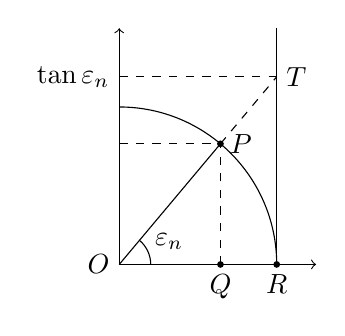
\begin{tikzpicture}[scale=2]
                \def\angle{50}

                \draw[->] (0,0) node[below, left] {\(O\)} -- (1.25,0);
                \draw[->] (0,0) -- (0,1.5);
                \draw (1,0) arc (0:90:1);
                \draw (0.2,0) arc (0:\angle:0.2);
                \node at (\angle*0.5:0.35) {\(\varepsilon_n\)};

                \draw[dashed] (0,{tan(\angle)}) -- (1,{tan(\angle)}) node[right] {\(T\)};
                \node[left] at (0, {tan(\angle)}) {\(\tan \varepsilon_n\)};

                \draw[-] (1,0) -- (1,1.5);
                
                \filldraw (\angle:1) circle (0.5pt);
                \draw[-] (0,0) -- (\angle:1) node[above, right] {\(P\)};
                \draw[dashed] (\angle:1) -- (\angle:{sqrt(1 + tan(\angle)*tan(\angle))});
                \draw[dashed] (0, {sin(\angle)}) -- ({cos(\angle)}, {sin(\angle)});

                \draw[dashed] ({cos(\angle)}, 0) -- (\angle:1);
                \filldraw ({cos(\angle)}, 0) node[below] {\(Q\)} circle (0.5pt);
                \filldraw (1, 0) node[below] {\(R\)} circle (0.5pt);
            \end{tikzpicture}
        \end{center}

        Per confronto di aree,
        l'area del triangolo \(OPQ\) è minore o uguale dell'area del settore circolare \(OPR\)
        che è minore o uguale del triangolo \(OTR\).
        
        Ricordiamo che l'area del settore circolare di angolo \(\alpha\) è data dalla proporzione
        \[
            \frac{\text{Area } S_\alpha}{\text{Area cerchio}} = \frac{\alpha}{2\pi}
        \]
        quindi
        \[
            \text{Area}_{OPR} = \frac{1}{2} \alpha
        \]
        Abbiamo allora che
        \[
            \frac{1}{2} \cos \varepsilon_n \sin \varepsilon_n
            \leq
            \frac{1}{2} \varepsilon_n
            \leq
            \frac{1}{2} \cdot 1 \cdot \tan \varepsilon_n
        \]
        che semplificando diventa
        \[
            \cos \varepsilon_n \leq \frac{\varepsilon_n}{\sin \varepsilon_n}
            \leq \frac{1}{\cos \varepsilon_n}
        \]
        Siccome \(\cos \varepsilon_n \to 1\) e \(\frac{1}{\cos \varepsilon_n} \to 1\),
        per il teorema dei carabinieri,
        \[
            \frac{\varepsilon_n}{\sin \varepsilon_n}
        \]
        Per la tangente abbiamo semplicemente
        \[
            \frac{\tan \varepsilon_n}{\varepsilon_n} = \left(\frac{\sin \varepsilon_n}{\varepsilon_n}\right)
            \left(\frac{1}{\cos \varepsilon_n}\right) \to 1
        \]
        E per il coseno abbiamo
        \begin{align*}
            \frac{1-\cos \varepsilon_n}{\varepsilon_n^2} &= \frac{
                (1 - \cos \varepsilon_n) ( 1 + \cos \varepsilon_n)
            }{
                \varepsilon_n^2 \cdot (1 + \cos \varepsilon_n)
            } \\
            &= \frac{1 - \cos^2 \varepsilon_n}{\varepsilon_n} \cdot \frac{1}{1 + \cos \varepsilon_n} \\
            &= {\left(\frac{\sin \varepsilon_n}{\varepsilon_n}\right)}^2 \left(\frac{1}{1 + \cos \varepsilon_n} \to \frac{1}{2}\right)
        \end{align*}
    \end{enumerate}
}

\sproposition{}{
    Calcolare il limite della successione
    \[
        a_n = (n+2)\sin\left(\frac{n+1}{n^2}\right)
    \]
    Notiamo che
    \[
        \varepsilon_n = \frac{n+1}{n^2} \to 0
    \]
    Scriviamo
    \begin{align*}
        a_n &= (n+2) \frac{\sin \varepsilon_n}{\varepsilon_n} \cdot \varepsilon_n \\
        &= \frac{\sin \varepsilon_n}{\varepsilon_n} \frac{(n+2)(n+1)}{n^2} \\
        &= \frac{\sin \varepsilon_n}{\varepsilon_n} \frac{n^2(1+\frac{2}{n})(1+\frac{1}{n})}{n^2}
        \to 1
    \end{align*}
}

\subsection{Proprietà asintotico}

\textbf{Nota:} non vale \(a_n \sim b_n \implies e^{a_n} \sim e^{b_n}\)
se \(a_n \to \infty\).
Per esempio, \(a_n = n + \sqrt{n} = n(1 + \frac{1}{\sqrt{n}}) \sim n = b_n\).
Quindi
\[
    \frac{e^{a_n}}{e^{b_n}} = e^{a_n-b_n} = e^{\sqrt{n}} \to +\infty
\]

\textbf{Nota:} non vale \(a_n \sim b_n \implies \log a_n \sim \log b_n\)
se \(a_n \to 1\).
Per esempio, \(a_n = 1 + \frac{1}{n}\) e \(b_n = 1 + \frac{1}{n^2}\).
Tuttavia,
\[
    \frac{\log a_n}{\log b_n} \to +\infty
\]

\textbf{Nota:} non vale \(a_n \sim b_n \land c_n \sim d_n \implies a_n \pm c_n \sim b_n \pm d_n\).
Per esempio, \(a_n = n + \sqrt{n} \sim n = b_n\).

\sproposition{Proprietà dell'o-piccolo}{
    \begin{itemize}
        \item Se \(a_n = o(b_n)\), allora \(a_n = \mathcal{O}(b_n)\);
        \item Se \(a_n = o(b_n)\) e \(c_n = \mathcal{O}(d_n)\),
        allora \(a_nc_n = o(b_nd_n)\). Infatti,
        \[
            \left|\frac{a_nc_n}{b_nd_n}\right| = \left|\frac{a_n}{b_n}\right| \left|\frac{c_n}{d_n}\right| 
        \]
        che tendono entrambi a zero;
        \item Se \(a_n = o(b_n)\) e \(c_n = o(b_n)\), allora \(a_n + c_n = o(b_n)\).
        Infatti,
        \[
            \frac{a_n + c_n}{b_n} = \frac{a_n}{b_n} + \frac{c_n}{b_n}
        \]
        che tendono entrambi a zero. Possiamo anche scrivere \(o(b_n) + o(b_n) = o(b_n)\);
    \end{itemize}
}

\subsection{Esercizi}

\sexercise{}{
    \[
        a_n = \frac{
            \log \left(\frac{n^2 + 1}{n}\right) + 1
        }{
            \sqrt{n^3 + 1} + \log n
        }
    \]
}

\sexercise{}{
    \[
        a_n = \frac{
            n^{1/2} + \cos(1/n) + \log n
        }{
            {(n + \sqrt{n})}^2 - \sqrt{n}
        }
    \]
}

\sexercise{}{
    \[
        a_n = \log \left(
            1 + \sin \left(\frac{\sqrt{n}}{n^2 + \log n}\right)
        \right)
        \left(\sqrt[3]{n^6 + 1} - n^2\right)
    \]
}

\sexercise{}{
    \[
        a_n = {\left(\cos \frac{1}{\sqrt{n}}\right)}^{\frac{n^3 - \log n}{\sqrt{n^4 + n}}}
    \]
}

\pagebreak 

\section{Serie numeriche}

\sexercise{}{
    Sia \(\{b_n\}\) una successione e sia \(\{b_{n\pm k_0}\}\) la successione traslata di
    \(\pm k\).
    Dimostrare che \(\lim b_n\) esiste se e solo se \(\lim b_{n \pm k_0}\) esiste e che i limiti sono uguali.
    % TODOURGENT
}

\sexample{}{
    Considera
    \[
        \sum_{n=1}^\infty \frac{1}{4n^2 - 1}
    \]
    Allora
    \[
        \frac{1}{4n^2 - 1} = \frac{1}{(2n+1)(2n-1)} = \frac{1/2}{2n-1} - \frac{1/2}{2n+1}
    \]
    Quindi
    \begin{align*}
        \frac{1}{2} \sum_{n=1}^\infty \left(\frac{1}{2n-1} - \frac{1}{2n+1}\right) \to
        \frac{1}{2}  
    \end{align*}
}

\sproof{Serie geometrica per Induzione}{
    %TODOURGENT
}

\sexample{}{
    Calcolare
    \[
        \sum_{n=0}^\infty {\left(\frac{1}{10}\right)}^n
    \]
    La serie ha ragione \(q = \frac{1}{10}\)
    e quindi
    \[
        \frac{1}{1 - \frac{1}{10}} = \frac{10}{9}
    \]
}

\sexercise{}{
    Calcolare
    \begin{align*}
        \sum_{n=1}^\infty \frac{3^n + 2\cdot 5^{n+1}}{7^{n+2}}
        &= \sum_{n=1}^\infty \frac{3^{n}}{7^{n+2}}
        + 2 \sum_{n=1}^\infty \frac{5^{n+1}}{7^{n+2}} \\
        &= \frac{1}{7^2} \sum_{n=1}^\infty \frac{3^{n}}{7^n}
        + \frac{2}{7} \sum_{n=1}^\infty \frac{5^{n+1}}{7^{n+1}} \\
        &= \frac{1}{7^2} \sum_{n=0}^\infty {\left(\frac{3}{7}\right)}^{n+1}
        +  \frac{2}{7} \sum_{n=0}^\infty {\left(\frac{3}{7}\right)}^{n+2} \\
        &= \cdots
    \end{align*}
}

\subsection{Aritmetica delle serie}

Le operazioni aritmetiche sulle serie sono giustificate a posteriori;
se alla fine vi è una forma di indecisione non erano legali.

\sproposition{}{
    Un numero decimale può essere espresso come
    \[
        x = N + \sum_{k=1}^\infty a_k \cdot 10^{-k}
    \]
}

\sexample{}{
    Mostriamo che se
    \(x = N, a_1 a_2 \cdots a_k \overline{9}\) dove \(a_j \in \{0,1,2,3,4,5,6,7,8,9\}\)
    e \(a_k < 9\),
    allora \(x = N a_1 a_2 \cdots (a_k + 1)\).
    Abbiamo quindi che
    \begin{align*}
        x &= N + \left( \sum_{j=1}^k a_j \cdot 10^{-j} \right)
        + \sum_{j=k+1}^\infty 9 \cdot 10^{-j} \\
        &= N + \left( \sum_{j=1}^{k-1} a_j \cdot 10^{-j} \right)
        + a_k \cdot 10^{-k} + 9\cdot 10^{-k-1}
        \sum_{h=0}^\infty 10^{-h} \\
        &= N + \left( \sum_{j=1}^{k-1} a_j \cdot 10^{-j} \right)
        + a_k \cdot 10^{-k} + 9 \cdot 10^{-k-1} \cdot \frac{10}{9} \\
        &= N + \left( \sum_{j=1}^{k-1} a_j \cdot 10^{-j}\right) + 10^{-k}(a_k + 1)
    \end{align*}
    Ciò può essere esteso ad ogni base.
}

\scorollary{}{
    Se \(a_n = o(b_n)\) cioè
    \[
        \frac{a_n}{b_n} \to 0
    \]
    per definizione di limite, fissato \(\varepsilon = 1\),
    esiste \(n_0\) tale che \(0 < \frac{a_n}{b_n} < 1 \implies 0 \leq a_n \leq b_n\)
    e quindi si applica il confronto.
}

\sexercise{}{
    Stabilire il carattere della serie
    \[
        \sum_{n=1}^\infty \frac{n^2 + {(1 + 1/n)}^n + \sin n}{{(n+\sqrt{n})}^3 + \log \left(\frac{n}{n+1}\right)}
    \]
    Notiamo che \(\forall n \geq 1, a_n \geq 0\).
    Notiamo allora che
    \[
        a_n = \frac{n^2 \left(1 + \frac{1}{n^2}{\left(1 + \frac{1}{n}\right)}^n + \frac{\sin n}{n}\right)}
        {n^3 \left\{{\left(1 + \frac{1}{\sqrt{n}}\right)}^3 + \frac{1}{n^3}\log\left(\frac{n}{n+1}\right)\right\}}
        \sim \frac{1}{n}
    \]
    Siccome la serie armonica è una serie-p con \(p=1\), allora la serie diverge.
}

\sexample{Teorema di condensazione}{
    È possibile applicare il teorema di condensazione alla serie armonica
    e ottenere che
    \[
        \sum_{k=0}^\infty {\left(\frac{1}{2^{p-1}}\right)}^k
    \]
    che è una serie geometrica di ragione
    \(\frac{1}{2^{p-1}}\) che converge se e solo se \(p>1\).
}

\stheorem{Rapporto di radici}{
    Sia \(\sum a_n\) una serie a termini \(\geq 0\) e supponiamo che
    una delle due condizioni sia soddisfatta:
    \begin{enumerate}
        \item \(\exists\, \underset{n}{\lim}\, \sqrt[n]{a_n} = L \in [0; +\infty]\);
        \item \(a_n > 0\) definitivamente e
            \(\exists\, \underset{n}{\lim}\, \frac{a_{n+1}}{a_n} = h \in [0; +\infty]\);
    \end{enumerate}
    Allora se \(L < 1\) la serie converge, mentre se \(L > 1\) allora
    \(a_n \to \infty\).
}

Se \(L=1\) il test è \textbf{inclonclusivo}.

La condizione della radice è più potente in quanto implica anche l'altra.

Infatti, con la p-serie armonica il limite tende a \(1\), il che coincide
con il fatto che la serie converge se \(p > 1\) e diverge altrimenti.

\scorollary{}{
    Sia \(\{a_n\}\) una successione con \(a_n \geq 0\).
    Se
    \[
        \exists\, \underset{n}{\lim}\, \sqrt[n]{a_n} = L
    \]
    oppure se il limite esiste e \(a_n \neq 0\) definitivamente,
    allora se \(L<1\), la serie converge e \(a_n \to 0\)
    e se \(L>1\) allora \(a_n \to +\infty\).
}

\sproof{}{
    Consideriamo il primo caso cosicché
    \[
        \exists\, \underset{n}{\lim}\, \sqrt[n]{a_n} = L
    \]
    Per definizione di limite, \(\forall \varepsilon > 0\) fissato
    \(\exists\, N\) tale che
    \[
        L-\varepsilon < \sqrt[n]{a_n} < L + \varepsilon
    \]
    Se \(L < 1\), esiste \(\varepsilon > 0\) tale che
    \(L+\varepsilon < 1\) (basta scegliere \(\varepsilon = (1-L)/2\)).
    Dalla disequazione \(\sqrt[n]{a_n} < L + \varepsilon\) deduciamo che
    \[
        \forall n \geq N, 0 \leq a_n < {(L+\varepsilon)}^n
    \]
    e poiché \(L+\varepsilon<1\) la serie converge per confronto
    con la serie geometrica
    \[
        \sum^\infty {(L+\varepsilon)}^n
    \]
    Se \(L > 1\) allora esiste \(\varepsilon > 0\)
    tale che \(L - \varepsilon > 1\), come per esempio
    \(\varepsilon = \frac{L-1}{2}\), quindi per \(n\geq N\) abbiamo
    \[
        \sqrt[n]{a_n} > (L - \varepsilon) > 1
    \]
    elevando alla \(n\) otteniamo \(a_n > {(L-\varepsilon)}^n \to +\infty\)
    e per confronto \(a_n \to +\infty\).
    In particolare, \(a_n\) non tende a zero e la serie diverge per il criterio
    del termine ennesimo.

    Per il secondo caso, \(\exists\, \underset{n}{\lim}\, \frac{a_{n+1}{a_n}} = L\)
    come nel caso precedente. Quindi \(\forall \varepsilon > 0\)
    esiste \(N\) tale che 
    \[
        L - \varepsilon < \frac{a_{n+1}}{a_n} < L + \varepsilon
    \]
    Sappiamo per esempio che \(L > 1\) cosicché come nel caso precedente
    possiamo scegliere \(\varepsilon\) tale che
    \(L - \varepsilon > 1\) e abbiamo che \(\forall n \geq N\)
    \[
        \frac{a_{n+1}}{a_n} > L - \varepsilon > 1 > 0
    \]
    \(\forall n \geq N\) moltiplicando i termini membro a membro
    \[
        \frac{a_{N+1}}{a_N} \cdot
        \frac{a_{N+2}}{a_{N+1}} \cdot
        \frac{a_{N+3}}{a_{N+2}} \cdots
        \frac{a_{n}}{a_{n-1}} \cdot
        \frac{a_{n+1}}{a_{N}}
        = \frac{a_{n+1}}{a_{N}} \geq {(L-\varepsilon)}^{n-N+1}
    \]
    Ciascuno di questi è più grande di \(L - \varepsilon\).
    Quindi,
    \[
        a_{n+1} \geq {(L-\varepsilon)}^{-N+1}
        \cdot
        {(L-\varepsilon)}^n \cdot a_N \to +\infty
    \]
    e per confronto \(a_n \to +\infty\).
}

\sexample{}{
    Consider
    \[
        \sum_{n=1}^\infty \frac{A^n}{n!}
    \]
    con \(A > 0\).
    Quando ci sono i fattoriali usiamo il criterio dei rapporti.
    Abbiamo che
    \[
        \forall n, a_n = \frac{A^n}{n!} > 0
    \]
    per il criterio del rapporto
    \begin{align*}
        \frac{a_{n+1}}{a_n} = \frac{A^n}{(n+1)!}
        \cdot \frac{n!}{A^n} = \frac{A}{n+1} \to 0
    \end{align*}
    Quindi la serie converge, e converge a \(e^A - 1\).
}

\sexample{}{
    Consider
    \[
        \sum_{n=1}^\infty \frac{e^{n^2} + {(\log n)}^n + {\left(1 + \frac{1}{n}\right)}^n}{n^n + e^{3n\log n} + {\left(n+\frac{1}{n}\right)}^{17}}
    \]
    che è ovviamente positivo.
    Usiamo il criterio asintotito.
    A numeratore l'ultimo termine è finito e tende ad \(e\).
    Dobbiamo verificare quale degli altri due termini è dominante.
    Scriviamo allora \({(\log n)}^n = e^{n\log\log n}\).
    Allora chiaramente \(e^{n^2}\) domincia sull'altro termine.
    Analogamente, a denominatore abbiamo \(n^n = e^{n\log n}\)
    come termine dominante.
    \[
        a_n =  \frac{
            e^{n^2} \left\{
            1 + e^{n\log \log(n) - n^2}
            + {\left(1 + \frac{1}{n}\right)}^{n} \cdot e^{-n^2}
        \right\}
        }{
            e^{3n\log n} \left\{
                1 + e^{-2n\log n} + {\left(1 + \frac{1}{n}\right)}^{17}
                \cdot e^{-3n\log n}
            \right\}
        } \sim \frac{e^{n^2}}{e^{3n\log n}}
    \]
    Allora
    \[
        e^{n\log \log n - n^2} = e^{-n^2 \left\{1 - \frac{\log\log n}{n^2}\right\}}
        \to \infty
    \]
    quindi la serie diverge.
    Oppure, con il criterio della radice
    \[
        {\left(e^{n^2 - 3n \log n}\right)}^{\frac{1}{n}}
        = e^{n\left(1 - \frac{3\log n}{n}\right)} \to \infty > 1
    \]
}

\sexample{}{
    Studiare il carattere di
    \[
        \sum^\infty \frac{
            n^{n\log n}
        }{
            (2n)!
        }
    \]
    che ha termini positivi. Ci sono dei fattoriali quindi conviene utilizzare il criterio
    del rapporto.
    Notiamo che \((2n+2)! = (2n+2)(2n+2)(2n)!\)
    e \((n+1)\log(n+1) = n\log(n+1) + \log(n+1) = n[\log n + \log(1 + 1/n)] + \log(n+1)\).
    Il rapporto è dato da\begin{align*}
        \frac{a_{n+1}}{a_n} &= \frac{
            {(n+1)}^{(n+1)\log(n+1)}
        }{
            (2n+2)!
        }
        \cdot
        \frac{
            (2n)!
        }{
            n^{n\log n}
        } \\
        &= \frac{
            {(n+1)}^{n\log n} \cdot {(n+1)}^{n\log(1 + 1/n) + \log(n+1)}
        }{
            n^{n\log n}
        }
    \end{align*}
    Con
    \[
        {\left(1 + \frac{1}{n}\right)}^{n\log n}
        \cdot {(n+1)}^{n\log(1 + 1/n)}
        \cdot {(n+1)}^{\log (n+1)}
    \]
    troviamo
    \[
        \frac{1}{((2n+2)(2n+1))} \cdot {\left[
            {\left(1 + \frac{1}{n}\right)}^n
        \right]}^{\log n}
        \cdot {(n+1)}^{n\log (1 + 1/n)}{(n+1)}^{\log(n+1)}
    \]
    Dal primo e ultimo termine possiamo notare che la serie va ad infinito.
}

\sexample{}{
    Considera
    \[
        \sum_{n=1}^\infty
        \frac{
            2^{\sqrt{n}}
        }{
            n^{\log n}
        }
    \]
    Il criterio della radice non funziona. Infatti,
    \begin{align*}
        \sqrt[n]{a_n}
        = \frac{
            2^{1 / \sqrt{n}}
        }{
            n^{\frac{\log n}{n}}
        }
    \end{align*}
    Il numeratore tende a \(1\),
    mentre scriviamo il denominatore come
    \begin{align*}
        n^{\frac{\log n}{n}} &=
        e^{\frac{1}{n}\log \left(n^{\log n}\right)} \\
        &= e^{\frac{1}{2}{\left(\log n\right)}^2} \to 1
    \end{align*}
    Allora il limite è \(L=1\), quindi il criterio è inconclusivo.
    Allora
    \begin{align*}
        a_n &= \frac{
            a^{\sqrt{n}\log 2}
        }{
            e^{{(\log n)}^2}
        } \\
        &= e^{\sqrt{n} \log 2 - {\left(\log n\right)}^2} \\
        &= e^{\sqrt{n} \left\{\log 2 - \frac{{\log n}^2}{\sqrt{n}}\right\}}
    \end{align*}
    L'esponente tende a infinito quindi la serie diverge per il criterio
    del termine n-esimo.
}

\sexample{}{
    \[
        \sum_{n=1}^\infty
        \frac{
            n^{\log n}
        }{
            2^{\sqrt{n}}
        }
    \]
    che ha i termini della serie precedente ma invertiti.
    Dobbiamo usare il confronto per mostrare che la serie converge.
    Confrontiamo la serie con una p-serie, per esempio \(\sum\frac{1}{n^2}\).
    Il rapporto è dato da
    \begin{align*}
        \frac{a_n}{\frac{1}{n^2}}
        &= n^2 a_n  \\
        &= e^{2\log n - \sqrt{n}\left\{\log 2 - \frac{{(\log n)}^2}{\sqrt{n}}\right\}}
    \end{align*}
    e abbiamo che
    \begin{align*}
        2\log n - \sqrt{n}\log 2 + {(\log n)}^2
        = -\sqrt{n} \left\{
            \log 2 - \frac{2\log n}{\sqrt{n}}
            - \frac{{(\log n)}^2}{\sqrt{n}} \to -\infty
        \right\}
    \end{align*}
    e quindi il rapporto tende a \(0\). Quindi,
    il rapporto è minore di 1 definitivamente
    e la serie converge per confronto.
}

\subsection{Formula di Stirling}

\sexample{}{
    Studia il carattere di
    \[
        \sum_{n=1}^\infty \frac{n^n}{(2n)!}
    \]
    Il limite è dato da
    \begin{align*}
        \frac{a_{n+1}}{a_n} = \frac{
            {(n+1)}^{n+1}
        }{
            (2n+2)!
        }
        \cdot
        \frac{
            (2n)!
        }{
            n^n
        }
        &=
        {\left(\frac{n+1}{n}\right)}^n
        \frac{
            (n+1)(2n)!
        }{
            (2n+2)(2n+1)(2n)!
        } \\
        &=
        {\left(\frac{n+1}{n}\right)}^n
        \frac{n+1}{(2n+2)(2n)!}
        \sim e \cdot  \frac{
            n+1
        }{
            (2n+2)(2n+1)
        } \\
        &= \frac{e^{n(1+1/n)}}{{(2n)}^2 {\left(1 + \frac{1}{n}\right)}{\left(1 + \frac{1}{2n}\right)}}
        \to 0
    \end{align*}
    Quindi la serie converge.

    Con radici abbiamo
    \begin{align*}
        {\left[\frac{n^n}{(2n)!}\right]}^{1/n}
        &= \frac{n}{
            {\left[
                {(2n)}^{2n}
                \cdot 2^{-2n} \cdot \sqrt{4\pi n}(1 + o(1))
            \right]}^{1/n}
        } \\
        &= \frac{n}{
            {(2n)}^2 \cdot e^{-2} {(4\pi)}^{\frac{1}{2n}}
            \cdot n^{\frac{1}{2n}}{(1 + o(1))}^{\frac{1}{n}}
        } \to 0
    \end{align*}
    E quindi converge
}

\sexample{}{
    Studia il carattere di
    \[
        \sum_{n=1}^\infty \frac{e^{n^2} + n^n}{(n^2)! + {\left(1 + \frac{1}{n}\right)}^{n^2}}
    \]
    A numeratore abbiamo
    \begin{align*}
        e^{n^2} + n^n = e^{n^2} + e^{n \log n} = e^{n^2}
        \left\{1 + e^{n\log n - n^2}\right\}
        \sim e^{n^2}
    \end{align*}
    A denominatore abbiamo
    \begin{align*}
        (n^2)! + {\left(1 + \frac{1}{n}\right)}^{n^2}
        &= {(n^2)}^{n^2} \cdot e^{-n^2}
        \cdot \sqrt{2\pi n^2}(1 + o(1))
        + e^{n^2 \log \left(1 + \frac{1}{n}\right)} \\
        &= e^{2n^2 \left\{
            \log n - \frac{1}{2} + \frac{1}{2n^2} \log \sqrt{2\pi n^2}
        \right\}}(1 + o(1)) + e^{n^2 \log\left(1 + \frac{1}{n}\right)}
        \\
        &= e^{2n^2 \left\{
            \log n - \frac{1}{2} + \frac{1}{2n^2} \log\sqrt{2\pi n^2}
        \right\}}
        \left\{1 + o(1) + e^{n^2\log\left(1 + \frac{1}{n}\right) - 2n^2 \left\{\cdots\right\}}\right\} \\
        &\sim e^{2n^2 \left\{
            \log n - \frac{1}{n} + \frac{1}{2n^2}
            \log\sqrt{2\pi n^2}
        \right\}}
        = {(n^2)}^{n^2} e^{-n^2} \sqrt{2\pi n^2}
    \end{align*}
    Ora possiamo usare il criterio della radice
    \begin{align*}
        a_n \sim \frac{
            e^{n^2}
        }{
            {(n^2)}^{n^2}
            e^{-n^2}
            \sqrt{2\pi n^2}
        }
        = b_n
    \end{align*}
    Abbiamo che \(\sum a_n\) ha lo stesso carattere di \(\sum b_n\)
    e
    \begin{align*}
        \sqrt[n]{b_n} &= \frac{
            e^n
        }{
            {(n^2)}^n e^{-n}
            {(2n)}^{\frac{1}{2n}} n^{1/n}
        } \\
        &= \frac{
            e^{2n}
        }{
            n^{2n} {(2n)}^{1/n} n^{1/n}
        } \to
        0
    \end{align*}
    e quindi la serie converge.
}

\pagebreak

\subsection{Serie a termini di segno qualunque}

Con serie di segno qualunque non è possibile applicare il criterio asintotico.

Sia \(\{a_n\}\) una successione reale o complessa (o in uno spazio metrico)
e supponiamo che esista finito il limite \(\underset{n}{\lim}\, a_n = L \in \mathbb{F}\).
Per definizione di limite, \[\forall \varepsilon > 0, \exists\, N \,|\, \forall n \geq N,
|a_n - L| < \varepsilon\]
Quindi, se \(n,m > N\), allora
\[
    |a_n - a_m| = |(a_n - L) + (L - a_m)|
    \trianglelefteqslant
    |a_n - L| + |L - a_m|
    < 2 \varepsilon
\]

\sdefinition{Successione di Cauchy}{
    Sia \(\{a_n\}\) una successione reale o complessa.
    Si dice che \(\{a_n\}\) soddisfa la condizione (C) di Cauchy, o più brevemente
    che è una successione di Cauchy,
    se
    \[
        \forall \varepsilon > 0, \exists\, n \,|\,
        \forall n,m \geq M,
        |a_n - a_m| < \varepsilon
    \]
    Per quanto visto sopra, se \(a_n \to L\) finito, allora \(\{a_n\}\)
    è di Cauchy.
}

\stheorem{}{
    Sia \(\{a_n\}\) una successione reale o complessa.
    Sono equivalenti:
    \begin{enumerate}
        \item \(\exists\) finito
        \[
            \underset{n}{\lim}\, a_n = L
        \]
        \item \(\{a_n\}\) è una successione di Cauchy.
    \end{enumerate}
}

Abbiamo visto che (1) implica (2). Il converso, vale in \(\mathbb{R}\)
ma non in \(\mathbb{Q}\).

\sproposition{}{
    Sia
    \[
        \sum^\infty a_n
    \]
    una serie reali o complessa e sia \(\{S_N\}\)
    la successione delle sue somme parziali.
    Per definizione, \(\sum a_n\) converge a \(S\) se esiste
    finito \(\underset{n}{\lim}\, S_n \in \mathbb{R}\).
}

\scorollary{}{
    Condizione necessaria e sufficiente perché una serie \(\sum a_n\) converga
    e che la successione delle somme parziali soddisfi le condizioni di Cauchy, scritte
    in 3 modi equivalenti:
    \begin{enumerate}
        \item \[ \forall \varepsilon > 0, \exists\, N \,|\, \forall n,m \geq N, |S_N - S_M| < \varepsilon\]
        equivalentmeente notando che se \(n>m\), \[S_n - S_m = \sum_{k=1}^n a_k - \sum_{k=1}^m a_k = \sum_{m+1}^{n} a_k\]
        \item \[
            \forall \varepsilon > 0, \exists\, N \,|\, \forall n,m \geq N
            \quad n>m \quad \left|\sum_{k=m+1}^n a_k\right| < \varepsilon
        \]
        ovvero
        \[
            \forall \varepsilon > 0, \exists\, N \,|\, \forall n,m \geq N
            \quad n\geq m \quad \left|\sum_{k=m+1}^n a_k\right| < \varepsilon
        \]
        \item \textbf{condizione più usata:}
        \[
            \forall \varepsilon > 0, \exists\, N \,|\,
            \forall m,n \geq N \land \forall p \geq 0, \left|\sum_{k=m}^{m+p} a_k\right|
            < \varepsilon
        \]
    \end{enumerate}
}

La serie
\[
    \sum_{n=1}^\infty \frac{{(-1)}^n}{n^p}
\]
con \(0 < p \leq 1\) converge ma non assolutamente.
La serie converge per \(p > 0\).

\slemma{disuguaglianza triangolare generalizzata}{
    Sia \(\{b_k\}\) una successione,
    allora
    \[
        \left|\sum_{k=1}^n b_k\right|
        \leq
        \sum_{k=1}^n |b_k|
    \]
}

\sproof{}{
    Per induzione
    \begin{itemize}
        \item il caso base è banale;
        \item \begin{align*}
            \left|
                \sum_{k=1}^{n + 1} b_k
            \right|
            &= \left|
                \left(
                    \sum_{k=1}^{n} b_k
                \right)
                + b_{n+1}
            \right|
            \trianglelefteqslant \left|
                \sum_{k=1}^{n} b_k
            \right|
            + |b_{n+1}| \\
            &= \sum_{k=1}^{n} |b_k|
            + |b_{n+1}| = \sum_{k=1}^{n+1} |b_k|
        \end{align*}
    \end{itemize}
}

\sproof{Teorema fondamentale}{
    Sapendo che
    \[
        \sum_{k=1}^\infty |a_k| < +\infty
    \]
    la tesi è che
    \[
        \sum_{k=1}^\infty a_k
    \]
    converga equivalentemente soddisfa le condizionid i Cauchy.
    \[
        \forall \varepsilon > 0, \exists\, N \,|\,
        \forall n \geq m \geq N, \left|\sum_{k=m}^n a_k\right| \leq \varepsilon
    \]
    Per ipotesi \(\sum |a_k|\) converge quindi soddisfa la condizione di Cauchy
    e dato \(\varepsilon > 0\), esiste \(N\) tale che \(\forall n \geq m \geq N\)
    \[
    \left|
        \sum_{k=m}^n |a_k|
    \right|
    = \sum_{k=m}^n |a_k| \varepsilon
    \]
    Ma per il lemma \(\forall n \geq m \geq N\),
    \[
        \left|
        \sum_{k=m}^n a_k
        \right|
        \leq \sum_{k=m}^n |a_k| < \varepsilon
    \]
}

Quando abbiamo una serie che non ha termini solo positivi, la prima cosa da fare
è mettere il modulo e controllare la convergenza assoluta.

\sexample{}{
    Considera
    \[
        \sum \frac{\sin n}{n^2}
    \]
    che non ha termini solo positivi. Allora proviamo a studiare la convergenza assoluta.
    \[
        \sum \frac{|\sin n|}{n^2}
    \]
    Poiché \(\frac{|\sin n|}{n^2} \leq \frac{1}{n^2}\)
    e \(\sum \frac{1}{n^2 \leq +\infty}\)
    converge (p-serie), allora la serie dei moduli converge assolutamente e quindi converge.
}

Vale lo stesso procedimento per
\[
    \sum \frac{\sin n}{n^p}
\]
con \(p > 1\).
Se \(p \leq 1\), allora diverge. Ciò segue dal fatto che, per esempio,
\(|\sin x| > \frac{1}{2}\) se \(\frac{\pi}{6} + k\pi \leq x \leq \frac{5}{6}\pi + k\pi\)
con \(k\in\mathbb{Z}\). Notiamo che l'intervallo
\[
    I_k = \left[\frac{\pi}{6} + k\pi; \frac{5}{6}\pi + k\pi\right]
\]
ha lunghezza \(\frac{2\pi}{3} > 1\), quindi conviene un interno \(n\),
in realtà \(2\) interi in quando la lunghezza è maggiore di \(2\).
Allora la serie \[
    \sum \frac{|\sin n|}{n}
    \geq 
    \sum_{k\in\mathbb{N}} \frac{|\sin n_k|}{n_k}
\]
dove \(n_k\) è un intero in ognuno di \(I_k\).
Ciò è maggiore o uguale di
\[
    \sum \frac{\frac{1}{2}}{\frac{5}{6} \pi + k\pi}
\]
in quanto il valore a denominatore è al minomo \(\frac{5}{6} \pi + k\pi\).
Allora troviamo un multiplo della serie armonica, che diverge.

\sexample{}{
    Considera
    \[
        \sum \frac{
            -n + {(\sin n)}n^2 - \log n
        }{
            {(1+n)}^{10/3} - \cos n
        }
    \]
    allora guardiamo il modulo:
    \[
        |a_n| = \frac{
            |-n + (\sin n)n^2 - \log n|
        }{
            |{(1+n)}^{10/3} - \cos n|
        }
    \]
    Maggioriamo rendendo più piccolo il denominatore e più grande il numeratore.
    \[
        |a_n| \leq \frac{
            n + n^2|\sin n| + |\log n|
        }{
            {(1+n)}^{10/3} -1
        }
    \]
    Notiamo che \({(1+n)}^{10/3} - 1 \geq \frac{1}{2}{(1+n)}^{10/3} > \frac{1}{2}n^{10/3}\)
    perché \(n=1\) dà il valore massimo. Quindi
    \[
        |a_n| \leq \frac{
           n
        }{
            \frac{1}{2}n^{10/3}         
        }
        + \frac{n^2}{\frac{1}{2}n^{10/3}}
        + \frac{\log n}{\frac{1}{2}n^{10/3}}
    \]
    Quindi
    \[
        \sum_{n=1}^\infty |a_n| \leq
        2 \sum n^{-\frac{7}{8}}
        +
        2 \sum n^{-\frac{4}{3}}
        + 2 \sum_{n=2} \frac{1}{n^{10/3} {(\log n)}^{-1}}
    \]
    Tutti i termini convergono e quindi la serie converge.
}

Perché il teorema valga basta che \(a_n \geq 0\) e \(a_n \geq a_{n+1}\)
valgano definitivamente.
In tal caso la stima dell'errore vale solo per \(n\) sufficientemente grande.

\sexample{}{
    Si può applicare il teorema a
    \[
        \sum_{n=1}^\infty \frac{{(-1)}^n}{n^p}
    \]
    e notare che la serie converge semplicemente ma non assolutamente per ogni \(0 < p \leq 1\).
}

\pagebreak

\sexample{}{
    Considera
    \[
        \sum_{n=1}^\infty {(-1)}^n a_n
    \]
    con
    \[
        a_n = \begin{cases}
            \frac{1}{n^2} & n \text{ pari} \\
            \frac{1}{n^4} & n \text{ dispari}
        \end{cases}
    \]
    Poiché \(\forall n \geq 1\), \(a_n \leq \frac{1}{n^2}\) e quindi \(p = 2 > 1\) e quindi la serie converge assolutamente,
    e quindi converge. Tuttavia, è chiaro che \(\forall n, a_{2n+1} < a_{2n+2}\).
}

\textbf{Nota:}
\(a_n \sim b_n\) e \(b_n\) monotona crescente non implica necessariamente che \(a_n\) sia monotona
decrescente.

Infatti,
\sexample{}{
    Consideriamo
    \[
        a_n = \frac{1}{\sqrt{n}} + {(-1)}^n \frac{1}{n}
    \]
    e \(b_n = \frac{1}{\sqrt{n}}\).
    È chiaro che \(b_n\) è strettamente monotona decrescente.
    Inoltre, \[
        a_n = \frac{1}{\sqrt{n}} \left\{
            1 + {(-1)}^n \frac{1}{\sqrt{n}}
        \right\} \sim
        \frac{1}{\sqrt{n}} = b_n
    \]
    Verifichiamo allora che
    \[
        a_{2k} > a_{2k-1}
    \]
    Infatti, \(a_n\) non può essere definitivamente monotona decrescente in quanto
    se \(a_n\) fosse definitivamente monotona decrescente, allora la serie
    \[
        \sum_{n=1}^\infty {(-1)}^n a_n
    \]
    per il teorema di Leibniz sarebbe convergente.
    Tuttavia,
    \begin{align*}
        \sum_{n=1}^\infty {(-1)}^n \left\{
            \frac{1}{\sqrt{n}} + {(-1)}^n \frac{1}{n}
        \right\}
        &=  \sum_{n=1}^\infty \left\{
            {(-1)}^n \frac{1}{\sqrt{n}} + \frac{1}{n}
        \right\} \\
        &= \sum_{n=1}^\infty \left( {(-1)}^n \frac{1}{\sqrt{n}} \right)
        + \sum_{n=1}^\infty \left( \frac{1}{\sqrt{n}} \right)
    \end{align*}
    dove il secondo addendo chiaramente diverge.
    Allora, la serie di partenza diverge, nonostante il primo addendo converga.
}

\pagebreak

\sexample{Stima errore teorema Leibniz}{
    Calcolare la somma della serie
    \[
        \sum_{n=0}^\infty \frac{{(-1)}^n}{n!} = e^{-1}
    \]
    con un errore minore di \(10^{-3}\).
    Abbiamo allora
    \[
        a_n = \frac{1}{n!}
    \]
    e \[
        \frac{a_{n+1}}{a_n} = \frac{1}{n+1} \to 0
    \]
    La serie converge assolutamente per il criterio della radice e per il criterio del rapporto.
    La serie è a termini alterni, \(a_n \to 0\) e \(a_{n+1} < a_n\), quindi vale la condizione per il teorema di Leibniz.
    Per l'errore abbiamo
    \[
        \forall N, |E_N| = |S - S_n| < \frac{1}{(N+1)!}
    \]
    Se noi imponiamo che \(\frac{1}{(N+1)!} < 10^{-3}\) certamente \(|E_N| < 10^{-3}\).
    Dobbiamo usare almeno \(N=6\) per ottenere \((N+1)!=5040 > 1000\).
    Allora,
    \[
        \sum_{n=0}^\infty \frac{{(-1)}^n}{n!} = 1 - \frac{1}{1} + \frac{1}{2!} - \frac{1}{3!}
        \cdots + \frac{1}{6!} = S_6
    \]
    che ha un errore minore o uguale di \(\frac{1}{6!}\).
}

\sexample{}{
    Studiare
    \[
        \sum_{n=1}^\infty {(-1)}^n \frac{\sqrt{n}}{n+1}
    \]
    la serie ha termini alterni con \(a_n = \frac{\sqrt{n}}{n+1}\).
    Controlliamo la convergenza assoluta:
    \begin{align*}
        a_n = \frac{1}{\sqrt{n}} \frac{1}{(1+1/n)} \sim \frac{1}{n^{1/2}}
    \end{align*}
    e
    \[
        \sum \frac{1}{n^{1/2}} = +\infty
    \]
    in quanto \(p = \frac{1}{2} \leq 1\) e quindi non converge assolutamente.
    Vogliamo ora usare il teorema di Leibniz.
    Le condizioni sono soddisfatte in quanto \(a_n \geq 0\) e \(a_n \sim \frac{1}{\sqrt{n}}\).
    Verifichiamo esplicitamente
    \begin{align*}
        a_n - a_{n+1} &= \frac{\sqrt{n}}{n+1} - \frac{\sqrt{n-1}}{n+2} \\
        &= \frac{\sqrt{n}(n+1)-{(n+1)}^{3/2}}{(n+1)(n+2)}
    \end{align*}
    Studiamo allora quando il numeratore è maggiore di zero.
    \begin{align*}
        \sqrt{n}(n+2) \geq {(n+1)}^{3/2}
    \end{align*}
    Siccome i termini sono tutti positivi, possiamo fare il quadrato
    \begin{align*}
        n{(n+2)}^2 \geq {(n+1)}^3 &= n^3 + 4n^2 + 4n \\
        & \geq n^3 + 3n^2 + 3n + 1
    \end{align*}
    che è sempre vero.
    Alternativamente, potremmo fare il limite con \(n \to \infty\) del numeratore
    \begin{align*}
        \sqrt{n}(n+2) - {(n+1)}^{3/2} &= n^{3/2} \left\{
            1 - \frac{2}{n} - {\left(1 + \frac{1}{n}\right)}^{3/2}
        \right\}
    \end{align*}
    Abbiamo che
    \begin{align*}
        \frac{2}{n} + 1- \left(1 + \frac{1}{n}\right)^{3/2} &= \frac{2}{n} - \left\{
            {\left(1+\frac{1}{n}\right)}^{3/2} - 1
        \right\}
    \end{align*}
    e
    \begin{align*}
        {\left(1+\frac{1}{n}\right)}^{3/2} - 1 \sim {(1+\varepsilon_n)}^{\alpha} - 1
        \sim \alpha \varepsilon_n
    \end{align*}
    e quindi
    \begin{align*}
        \frac{2}{n} - \left\{
            {\left(1+\frac{1}{n}\right)}^{3/2} - 1
        \right\}
        &= \frac{2}{n} - \frac{3}{2}\frac{1}{n} (1 + o(1)) \\
        &= \frac{1}{2n} - \frac{3}{2}\frac{1}{n}o(1) \\
        &= \frac{1}{2n} + \frac{1}{n}o(1) \\
        &= \frac{1}{n} \left\{\frac{1}{2} + o(1)\right\} \\
        &\sim \frac{1}{2n}
    \end{align*}
    Adesso, per permanenza del segno, il fatto che il numeratore tenda ad infinito, implica che sia maggiore di zero
    definitivamente.
    Allora, possiamo utilizzare il teorema di Leibniz.
    Alternativamente, se non risuciamo a mostrare che i termini siano decrescente, abbiamo
    \[a_n = \frac{\sqrt{n}}{n+1} \sim \frac{1}{\sqrt{n}} = b_n\]
    e \(b_n\) è decrescente. Allora, scriviamo \[
        a_n = \frac{1}{\sqrt{n}} + \left(\sqrt{n}{n+1} - \frac{1}{\sqrt{n}}\right)
    \]
    Cosifacendo, abbiamo che
    \begin{align*}
        \sum_{n=1}^infty {(-1)}^n a_n &= \sum_{n=1}^\infty \left\{ {(-1)}^n \frac{1}{\sqrt{n}} + {(-1)}^n \left(
            \frac{\sqrt{\sqrt{n}}}{n+1} - \frac{1}{\sqrt{n}}
        \right)\right\} \\
        &= \sum_{n=1}^\infty {(-1)}^n \frac{1}{\sqrt{n}} + \sum_{n=1}^\infty {(-1)}^n
        \left(\frac{\sqrt{n}}{n+1} - \frac{1}{\sqrt{n}}\right)
    \end{align*}
    Se non ci sono forme di intedeterminazione nel membro di destra,
    \begin{align*}
        \sum^\infty {(-1)}^n \frac{1}{\sqrt{n}}
    \end{align*}
    converge semplicemente ma non assolutamente per il teorema di Leibniz.
    La seconda serie
    \begin{align*}
        \sum {(-1)}^n \left(
            \frac{\sqrt{n}}{n+1} - \frac{1}{\sqrt{n}}
        \right)
    \end{align*}
    ha modulo
    \begin{align*}
        \left| \frac{\sqrt{n}}{n+1} - \frac{1}{\sqrt{n}} \right| &= \frac{1}{\sqrt{n}} - \frac{\sqrt{n}}{n+1} \\
            &= \frac{(n+1) - \sqrt{n}\sqrt{n}}{\sqrt{n}(n+1)} \\
            &= \frac{1}{\sqrt{n}(n+1)} \\
            &= \frac{1}{n^{3/2}(1 + 1/n)} \sim \frac{1}{n^{3/2}}
    \end{align*}
    Concludiamo quindi che
    \[
        \sum {(-1)}^n a_n
    \]
    converge come somma di
    \[
        \sum {(-1)}^n \frac{1}{\sqrt{n}}
    \]
    che converge semplicemente ma non assolutamente e
    \[
        \sum {(-1)}^n \left( \frac{\sqrt{n}}{n+1} - \frac{1}{\sqrt{n}} \right)
    \]
    che converge assolutamente e la convergenza non può essere assoluta perché
    se \(\sum a_n\) e \(\sum b_n\) convergano assolutamente allora \(\sum (a_n + b_n)\)
    converge assolutamente. Infatti,
    \[
        \sum |a_n - b_n| \leq \sum (|a_n| + |b_n|)
        = \sum |a_n| + \sum |b_n| < +\infty
    \]
}

\subsection{Serie con parametri}

\sexample{}{
    Considera
    \[
        \sum_{n=1}^\infty \frac{\log n}{n+1}{\left(x^2-x-2\right)}^2
    \]
    Controlliamo la positività
    \begin{align*}
        x^2 - x - 2 \geq 0
    \end{align*}
    per \(x \leq - 1 \lor x \geq 2\), altrimenti i termini sono alterni.
    Studiamo la convergenza assoluta usando il criterio di radice/rapporto
    \begin{align*}
        {\left|\frac{\log n}{n+1}(x^2 - x - 2)\right|}^{1/n}
        &= \frac{{\left(\log n\right)}^{1/n}}{{\left[n(1+1/n)\right]}^{1/n}}
    \end{align*}
    Scriviamo che \({\left(\log n\right)}^{1/n} = e^{\frac{1}{n}\log\log n} \to 1\)
    e \(n^{\frac{1}{n}} \to 1\) (limite notevole)
    e
    \[
        {\left(1 + \frac{1}{n}\right)}^{\frac{1}{n}} \to 1
    \]
    Quindi \(|x^2 - x - 2| = L\)
    e se \(L < 1\), la serie converge assolutamente, se \(L> 1\) il modulo del termine generale diverge e la serie non converge
    e diverge dove è a termini non-negativi.
    Dobbiamo allora risolvere la disequazione \(L<1\)
    \begin{align*}
        |x^2 - x - 2| < 1
    \end{align*}
    Siccome \(|t| < a \iff -a < t < a\) scriviamo che ciò è equivalente a
    \begin{align*}
        \begin{cases}
            x^2 - x - 2 < 1 \\
            x^2 - x - 2 > -1
        \end{cases}
        \equiv
        \begin{cases}
            x^2 - x - 3 < 0 \\
            x^2 - x - 1 > 0
        \end{cases}
    \end{align*}
    Le soluzioni della prima sono
    \[
        \frac{1-\sqrt{13}}{2} < x < \frac{1 + \sqrt{13}}{2}
    \]
    mentre della seconda
    \[
        x < \frac{1-\sqrt{5}}{2} \lor x > \frac{1 + \sqrt{5}}{2}
    \]
    Allora abbiamo che la serie converge assolutamente in \(\frac{1-\sqrt{13}}{2} < x < \frac{1 - \sqrt{5}}{2}\)
    e \(\frac{1 + \sqrt{5}}{2} < x < \frac{1+\sqrt{13}}{2}\).
    Se \(\frac{1-\sqrt{5}}{2} < x < \frac{1 + \sqrt{5}}{2}\), la serie non converge (presumibilmente oscilla ma bisognerebbe mostrarlo).
    Invece, se \(x < \frac{1 - \sqrt{3}}{2}\) oppure \(x > \frac{1 + \sqrt{13}}{2}\) la serie non converge ed è a termini positivi,
    quindi diverge necessariamente.
    Manca ancora il caso per cui \(L=1\).
    In tale caso, \(x = \frac{1 \pm \sqrt{5}}{2}\) oppure \(x = \frac{1 \pm \sqrt{13}}{2}\).
    Nel caso in cui \(x = \frac{1 \pm \sqrt{13}}{2}\) sappiamo che \(x^2 - x - 2 = 1\)
    e la serie diventa
    \[
        \sum_{n=1}^\infty \frac{\log n}{n+1}
    \]
    con
    \begin{align*}
        a_n = \frac{\log n}{n+1} = \frac{\log n}{n(1 + 1/n)} \sim \frac{\log n}{n}
        = \frac{1}{n{(\log n)}^{-1}}
    \end{align*}
    che è quindi una p-q serie con \(p=1\) e \(q > 1\), quindi la serie diverge.
    Invece, se \(x = \frac{1 \pm \sqrt{5}}{2}\) abbiamo che \(x^2 - x - 2 = -1\)
    e la serie diventa
    \[
        \sum_{n=1}^\infty {(-1)}^n \frac{\log n}{n+1}
    \]
    che non converge assolutamente (caso di prima). Tuttavia,
    \begin{align*}
        a_n &= \frac{\log n}{n+1} \sim \frac{\log n}{n} \to 0
    \end{align*}
    Controlliamo ora i criteri per il teorema di Leibniz:
    verifichiamo se \(a-a_{n+1} \geq 0\) definitivamente
    \begin{align*}
        \frac{\log n}{n+1} - \frac{\log (n+1)}{n+2} &=
        \frac{(n+2)\log n - (n+1)\log (n+1)}{(n+1)(n+2)}
    \end{align*}
    il numeratore è dato da
    \begin{align*}
        (n+2)\log n - (n+1) \left[\log n + \log\left(1 + \frac{1}{n}\right)\right] &=
        \log n - (n+1)\log \left(1 + \frac{1}{n}\right) \\
        &\sim \log n - (n+1)\frac{1}{n} \to +\infty - 1 \to \infty
    \end{align*}
    siccome \(\log\left(1 + \varepsilon_n\right) \sim \varepsilon_n\) con \(\varepsilon \to 0\).
    Quindi, per la permanenza del segno il numeratore è definitivamente non-negativo.
    Valgono quindi le condizioni per il teorema di Leibniz, e quindi la serie
    converge semplicemente ma non assolutamente.
}

\sexample{}{
    Considera
    \[
        \sum_{n=1}^\infty {(-1)}^n \frac{2^n + \log n}{n+\sqrt{n}}
        {\left(
            \frac{x-1}{\sqrt{x^2 + 4}}
        \right)}^n
    \]
    La serie è a termini non-negativi quando
    \(x-1 < 0\) cioè \(x<1\).
    Studiamo allora la convergenza assoluta
    \begin{align*}
        \sum \left|\frac{2^n + \log n}{n+\sqrt{n}}
        {\left(
            \frac{x-1}{\sqrt{x^2 + 4}}
        \right)}^n\right|
    \end{align*}
    applichiamo il criterio della radice n-esima
    \begin{align*}
        {\left|
            \frac{2^n + \log n}{n+\sqrt{n}}
            {\left(
                \frac{x-1}{\sqrt{x^2 + 4}}
            \right)}^n
        \right|}^{1/n} &=
        \frac{2{\left(1 + \frac{\log n}{2^n}\right)}^{1/n}}{n^{1/n} {\left(1 + \frac{1}{\sqrt{n}}\right)}^{1(/n)}}
        \cdot \frac{|x-1|}{\sqrt{x^2 + 4}} \to \frac{2|x-1|}{\sqrt{x^2 + 4}} = L
    \end{align*}
    Se \(L<1\), la serie converge assolutamente.
    Se \(L>1\), il modulo del termine generale diverge, e quindi la serie non converge
    e infatti diverge dove è a termini di segno non-negativo.
    Se \(L=1\) il test è inconclusivo.
    Abbiamo allora
    \begin{align*}
        L &= \frac{2|x-1|}{\sqrt{x^2 + 4}} < 1 \iff 2|x-1| < \sqrt{x^2 + 4} \\
    \end{align*}
    e quindi
    \begin{align*}
        4(x^2 - 2x + 1) &< x^2 + 4 \\
        3x^2 - 8x &< 0 \\
        x(3x - 8) &< 0
    \end{align*}
    allora la soluzione è \(0 < x < \frac{8}{3}\). In questo intervallo,
    la serie converge assolutamente.
    Se \(x<0\) o \(x>\frac{8}{3}\) la serie non converge.
    Poiché è a termini positivi per \(x \leq 1\) se \(x<0\) la serie diverge.
    Per \(x>\frac{8}{3}\) la serie non converge e nient'altro si può dire senza ulteriore studio.
    Se \(x=0\) o \(x=\frac{8}{3}\) abbiamo \(L=1\) e il criterio è inane.
    Per tali valori,
    \[
        \frac{2|x-1|}{\sqrt{x^2 + 4}} = 1
    \]
    poiché
    \[
        \frac{x-1}{\sqrt{x^2+4}}
    \]
    è negativo in \(x=0\) e positivo in \(x=\frac{8}{3}\), concludiamo che
    per \(x=0\),
    \[
        \frac{x-1}{\sqrt{x^2+4}} = -\frac{1}{2}
    \]
    e la serie diventa
    \[
        \sum_{n=1}^\infty \frac{1 + 2^{-n} \log n}{n+\sqrt{n}}
    \]
    Invece, per \(x=\frac{8}{3}\) abbiamo che
    \[
        \frac{x-1}{\sqrt{x^2+4}} = +\frac{1}{2}
    \]
    e la serie diventa
    \[
        \sum_{n=1}^\infty {(-1)}^n \frac{1 + 2^{-n} \log n}{n+\sqrt{n}}
    \]
    Nel caso \(x=0\) la serie è a termini positivi e
    \begin{align*}
        a_n =  \frac{1 + 2^{-n} \log n}{n+\sqrt{n}} \sim \frac{1}{n} \to 1
    \end{align*}
    e la serie diverge per confronto asintotico con la serie armonica.
    Nel caso \(x=\frac{8}{3}\) la serie è
    \[
        \sum {(-1)}^n a_n
    \]
    che non converge assolutamente.
    Vorremmo usare il teorema di Leibniz. La successione \(a_n\)
    è decrescente
    \[
        \sum_{n=1}^\infty {(-1)}^n
        \left\{
            \frac{1}{n+\sqrt{n}} + \frac{\log n}{2^n (n+\sqrt{n})}
        \right\}
        = \sum_{n=1}^\infty {(-1)}^n \frac{1}{\sqrt{n} + n} + \sum^\infty
        {(-1)}^n \frac{\log n}{2^n (n+\sqrt{n})}
    \]
    la prima serie converge sicuramente per Leibniz.
    La seconda serie, poiché \(\frac{\log n}{n+\sqrt{n}} \to 0\), possiamo scrivere che
    \[
        \frac{1}{2^n} \frac{\log n}{n+\sqrt{n}} < \frac{1}{2^n}
    \]
    definitivamente,
    e \(\sum \frac{1}{2^n}\) converge in quanto è una serie geometrica.
    Quindi, la seconda serie converge assolutamente e concludiamo che la serie assegnata converge
    per \(x=\frac{8}{3}\).
}

\stheorem{Teorema di Dirichlet}{
    Let \[
        \sum_{n=1}^\infty a_n b_n
    \]
    be a series where:
    \begin{enumerate}
        \item \(a_n \geq 0\);
        \item \(a_n \to 0\);
        \item \(a_n \geq a_{n+1}\);
        \item Let \[ \sum_{k=1}^n b_k \]
        there exist \(M\) such that \(\forall n, |B_n| \leq M\)
    \end{enumerate}
    Then, the series converges.
}
Dimostrazione per lode.

Il teorema di Leibniz è quindi un corollario di questo teorema.

\sproposition{Prodotto di serie secondo Cauchy}{
    Date due serie \(\sum_{n=0}^\infty a_n\) e \(\sum_{n=0}^\infty b_n\)
    con rispettiva somme parziali \(A_N\) e \(B_N\),
    vogliamo definire una serie prodotto \(\sum_{n=0}^\infty c_n\)
    con somme parziali \(C_N\) in modo che se \(A_N \to A\) e \(B_N \to N\),
    allora \(C_N \to AB\).
    Per trovare la forma di questa serie consideriamo
    \begin{align*}
        (a_0 + a_1x + a_2x^2 + \cdots + a_nx^n) \cdot
        (b_0 + b_1x + b_2x^2 + \cdots + b_nx^n) &=
        a_0b_0 + x(a_0b_1 + a_1b_0) + x^2(a_0b_2 + a_1b_1 a_2b_0) + \cdots
    \end{align*}
    Definiamo quindi il prodotto di serie secondo Cauchy
    con
    \[
        c_n = \sum_{k=0}^N a_k b_{n-k}
    \]
}

\stheorem{Teorema di Mertens}{
    Date due serie \(\sum_{n=0}^\infty a_n\) e \(\sum_{n=0}^\infty b_n\)
    convergenti rispettivamente con somma \(A\) e \(B\) e
    supponiamo che almeno una delle due converga assolutamente.
    Allora, la serie prodotto converge a \(AB\).
}

Dimostrazione per lode.
È importante che almeno una delle deu deve convergere assolutamente.

Mostriamo che \(e^x e^y = e^{x+y}\) usando il prodotto secondo Cauchy delle espansioni di Taylor.
\begin{align*}
    e^x \cdot e^x &= \sum_{n=0}^\infty c_n, \quad c_n = \sum_{j=0}^\infty \frac{x^j}{j!} \cdot \frac{y^{n-j}}{(n-j)!} \\
    &= \sum_{j=0}^\infty \frac{1}{n!} \cdot \frac{n!}{j!(n-j)!}x^jy^{n-j} \\
    &= \sum_{j=0}^\infty \binom{n}{j}x^j \cdot y^{n-j} \\
    &= \sum_{n=0}^\infty \frac{{(x+y)}^n}{n!} \\
    &= e^{x+y}
\end{align*}

L'espansione di Taylor ci permette di estendere la funzione esponenziale ai valori complessi.

\subsection{Teorema delle permutazioni di Riemann}

TODO: esempi

\sdefinition{Convergenza incondizionale}{
    Una serie è incondizionatamente convergente se ogni serie permutata
    ha la stessa somma.
}

\stheorem{}{
    Sia consideri la serie \(\sum a_n\):
    \begin{enumerate}
        \item Se \(a_n \geq 0\) allora ogni permutazione \(\sum a_{\sigma(n)}\) ha lo stesso carattere e la stessa somma;
        \item Se \(\sum |a_n| < +\infty\) allora \(\sum |a_{\sigma(n)}| < +\infty\) e ha la stessa somma.
        \item \text{Teorema di Riemann:} se \(\sum a_n\) converge solo semplicemente,
        allora:
        \begin{enumerate}
            \item \(\forall \lambda \in \overline{\mathbb{R}}\), esiste una serie permutata con valore \(\lambda\);
            \item esiste una permutazione \(\sigma\) tale che \(\sum a_{\sigma(n)}\) oscilla.
        \end{enumerate}
    \end{enumerate}
}

\scorollary{}{
    Una serie numerica è incondizionatamente convergente se e solo se è assolutamente convergente.
}

\sproof{Punto I}{
    Sia \(a_n \geq 0\) e sia \(\sigma\) una permutazione di \(\mathbb{N}\) arbitraria
    e consideriamo la serie permutata \(\sum a_{\sigma(n)}\)
    e sia
    \[
        A_N = \sum_{k=1}^N a_n \qquad B_N = \sum_{k=1}^N b_n
    \]
    Notiamo che per ogni \(n\) esiste \(N\) tale che
    \[
        \{\sigma(1), \sigma(2), \cdots, \sigma(N) \}
        \subseteq \{1,2,\cdots, N\}
    \]
    Cosicché
    \[
        B_N = \sum_{k=1}^N a_{\sigma(n)} \leq \sum_{k=1}^N a_k = A_N \leq A = \sum_{n=1}^\infty a_n
    \]
    Passando limite otteniamo
    \[
        \lim B_N = B = \sum_{k=1}^\infty b_{\sigma(n)} \leq A = \sum_{n=1}^\infty a_n
    \]
    Notando che, se \(\sigma^{-1}\) è la permutazione inversa, per ogni \(n\)
    \[
        a_n = a_{\sigma^{-1}(n)}
    \]
    lo stesso ragionamento mostra che
    \[
        A = \sum a_n \leq B = \sum a_{\sigma(n)}
    \]
    e quindi vale \(A = B\).
}

Punto II lode.

\sproof{Teorema di Riemann (dimostrazione concettuale)}{
    Sia
    \[
        \sum_{n=1}^\infty a_n
    \]
    una serie convergente solamente semplicemente e poniamo
    \[
        \forall n, p_n = \begin{cases}
            a_n & a_n > 0 \\
            0 & a_n \leq 0
        \end{cases}
        \qquad
        q_n = \begin{cases}
            a_n & a_n < 0 \\
            0 & a_n \geq 0
        \end{cases}
    \]
    Cosicché \(\forall n, a_n = p_q - q_n\) e \(|a_n| = p_n + q_n\).
    Poiché \(\sum |a_n| = \sum p_n + \sum q_n = +\infty\) mentre \(\sum a_n = \sum (p_n - q_n)\) converge,
    deve essere che sia \(\sum p_n = \sum q_n = +\infty\) (devono divergere entrambe).
    Se solo una divergesse, spezzandola la serie avrebbe una parte che converge e una che diverge, quindi la differenza divergerebe,
    ma la differenza deve convergere.
    Siccome \(a_n \to 0\) allora \(p_n \to 0\) e \(q_n \to 0\).
    Siccome entrambe le serie divergono, io posso creare una permutazione per giungere a qualsiasi cosa.
    Supponiamo che il primo termine sia \(0\). Possiamo definire \(p_n\) e \(q_n\)
    tale che la somma sale sopra uno e scende sotto meno uno, all'inifnito e oscillando.
    Oppure, posso farla oscillare ma avvicinandosi sempre di più a \(0\), e quindi il valore sarebbe zero.
}

Consideriamo
\[
    \sum_{n=1}^\infty \frac{\sin n}{n^p}
\]
che converge assolutamente per \(p>1\).
Vogliamo studiare la convergenza semplice per \(0 < p \leq 1\).
Notiamo che se \(p \leq 0\), allora il termine non tende a zero e la serie non converge.
Applochiamo il teorema di Dirichlet con \(b_n = \sin n\) e \(a_n = \frac{1}{n^p}\).
Per applicare il teorema bisogna verificare che la successione \(\{b_n\}\) ha somme parziali limitate.
Allora,
\begin{align*}
    B_N = \sum_{k=1}^n \sin k
\end{align*}
che è limitato se la consideriamo come serie geometrica con l'identità di Eulero.

\pagebreak

\section{Successioni, sottosuccessioni e topologia}

\sdefinition{Sottosuccessione}{
    Sia \(\{x_n\}\) una successione e sia \(\{n_k\}\) una successione strettamente crescente
    in \(\mathbb{N}\). La successione \(\{x_{n_k}\}\) viene detta \emph{sottosuccessione}
    di \(\{x_n\}\).
}

\stheorem{Relazione tra limite di una successione e di una sottosuccessione}{
    Sia \(\{x_n\}\) una successione e sia \(\{n_k\}\) una successione strettamente crescente
    in \(\mathbb{N}\). Sono equivalenti
    \begin{enumerate}
        \item \(\{x_n\} \to \lambda \in \overline{\mathbb{R}}\);
        \item per ogni successione \(\{x_{n_k}\}\), \(\{x_{n_k}\} \to \lambda\);
        \item da ogni sotto successione \(\{x_{n_k}\}\) di \(\{x_n\}\)
        si può generare una sottosuccessione \(\{x_{n_{k_j}}\} \to \lambda\).
    \end{enumerate}
}

Notiamo che in generale se esiste una successione \(\{x_{n_k}\}\) che tende a \(\lambda\),
niente si può dire di \(\{x_n\}\). Per esempio \(x_{2k} = {(-1)}^{2k} \to 1\) ma la successione
non ammette limite.

\sproof{Relazione tra limite di una successione e di una sottosuccessione}{
    \begin{enumerate}
        \item \(\mathbf{(1) \implies (2)}\): dimostriamo che il primo punto implica il secondo. Supponiamo che \(x_n \to \lambda \in \overline{\mathbb{R}}\).
        Per definizione di limite per ogni intorno \(I\) di \(\lambda\) di raggio \(\varepsilon >0\)
        esiste \(N\) tale che \(\forall n \geq N, x_n \in I\).
        Sia ora \(\{x_{n_k}\}\) una sottosuccessione. Poiché \(n_k\) è strettamente crescente
        \(\forall k, n_k \geq k\). Quindi se \(k \geq N\), \(n_k \geq N\) da cui \(x_{n_k} \in I\)
        e per definizione \(\{x_{n_k}\} \to \lambda\) con \(k \to \infty\).
        \item \(\mathbf{(2) \implies (3)}\): il secondo punto implica il terzo: se \(x_{h_k} \to \lambda\) per quanto appena visto ogni sua sottosuccessione
        tende a \(\lambda\) e quindi il punto vale.
        \item \(\mathbf{(3) \implies (1)}\): dimostriamo ora che il terzo punto implica il primo.
        Se per ogni sottosuccessione \(\{x_{n_k}\}\) esiste una sottosuccessione
        \(\{x_{n_{k_j}}\}\) tale che \(\{x_{n_{k_j}}\} \to \lambda\) abbiamo \(\{x_n\} \to \lambda\).
        Dimostriamo la contronominale.
        Dimostriamo quindi che se \(\{x_n\}\) non tende a \(\lambda\), allora esiste una sottosuccessione
        \(\{x_{n_k}\}\) tale che nessuna sua sottosuccessione tende a \(\lambda\).
        Il fatto che \(\{x_n\}\) non tenda a \(\lambda\), per negazione della definizione è
        \(\exists I_0(\lambda)\), \(\forall N \exists n \geq N\) tale che \(x_n \notin I_0\).
        Costruiamo tale sottosuccessione. Scegliamo \(N=1\).
        Per il primo punto, \(\exists n_1 \geq 1 \,|\, x_{n_1} \notin I_0\).
        Sia poi \(N=n_1 + 1\). Per il primo punto, \(\exists n_2 \geq n_1 + 1 \,|\, x_{n_2} \notin I_0\).
        Iterando il procedimento si ottiene una successione \(n_k\) tale che
        \(n_{k+1} \geq n_k + 1 > n_k\) e \(x_{n_k} \notin I_0\) per tutte le \(k\).
        Poiché \(\{x_{n_k}\} \notin I_0\), nessuna sua sottosuccessione può tendere a \(I_0\).
    \end{enumerate}
}

\scorollary{}{
    Sia \(\{x_n\}\) una successione. Allora:
    \begin{enumerate}
        \item se \(\exists \{x_{n_k}\} \,|\, x_{n_k}\) non ha limite, allora \(\{x_n\}\) non ha limite;
        \item se \(\exists \{x_{n_k}\}\) e \(\{x_{n_j}\}\) tale che
        \(\{x_{n_k}\} \to \lambda\) e \(\{x_{n_j}\} \to \mu\) con \(\lambda \neq \mu\)
        allora \(\{x_n\}\) non ha limite;
        \item se \(\{x_{2k}\}\) e \(\{x_{2k+1}\}\) tendono allo stesso limite \(\lambda\),
        allora \(\{x_n\} \to \lambda\) (o suddividendo in qualsiasi altra partizione disgiunta).
    \end{enumerate}
}

\stheorem{Punti di chiusura e successioni}{
    Sia \(E\subseteq \mathbb{R}\) e sia \(x_0 \in \mathbb{R}\).
    \begin{enumerate}
        \item Sono equivalenti:
        \begin{enumerate}
            \item \(x_0\) è punto di accumulazione per \(E\);
            \item \(\exists \{x_n\} \subseteq E\) tale che \(\forall n, x_n \neq x_0\) e \(x_n \to x_0\);
        \end{enumerate}
        \item Sono equivalenti:
        \begin{enumerate}
            \item \(x_0 \in \overline{E}\);
            \item \(\exists \{x_n\} \subseteq E\) tale che \(x_n \to x_0\).
        \end{enumerate}
    \end{enumerate}
}

\sproof{}{
    \begin{enumerate}
        \item \(\mathbf{(1.a) \implies (1.b)}\): supponiamo che \(x_0\)
        sia di accumulazione. Per definizione \(\forall I\) intorno di \(x_0\),
        esiste \(x\in I \cap E\) con \(x\neq x_0\). In particulare,
        \[\forall I_n = \left(x_0 - \frac{1}{n}; x_0 + \frac{1}{n}\right), \exists x_n \neq x_0 \,|\, x_n \in E \cap I_n\]
        cioè \(x_n \in E\) e \(x_0 - \frac{1}{n} < x_n < x_0 + \frac{1}{n}\)
        che per il teorema dei carabinieri converge a \(x_0\).
        \item \(\mathbf{(1.b) \implies (1.a)}\): supponiamo che
        \[
            \exists \{x_n\} \subseteq E \,|\, \forall n, x_n \neq x_0 \land x_n \to x_0
        \]
        Allora per ogni intorno \(I\) di \(x_0\), esiste \(N\) tale che
        \(\forall n \geq N\), \(x_n \in (I \cap E) \backslash \{x_0\}\)
        e per definizione \(x_0\) è di accumulazione.
        \item \(\mathbf{(2.a) \implies (2.b)}\):
        Siccome \(x_0 \in \overline{E}\) si presentano due casi:
        \begin{enumerate}
            \item \(x_0 \in E\): basta porre \(\forall n, x_n = x_0\) e \(\{x_n\} \subseteq E\)
            quindi \(x_0 \to x_0\);
            \item \(x_0 \notin E\): ciò implica che \(x_0 \in E'\) e per il primo punto
            \(\exists \{x_0\} \subseteq E\) tale che \(\forall n, x_n \neq x_0\)
            e \(x_n \to x_0\).
        \end{enumerate}
        \item \(\mathbf{(2.b) \implies (2.a)}\): esercizio.
    \end{enumerate}
}

\stheorem{Sup e inf fanno parte della chiusura (se limitati)}{
    Sia \(E \subseteq \mathbb{R}\) e siano \(\lambda = \inf E\)
    e \(\mu = \sup E\). Allora, esistono successioni \(\{x_n\}, \{y_n\} \subseteq E\)
    tale che \(\{x_n\} \to \lambda^+\) e \(\{y_n\} \to \mu^-\).
}

\sproof{Sup e inf fanno parte della chiusura (se limitati)}{
    Senza perdita di generalità, consideriamo il caso dell'\(\inf\).
    Dobbiamo considerare due casi distinti:
    \begin{enumerate}
        \item \(\lambda > - \infty\): per definizione di \(\lambda = \inf E\),
        \[\forall \varepsilon>0, \exists x_\varepsilon \in E \,|\, \lambda \leq x_\varepsilon < \lambda +\varepsilon\]
        Ponendo \(\varepsilon = \frac{1}{n}\) si trovs quindi \(x_n \in E\) tale che
        \(\lambda \leq x_n < \lambda + \frac{1}{n}\). Per il teorema dei carabinieri,
        \(x_n \to \lambda^+\).
        \item \(\lambda = -\infty\): per definizione \(E\) non è limitato inferiormente.
        Quindi, \(\forall n, -n\) non è minorante e per tanto \(\forall n, \exists x_n \in E\)
        con \(x_n < -n\). Allora, chiaramente \(x_n \to -\infty\) per confronto.
    \end{enumerate}
}

\scorollary{}{
    Sia \(E \subseteq \mathbb{R}\) limitato sup (e inferiormente). Allora:
    \begin{enumerate}
        \item \(\sup E = \mu \in \overline{E}\) e \(\inf E = \lambda \in \overline{E}\);
        \item se \(E\) è limitato superiormente (o inferiormente), allora \(E\)
        ammette massimo (o minimo).
    \end{enumerate}
}

\stheorem{Teorema di Bolzano-Weierstrass}{
    Sia \(\{x_n\}\) una successione limitata in \(\mathbb{R}\).
    Allora, da \(\{x_n\}\) si può estrarre una sottosuccessione convergente.  
}

\sproof{Dimostrazione 1}{
    Si danno due casi:
    \begin{enumerate}
        \item \(\{x_n\}\) assume infinite volte lo stesso valore \(x_0\).
            Allora \(\{n_k\}\) è la successione tale che \(x_{n_k} = x_0\) banalmente
            \(\{x_{n_k}\} \to x_0\).
        \item \(\{x_n\}\) non assume infinite volte lo stesso valore, quindi assume infiniti valori distinti.
            Poiché \(\{x_n\}\) è limitata esiste un intervallo \(I_0 = [a;b]\)
            tale che \(x_n \in I_0\). Consideriamo il punto medio \(m_0 = \frac{a+b}{2}\)
            e  i due sottointervalli \([a; m_0]\) e \([m_0; b]\).
            Almeno uno dei due intervalli deve contenere infiniti valori.
            Scegliamo allora quest'ultimo come \(I_1 = [a_0, b_0]\) e iteriamo.
            Consideriamo quindi gli intervalli \(I_n\) dove chiaramente
            \[I_{n+1} \subseteq I_n \text{ and } l(I_{n+1}) = \frac{1}{2} l(I_n) = \frac{1}{2^n}l(I_0) = \frac{b-a}{2^n}\]
            e costruiamo la sottosuccessione nella seguente maniera: sia \(n_1\)
            il primo \(n\) tale che \(x_n \in T_1\). Consideriamo \(I_2\) che contiene infiniti
            valori della successione. Allora \(n_2\) è il primo \(n>n_1\) tale che \(x_{n_2} \in I_2\),
            e così via.
            Allora la sottosuccessione converge per l'assioma di continuità.
            Dato \(\varepsilon > 0\) si scelga \(j\) tale che \(\frac{b-a}{j} \leq \varepsilon\)
            e si conclude che \(\forall k \geq j\), \(|x_0 x_{n_k}| \leq \frac{b-a}{2^j} \leq \varepsilon\)
            e per definizione \(x_{n_k} \to x_0\).
    \end{enumerate}
}

\slemma{Lemma di Polya}{
    Sia \(\{x_n\}\) una successione reale. Allora da tale successione si può estrarre
    una sottosuccessione monotona.
}

\sproof{Dimostrazione 2}{
    Per il lemma di Polya, da \(\{x_n\}\) estraggo una sottosuccesione monotona \(\{x_{n_k}\}\) che quindi
    ha limite \(\lambda\). Poiché \(\{x_{n_k}\}\) è limitata, \(\lambda \in \mathbb{R}\).
}

\sproof{Lemma di Polya}{
    Sia \(\{x_n\}\) una qualunque successione reale e sia
    \(S = \{n \,|\, \forall m \geq n, x_m \geq x_n\}\) un insieme di indici.
    Si presentano due casi mutualmente exclusivi
    \begin{enumerate}
        \item \(S\) è infinito. Allora \(S\) ha forma \(\{n_1, n_2, \cdots\}\).
        Per definizione di \(S\), per ogni \(k\) abbiamo \(\forall m \geq n, x_{n_k} \leq x_m\).
        In particolare \(x_{n_k} \leq x_{n_{k+1}}\) e \(\{x_{n_k}\}\) è monotona crescente.
        \item \(S\) è finito (eventualmente vuoto) esiste una \(N\) tale che \(\forall n \geq N\),
        \(n \notin S\). Sia \(n_1 = N \notin S\) per definizione di \(S\)
        esiste \(n_2>n_1\) tale che \(x_{n_2} < x_{n_1}\)
        con \(n_2 \notin S\) perdefinizione \(\exists n_3 < n_2\) tale che
        \(x_{n_3} < x_{n_2}\). Iterando troviamo una sottosuccessione \(x_{n_k}\) strettamente decrescente.
    \end{enumerate}
}

\stheorem{Equivalenza convergenza e Cauchy}{
    Una successione \(\{x_n\}\) reale converge se e esolo se è di Cauchy.
}

\slemma{}{
    Sia \(\{x_n\}\) una successione di Cauchy in \(\mathbb{R}\).
    Allora:
    \begin{enumerate}
        \item la successione è limitata;
        \item se \(\{x_n\}\) ammette una sottosuccessione \(\{x_{n_k}\}\) tale che
        \(\{x_{n_k}\} \to L\), allora \(\{x_n\} \to L\).
    \end{enumerate}
}

\sproof{Dimostrazione del lemma}{
    \begin{enumerate}
        \item Per definizione di successione di Cauchy con \(\varepsilon = 1\), esiste \(N\)
        tale che \(\forall n,m \geq N\), si ha \(|x_n-x_m| < \varepsilon\).
        In particolare, \(\forall n \neq N\) (con \(m=N\)), si ha che
        \[
            |x_n - x_N| < 1
        \]
        da cui
        \[
            |x_n| = |(x_n-x_N) + x_N| \leq |x_N| + |x_n-x_N| < |x_N| + 1, \quad \forall n \neq N
        \]
        e quindi posto \(M = \max\{|x_1|, |x_2|, \cdots, |x_{N-1}|, |x_N|+1\}\)
        risulta quindi \(\forall n, |x_n| \leq M\)
        e quindi \(\{x_n\}\) è limitata.
        \item Sia \(\{x_n\}\) di Cauchy e supponiamo che esista \(\{x_{n_k}\}\)
        sottosuccessione di \(\{x_n\}\) tale che \(\{x_{n_k}\} \to L\).
        La tesi è che \(x_n \to L\).
        Per ipotesi, fissati \(\varepsilon > 0\),
        \[
            \exists N \,|\, \forall n,m \geq N, |x_n - x_m| < \varepsilon
        \]
        (\(\{x_n\}\)) è di Cauchy
        \[
            \exists K \,|\, \forall k \geq K, |x_{n_k} - L| < \varepsilon
        \]
        (\(\{x_{n_k}\} \to L\)).
        Sia quindi \(n \geq N\) e fissiamo \(k \geq \max\{K, N\}\)
        cosicché \(k \geq N \implies n_k \geq k \geq N\).
        Pertanto, vale \(|x_n - x_{n_k}| < \varepsilon\).
        Quindi \[\forall n \geq N, |x_n-L| = |(x_n - x_{n_k}) + (x_{n_l} - L)| \leq |x_n - x_{n_k}| + |x_{n_k} - L| \leq 2 \varepsilon\]
        e quindi per definizione \(x_n \to L\).
    \end{enumerate}
}

\sproof{Equivalenza convergenza e Cauchy}{
    La successione \(\{x_n\}\) è limitata per il lemma.
    Per il teorema di Bolzano-Weierstrass \(\{x_n\}\)
    ha una sottosuccessione \(\{x_{n_k}\}\) che converge a \(L \in \mathbb{R}\).
    Per il secondo punto del lemma, \(x_n \to L\) e quindi converge.
}

La definizione di una successione di Cauchy è la stessa nei complessi
e anche quella di convergenza. Vale sempre il medesimo teorema.

In particolare, mostriamo che se è di Cauchy, allora converge.
Notiamo che, dato un numero complesso \(w\) banalmente
\[
    \begin{cases}
        |\Re w| \\ |\Im w|
    \end{cases}
    \leq |w| \leq |\Re w| + |\Im w|
\]
Mostrimao che \(z_n \to \alpha\) se e solo se \(\Re z_n \to \Re \alpha\)
e \(\Im z_n \to \Im \alpha\).
Infatti,
\[
    \begin{cases}
        |\Re z_n - \Re \alpha| \\ |\Im z_n - \Im \alpha|
    \end{cases}
    \leq |z_n - \alpha| \leq |\Re z_n - \Re \alpha| + |\Im z_1 - \Im \alpha|
\]
poiché \(z_n \to \alpha\) se e solo se \(|z_n - \alpha| \to 0\),
le dis di sind ice che se \(z_n \to \alpha\)
allora \(\Re z_n \to \Re \alpha\) e
\(\Im z_n \to \Im \alpha\).
Viceversa se \(\Re z_n \to \Re \alpha\) e \(\Im z_n \to \Im \alpha\)
allora
\[
    |z_n - \alpha| \leq |\Re z_n - \Re \alpha| + |\Im z_n - \Im \alpha| \to 0
\]
cosicché \(|z_n - \alpha| \to 0\) e \(z_n \to \infty\).
Analogamente, \(\{z_n\}\) è di Cauchy se e solo se \(\{\Re z_n\}\)
e \(\{\Im z_n\}\) sono di Cauchy.
Siccome entrambe queste successioni sono di Cauchy nei reali, allora convergono.
Quindi \[
    \Re z_n \to \alpha \in \mathbb{R} \land 
    \Im z_n \to \beta \in \mathbb{R}
    \implies z_n = \Re z_n + i\Im z_n \to \alpha + i\beta
\]

Anche nei complessi le serie sono analoghe. Una serie converge se
se la successione delle sue somme parziali converge.
La serie diverge se il suo modulo tende a infinito. Se il limite delle somme parziali non esiste,
la serie è oscillante.

La medesima convergenza e successione di Cauchy si estende a tutti gli spazi metrici. \\
\textbf{Importante:} in uno spazio metrico ogni successione convergente è di Cauchy, ma non necessariamente il contrario.

Per esempio, in \((\mathbb{Q}, |r-s|)\) la successione \(\{r_n\} \subseteq \mathbb{Q} \subseteq \mathbb{R}\)
tale che \(r_n \to \sqrt{2}\). Allora, questa successione è di Cauchy nei reali e anche nei razionali,
in quanto la metrica è la stessa. Tuttavia, la successione non converge nello spazio metrico dato.

\sdefinition{Spazio metrico completo}{
    Uno spazio metrico si dice completo se tutte le successioni di Cauchy convergono.
}

% TODOURGENT rimpiazzare \{x_n\} \to L con x_n \to

\pagebreak

\section{Limiti}

\sdefinition{}{
    Sia \(E\) un insieme diciamo che \(\xi\in\overline{\mathbb{R}}\)
    è un punto di accumulazione esteso di \(E\)
    se o \(\xi \in \mathbb{R}\) e \(\xi\) è un punto di accumulazione di \(E\)
    o \(\xi = \pm \infty\) e \(E\) è limitata superiormente/inferiormente.
}

Quindi \(\xi\) è un punto di accumulazione esteso di \(E\)
se \(\exists \{x_n\} \subseteq E\) tale che \(x_n \to \xi\) con  \(\forall n, x_n \neq \xi\).

\sdefinition{Intorno puntato}{
    Sia \(x_0 \in \mathbb{R}\) e sia \(I\) un intorno di \(x_0\).
    L'insieme \(I\backslash\{x_0\}\) viene detto \emph{intorno puntato} di \(x_0\).
}

\sdefinition{Limite}{
    Sia \(f\colon E \subseteq \mathbb{R} \to \mathbb{R}\) e sia \(\xi\)
    un punto di accumulazione esteso per \(E\).
    Diciamo che
    \[
        \lim_{x\to\xi} f(x) = \mu \in \overline{\mathbb{R}}
    \]
    e per ogni intorno \(I\) di \(\mu\) esiste un intorno \(J\) di \(\xi\)
    tale che \(\forall x\in \left(J \backslash \{\xi\}\right) \cap E, f(x) \in I\). \\
    \emph{Sintassi:} scriviamo anche \(f(x) \to \mu\) per \(x\to \xi\).
}

Richiediamo che il punto sia di accumulazione esteso
per esterre la definizione di limiti ai punti infiniti (stando nel dominio).

La definizione di limite non coinvolge il valore di \(f\) in \(\xi\).
In tal punto, la funzione non deve essere necessaria definitiva.

Se \(\mu, \xi \in \mathbb{R}\), la definizione si speicfica in:
\[
    \forall \varepsilon > 0,
    \exists \delta > 0 \,|\,
    \forall x \in E \cap \left[(\xi - \delta, \xi + \delta) \backslash \{\xi\}\right],
    f(x) \in (\mu - \varepsilon, \mu + \varepsilon)
\]
In questo caso \(I=(\mu - \varepsilon, \mu + \varepsilon)\)
e \(J=(\xi - \delta, \xi + \delta)\).

Equivalentemente, possiamo scrivere:
\[\forall \varepsilon > 0, \exists \delta \,|\, \forall x \in E, x \neq \xi, |x-\xi|<\delta \implies |f(x) - \mu| < \varepsilon\]

Modifiando tale espressione esplicitando le condizioni del valore assoluto, è possibile
introdurre la definizione di limite da destra/sinistra da sotto (per difetto)
e da sopra (per eccesso).

\sdefinition{Limite da sinistra}{
    Si dice che \[
        \lim_{x \to \xi^-} f(x) = \mu^+
    \]
    se \[
        \forall \varepsilon > 0, \exists \delta > 0 \,|\,
        \forall x \in E, \xi - \delta < x < \xi \implies \mu \leq f(x) < \mu + \varepsilon
    \]
}

Dalla definizione di limite, il limite esiste se e solo se
il limite destro e quello sinistro esistono e coincidono.

Se \(\xi \in \mathbb{R}\) e \(\mu = \pm \infty\),
gli intorno di \(\xi\) sono delle forma \(J=(\xi - \delta, \xi + \delta)\)
e gli intorni di \(\pm \infty\) sono \((+M, +\infty)\) e \((-\infty, -M)\)
con \(M>0\).

La definizione di \(\lim_{x \to \xi} f(x) = \pm \infty\)
diventa
\[
    \forall M > 0, \exists \delta > 0 \,|\, \forall x \in E
    \begin{cases}
        x \in (\xi - \delta, \xi + \delta), x \neq \xi \\
        \xi - \delta < x < \xi + \delta, x \neq \xi \\
        0 < |x - \xi| < \delta
    \end{cases}
\]
si ha
\[
    \begin{cases}
        f(x) \in (M, +\infty) \\
        f(x) > M
    \end{cases}
\]

Come nel caso precedente si possono definire \(\lim_{x \to \xi^+} = \pm\infty\)
e \(\lim_{x \to \xi^-} = \pm\infty\).

Se \(\xi = +\infty\) la definizione è uguale al limite delle successioni.
Per \(\xi = -\infty\) è leggermente diversa.

\sexample{Limite}{
    Dimostrare
    \[
        \lim_{x\to 1} \sqrt{x^2 + 3} = 2
    \]
    Dobbiamo verificare che \(\forall > 0\) esiste \(\delta>0\)
    tale che \(\forall x \in \mathbb{R}\) abbiamo che \(0<|x-1|<\delta\)
    implica \(|f(x) - 2| < \varepsilon\).
    Prendiamo quindii \(\varepsilon > 0\).
    Studiamo la disequazione
    \[
        |\sqrt{x^2 + 3} - 2| < \varepsilon
    \]
    e determiniamo un \(\delta > 0\) per cui la disequazione vale per ogni \(x \in (1-\delta, 1 + \delta)\)
    e eventualmente \(x \neq 1\).
    Vogliamo quindi
    \[
        2 - \varepsilon < \sqrt{x^2 + 3} < 2 + \varepsilon
    \]
    Supponiamo \(\varepsilon < 1\) e quindi \(2-\varepsilon>0\).
    Siccome tutto è positivo, quadriamo e otteniamo
    \[
        \begin{cases}
            (x^2 + 3) < {(2 + \varepsilon)}^2 \\
            x^2 + 3 > {(2 - \varepsilon)}^2
        \end{cases}
        \rightarrow
        \begin{cases}
            x^2 < 1 + 4\varepsilon + \varepsilon^2 \\
            x^2 > 1 - 4\varepsilon + \varepsilon^2
        \end{cases}
    \]
    Quindi, la prima diventa \(|x| < \sqrt{1 + 4\varepsilon + \varepsilon^2}\),
    mentre la seconda è sempre vera se \(1-4\varepsilon+\varepsilon^2 < 0\),
    e nel caso in cui sia maggiore o uguale a zero, allora \(|x|>\sqrt{1-4\varepsilon+\varepsilon^2}\).
    Scegliamo \(\varepsilon<\frac{1}{4}\) e allora \(1 - 4\varepsilon + \varepsilon^2 > 0\)
    e la disuguaglianza \(|\sqrt{x^2 +3} - 2| < \varepsilon\)
    è equivalente a \[
        \begin{cases}
            |x| < \sqrt{1 + 4\varepsilon + \varepsilon^2} \\
            |x| > \sqrt{1 - 4\varepsilon + \varepsilon^2}
        \end{cases}
    \] 
    Supponiamo ora che \(x>0\), data la natura del limite, quindi
    \[
        \sqrt{1 - 4\varepsilon + \varepsilon^2} < x < \sqrt{1 + 4\varepsilon + \varepsilon^2}
    \]
    Scegliamo allora
    \[
        \delta = \min\{\sqrt{1 - 4\varepsilon + \varepsilon^2}, \sqrt{1 + 4\varepsilon + \varepsilon^2}\}
    \]
}

\pagebreak

Il seguente teorema fa da ponte per permetterci di usare le proposizioni circi i limiti di successioni
come limiti di funzioni.

\stheorem{}{
    Sia \(f \colon E \subseteq \mathbb{R} \to \mathbb{R}\)
    e sia \(\xi\) un punto di accumulazione esteso per \(E\).
    Sono equivalenti:
    \begin{enumerate}
        \item \[
            \lim_{x\to\xi} f(x) \in \overline{\mathbb{R}}
        \]
        \item \[
            \forall \{x_n\} \subseteq E, \forall n, x_n \neq \xi
            \,|\, x_n \to \xi \implies f(x_n) \to \mu
        \]
    \end{enumerate}
}

\sproof{}{
    \iffproof{
        Per ipotesi \(f(x) \to \mu\) per \(x\to \xi\).
        Sia \(\{x_n\} \subseteq E\) con \(x_n \neq \xi\) per tutte le \(n\)
        e \(x_n \to \xi\). Applichiamo la definizione di limite per dimostrare
        \(f(x) \to \mu\). Sia \(I\) un inorno di \(\mu\), la tesi è che \(\exists N\)
        tale che \(\forall n \geq N, f(x_n) \in I\).
        Poiché \(f(x) \to \mu\) per \(x\to \xi\) per definizione \(\exists J\)
        intorno di \(\xi\) tale che \(\forall x \in E \cap J, x \neq \xi\) si ha
        \(f(x) \in I\).
        Ma per ipotesi \(x_n \to \xi\) e \(\forall n, x_n \neq \xi\),
        quindi \(\exists N\) tale che \(x_n \in I \cap J\) e \(x_n \in \xi\)
        quindi \(f(x_n) \in I\) come richiesto.
    }{
        Dimostriamo la contronominale.
        Supponiamo quindi che \(f(x)\) non tenda a \(\mu\)
        cioè esiste un intorno \(I_0\) di \(\mu\) tale che
        per ogni intorno \(J\) di \(\xi\), esiste un punto \(x\neq \xi\)
        con \(x \in E \cap J\) tale che \(f(x) \notin I\).
        Consideriamo \(\xi \in \mathbb{R}\) cosicché gli intorni di \(\xi\) abbiamo forma
        \(J=(\xi - \delta; \xi + \delta)\) e
        \(\exists\) intorno \(I_0\) di \(\mu\) tale che \(\forall \delta > 0\),
        esiste \(x_\delta \in E \cap (\xi - \delta; \xi + \delta)\) e \(x_\delta \neq \xi\)
        tle che \(f(x_\delta) \notin I_0\). Scegliamo ora \(\delta = \frac{1}{n}\)
        si ottiene quindi che \(\forall n, \exists x_n \in E\) con \(x_n \neq \xi\)
        con
        \[
            \xi - \frac{1}{n} < x_n < \xi + \frac{1}{n}
        \]
        tale che \(f(x_n) \notin I_0\).
        Per il teorema dei due carabinieri \(x_n \to \xi\) con \(x_n\neq\xi\)
        e \(x_n \in E\) ma \(\forall n, f(x_n) \notin I_0\)
        cosicché \(f(x_n)\) non tenda a \(mu\).
        I casi \(\xi = \pm\infty\) è analogo e lasciato per esercizio.
    }
}

\subsection{Proprietà dei limiti}


\sproposition{Il limite, se esiste, è unico}{
    Sia \(f\colon E \subseteq \mathbb{R} \to \mathbb{R}\)
    e \(\xi\) un punto di accumulazione esteso di \(E\).
    Il liimte se esiste è unico.
    \[
        \exists\, \lim_{x\to\xi} f(x) = \lambda
        \land
        \exists\, \lim_{x\to\xi} f(x) = \mu
        \implies \lambda = \mu
    \]
}

\sproof{Il limite, se esiste, è unico}{
    Poiché \(f(x) \to \lambda\), \(\forall \{x_n\} \subseteq E, x_n \neq \xi\),
    abbiamo che \(x_n \to \xi\). Allora \(f(x_n) \to \lambda\)
    e \(f(x_n) \to \mu\) ma il limite di successioni è unico, quindi \(\lambda = \mu\).
}

\sproposition{Permanenza del segno e monotonia del limite}{
    Siano \(f\colon E \subseteq \mathbb{R} \to \mathbb{R}\)
    e \(g\colon E \subseteq \mathbb{R} \to \mathbb{R}\)
    e sia \(\xi\) un punto di accumulazione esteso di \(E\), e supponiamo
    \[
        \exists\,\lim_{x\to \xi} f(x) = \lambda
        \land
        \exists\,\lim_{x\to \xi} g(x) = \mu
    \]
    \begin{enumerate}
        \item Se \(\lambda \neq \mu\), allora \(\forall c\) tale che \(\lambda < c < \mu\)
        esiste un intorno \(J\) di \(\xi\) tale che \(\forall x in E \cap J, x \neq \xi\),
        allora \(f(x) < c\) e \(g(x)>c\)
        \item se esiste un intorno \(J\) di \(\xi\) tale che
        \(\forall x \in E \cap J, x \neq \xi\), abbiamo
        \[
            f(x) \leq g(x) \implies \lambda \leq \mu
        \]
    \end{enumerate}
}

Dal primo punto segue in particolare che \(f(x) < g(x)\) in \(J \cap E \backslash \{\xi\}\),
e se \(f(x) \equiv 0\), \(f(x) \to 0 = \lambda\) e concludiamo che se \(g(x) \to \mu > 0\)
per \(x\to \xi\) esiste un intorno \(J\) di \(\xi\)
tale che \(g(x) > 0\) in \((J \cap E) \backslash \{\xi\}\) (permanenza del segno).

\sproof{Permanenza del segno e monotonia del limite}{
    \begin{enumerate}
        \item Per ipotesi \(\lambda < c < \mu\)
        esistono due intorni \(I_\lambda\) di \(\lambda\)
        e \(I_\mu\) di \(\mu\) tale che \(I_\lambda\)
        è tutto a sinsitra di \(c\) e \(I_\mu\) è tutto a destra di \(c\).
        Per definizione di limite, esiste un intorno \(J_1(\xi)\) di \(\xi\)
        tale che \(\forall x \in E \cap J_1, x\neq \xi, f(x) \in I_\lambda\)
        e \(\forall x \in E \cap J_2, x\neq \xi, g(x) \in I_\mu\)
        (ossia \(f(x) \to \lambda\) e \(g(x) \to \mu\)).
        Quindi \(\forall x \in E \cap [J_1 \cap J_2], x\neq\xi\) abbiamo
        \(f(x) < c < g(x)\).
        \item Esercizio: contronominale.
    \end{enumerate}
}

\sproposition{Limitatezza}{
    Se \(f(x) \to L \in \mathbb{R}\) per \(x\to\xi\)
    allora usnado la definizione di limite con \(J=(L - 1, L+1)\)
    si trova un intorno \(J\) di \(\xi\) tale che
    \(\forall x \in E \cap J, x\neq\xi, L - 1 < f(x) < L+1\)
    e in particolare \(f\) è limitata nell'intorno puntato \(J \backslash \{\xi\}\)
    di \(\xi\).
}

\stheorem{Teorema dei carabinieri}{
    Siano \(f,g,h\colon E\subseteq \mathbb{R} \to \mathbb{R}\)
    e \(\xi\) punto di accumulazione esteso di \(E\).
    Se esiste un intorno \(J_0\) di \(\xi\) tale che
    \[
        f(x) \leq g(x) \leq h(x)
    \]
    in \((E \cap J) \backslash \{\xi\}\)
    e
    \[
        \exists\, \lim_{x\to\xi}f(x) = \mu = \lim_{x\to\xi}h(x)
    \]
    allora
    \[
        \exists\, \lim_{x\to\xi}g(x)
    \]
}

\sproof{Teorema dei carabinieri}{
    Per il teorema che lega limiti di funzioni e limiti successionali, la tesi equivale a
    \[
        \forall \{x_n\} \subseteq E, x_n \neq \xi,
        g(x_n) \to \mu
    \]
    Sia allora \(\{x_n\}\) una tale successione. Poiché
    \(f(x) \to \mu\), risulta \(f(x_n) \to \mu\)
    e poiché
    \(h(x) \to \mu\), risulta \(h(x_n) \to \mu\)
    e poiché \(\forall x \in J \cap E, x \neq \xi, f(x) \leq g(x) \leq h(x)\)
    e siccome \(x_n \to \xi, \forall x_n \neq \xi\) risulta che esiste \(N\)
    tale che \(\forall n \geq N, x_n \in J \cap E, x_n \neq \xi\)
    cosicché per tali n
    \[
        f(x_n) \leq g(x_n) \leq h(x_n)
    \]
    e per il teorema dei carabinieri delle successioni vale la tesi.
}

\subsection{Aritmetica dei limiti}

\sproposition{Aritmetica dei limiti}{
    Siano \(f,g \colon E \subseteq \mathbb{R} \to \mathbb{R}\)
    e \(\xi\) un punto di accumulazione esteso di \(E\)
    e supponiamo che \(f(x) \to \lambda\), \(g(x) \to \mu\) per \(x \to \xi\).
    Allora:
    \begin{enumerate}
        \item \[
            \exists \, \lim_{x\to\xi} f(x) \pm g(x) = \lambda \pm \mu
        \]
        purché non si presenti forma \(\infty - \infty\).
        \item \[
            \exists \, \lim_{x\to\xi} f(x)g(x) = \lambda\mu
        \]
        purché nons i presenti forma \(0\cdot\infty\).
        \item se \(\mu \neq 0\) cosicché \(g(x) \neq 0\) in un intorno puntato di \(E\)
        (per la permanzenza del segno) allora \[
            \exists \, \lim_{x\to\xi} \frac{f(x)}{g(x)} = \frac{\lambda}{\mu}
        \]
        purché non si presenti forma \(\frac{\infty}{\infty}\).
        Se \(g(x) \neq 0\) in un intorno puntato di \(\xi\) e \(g(x) \to 0^\pm\),
        allora
        \[
            \exists \, \lim_{x\to\xi} \frac{f(x)}{g(x)} = \frac{\lambda}{0^\pm} = \pm\infty
        \]
        (il segno è dato dalla regola dei segni) purché \(\lambda \neq 0\).
    \end{enumerate}
}

\sproof{}{
    Mostriamo che \(f(x)g(x) \to \lambda\mu\) se non si presenta forma \(0\cdot\infty\).
    Sia infatti \(\{x_n\} \subseteq E\) tale che \(\forall n, x_n \neq \xi\)
    e \(x_n \to \xi\), allora \(f(x_n) \to \lambda\) e \(f(x_n) \to \mu\)
    implica che \(f(x_n)g(x_n) \to \lambda\mu\) purché non si presenti forma \(0\cdot\infty\).
}

In modo analogo si estendono tutte le formule di calcolo per i limiti viste per i limiti di successione.
Per esempio, \[
    {f(x)}^{g(x)} \to \lambda^\mu
\]
purché non si presenti forma \(1^\infty\) e \(\infty^0\).
mel caso in cui \(f(x) \to 0^+\) cosicché \(f(x) > 0\)
in un intorno puntato la forma indeterminata
relativa è \(0^0\) (\({(0^+)}^\mu = 0\)) trane per \(\mu=0\).

\stheorem{Cambiamento di variabile nei limiti}{
    Siano \(f\colon E \subseteq \mathbb{R} \to \mathbb{R}\) e
    \(\xi\) un punto di accumulazione esteso per \(E\) dove \(f(x) \to \lambda\)
    per \(x\to\xi\), \(g(x) \colon F \subseteq \mathbb{R} \to \mathbb{R}\)
    e \(\lambda\) un punto di accumulazione esteso dove \(g(y) \to \mu\) per \(y\to\lambda\),
    e supponiamo infine che \(\xi\) sia di accumulazione esteso per
    \[
        f^{-1}(F) = \text{C.E. di } g\circ g
    \]
    e
    \[
        \text{C.E. di } (g\circ f) = \{x \in E \,|\, f(x) \in F\} = f^{-1}(F)
    \]
    Allora, \(g(f(x)) \to \mu\) per \(x\to\xi\) in \(f^{-1}(F)\).
    Si può scrivere tale relazione come
    \[
        \lim_{x\to\xi}g(f(x)) = \lim_{y\to\lambda} g(y)
    \]
    pongo
    \[
        y = f(x) \to \lambda
    \]
    per \(x\to\xi\).
}

le relazioni dilimiti pe rle successioni conducono alle corrispondenti
di limite per le funzioni.
Se \(\forall \varepsilon_n \to 0, \varepsilon_n \neq 0\) definitivamente, abbiamo le analoghe con \(x\):
\begin{center}
    \[
    \lim_{x\to 0} \frac{\sin x}{x} \to 1 \qquad
    \lim_{x\to 0} \frac{1-\cos x}{x^2} \to \frac{1}{2} \qquad
    \lim_{x\to 0} \frac{\tan x}{x} \to 1
    \]
\end{center}
\begin{center}
    \[
    \lim_{x\to 0} \frac{e^x - 1}{x} \to 1 \qquad
    \lim_{x\to 0} \frac{\log(1+x)}{x} \to 1 \qquad
    \lim_{x\to 0} \frac{{(1+x)}^\alpha - 1}{x} \to \alpha
    \]
\end{center}

\sdefinition{Condizione di Cauchy}{
    Sia \(f \colon E \subseteq \mathbb{R} \to \mathbb{R}\)
    e \(\xi\) un punto di accumulazione esteso per \(E\).
    Diciamo che \(f\) soddisfa la condizione di Cauchy (C)
    per \(x\to\xi\) se \(\forall \varepsilon> 0\), esiste un intorno \(J\)
    di \(\xi\) tale che \[\forall x,x'\in (E\cap J) \backslash \{\xi\}, \varepsilon > |f(x) - f(x')|\]
}

nei casi in cui \(\xi \in \mathbb{R}\) la condizione si semplifica a
\[
    0 < |x-\xi|<\delta \land 0 < |x'-\xi|<\delta
\]
e per \(\xi = +\infty\)
\[
    x,x' > M
\]
per qualche \(M\).

\pagebreak

\stheorem{}{
    Sia \(f \colon E \subseteq \mathbb{R} \to \mathbb{R}\)
    e \(\xi\) un punto di accumulazione esteso per \(E\).
    Sono equivalenti:
    \begin{enumerate}
        \item esiste ed è finito \[\lim_{x\to\xi} f(x) = L\]
        \item \(f(x)\) soddisfa la condizione di Cauchy per \(x\to\xi\).
    \end{enumerate}
}

\sproof{}{
    \iffproof{
        Supponiamo che \(f(x) \to L\) per \(x\to\xi\).
        Per definizione \(\forall \varepsilon > 0\), esiste un intorno \(J\)
        di \(L\) tale che
        \[
            \forall x \in (E\cap J) \backslash \{\xi\},
            |f(x) - L| < \frac{\epsilon}{2}
        \]
        Quidi \(\forall x,x'\in (E\cap J) \backslash \{\xi\}\) abbiamo
        \begin{align*}
            |f(x) - f(x') = |f(x) - f(x') - L + L||
            &\trianglelefteqslant |f(x)-L| + |L-f(x')| < \frac{\varepsilon}{2}
            + \frac{\varepsilon}{2} = \varepsilon
        \end{align*}
        e vale la condizione.
    }{
        Supponiamo che \(f\) soddisfa la condizione di Cauchy.
        Abbiamo che \[\forall \{x_n\} \subseteq E \,|\, \forall n, x_n \neq \xi \land x_n \to \xi, f(x_n) \to L\]
        (usiamo la successione analoga).
        Mostriamo che:
        \begin{enumerate}
            \item esiste \(L\) tale che \(f(x) \to L\).
            \(\forall \{x_n\} \subseteq E \,|\, \forall n,x_n \to \xi \land x_n\neq\xi\),
            \(f(x_n)\) è di Cauchy, e quindi
            \[
                \exists\,\underset{n}{\lim}\, f(x_n) = L
            \]
            Sia allora \(\{x_n\} \subseteq E \,|\, \forall x_n \to \xi \land x_n \neq \xi\).
            Dimostriamo che dato \(\varepsilon>0, \exists N \,|\, \forall n,m \geq N, |f(x_n) - f(x_m)| < \varepsilon\),
            quindi \(f(x_n)\) è di Cauchy. Poiché \(f\) soddisfa la condizione di Cauchy
            dato \(\varepsilon>0\) esiste \(J\) intrno di \(\xi\)
            tale che \(\forall x,x'\in (E\cap J) \backslash \{\xi\}, |f(x) - f(x')| < \varepsilon\).
            Per ipotesi, \(x_n \in E\) e \(x_n \neq \xi\) per tutte le \(n\)
            e \(x_n \to \xi\) quindi esiste \(N\) tale che \(\forall n \geq N, x_n \in (J \cap E) \backslash \{\xi\}\).
            Quindi \(\forall n,m \geq N\), \(x_n,x_m \in (J \cap E) \backslash \{\xi\}\)
            da cui \(|f(x_n) - f(x_m)| < \varepsilon\) come si voleva;
            \item il limite è lo stesso per tutte le successioni.
            Sia allora \(\{x_n'\} \subseteq E\) un'altra successione tale che
            \(x_n' \neq \xi\) per tutte le \(n\) e \(x_n' \to \xi\).
            \(\{f(x_n')\}\) è di Cauchy e quindi esiste finito
            \[
                \underset{n}{\lim}\,(x_n') = L'
            \]
            La tesi è quindi che \(L=L'\) e per dimostrarlo costruiamo
            una sucessione che intercala le due
            \[
                x_n'' = \begin{cases}
                    x_n & n \text{ pari} \\
                    x_n' & n \text{ dispari}
                \end{cases}
            \]
            quindi \(\forall n,x_n'' \neq \xi\) e \(x_n'' \to \xi\).
            Abbimao che \(\{f(x_n'')\}\) è di Cauchy quindi esiste finito
            \[
                \underset{n}{\lim}\,(x_n'') = L''
            \]
            Ma \(f(x_{2k}'' = f(x_{2k})) \to L\) perché è sottosuccessione di \(\{f(x_n)\}\).
            Tuttavia, questa tende anche a \(L''\) perché è sottosuccessione di \(\{f(x_n'')\}\).
            Abbiamo quindi che \(L=L''\).
            Analogamente, con i dispari, mostriamo che \(L'=L''\)
            e quindi \(L=L'\).
        \end{enumerate}

    }
}

\pagebreak

\sexercise{}{
    Calcolare
    \[
        \lim_{x\to 0} = \frac{x^3 -4x^2 + 2x\sin x}{x^3\cos(x) - {(e^x - 1)}^2}
        = 2
    \]
}

\sexercise{}{
    Calcolare
    \[
        \lim_{x\to\infty} = \frac{
            {\left(\frac{x^2-1}{x}\right)}^3 + x^4 \sin\left(\frac{1}{\sqrt{x}}\right)
        }{
            \sqrt{x} {\left(\sqrt{x^2 + 1} - x\right)}^2 + x^3\left(1 - \cos\frac{1}{\sqrt{x}}\right)
        }
    \]
    Poiché \(\frac{1}{\sqrt{x}} \to 0\), \(\sin \frac{1}{\sqrt{x}} \sim \frac{1}{\sqrt{x}}\).
    Inoltre, \(x^3\sin\frac{1}{\sqrt{x}} \sim x^{7/2}\), quindi a numeratore raggruppiamo \(x^{7/2}\).
    Per il denominatore \(1 - \cos\frac{1}{\sqrt{x}} \sim \frac{1}{2x}\).
    \begin{align*}
        \sqrt{x}x^2{(\sqrt{1 + \frac{1}{x^2} - 1})}^2 & \sim x^{5/2} {\left(\frac{1}{2x^2}\right)}^2 \\
        &= \frac{1}{2} \frac{1}{x^{3/2}} \to 0
    \end{align*}
    Riscriviamo allo l'espressione come
    \begin{align*}
        \phantom{ } &= \frac{
            x^{7/2} \left\{x^{-7/2} x^3 {\left(1 - \frac{1}{x}\right)}^3 + x^{1/2}\sin(\frac{1}{x^{1/2}})\right\}
        }{
            x^2 \left\{ x^{-2} x^{1/2} {\left(\sqrt{x^2 + 1} - x\right)}^2 + x\cos\left(1 - \frac{1}{\sqrt{x}}\right)\right\}
        } \\
        &\sim 2x^{3/2} \to +\infty
    \end{align*}
}

\sexercise{}{
    Calcolare
    \[
        \lim_{x\to\infty} = {\left(
            \frac{4x-1}{4x+5}
        \right)}^{2x-1}
    \]
    la forma di indecisione è \(1^\infty\).
    Allora usiamo la forma esponenziale
    \[
        e^{(2x-1) \log \left(\frac{4x-1}{4x+5}\right)}
    \]
    Vogliamo usare \(\log(1 + f(x)) \sim f(x)\) con \(f(x) \to 0\).
    Allora scriviamo
    \[
        e^{(2x-1) \log \left(1 - \frac{6}{4x+5}\right)}
    \]
    dove l'esponente è asintotico a \(-3\).
    Allora il limite è pari a \(e^{-3}\).
}

\sexercise{}{
    Calcolare
    \[
        \lim_{x\to 0} = \frac{
            \sin^2(x)\log(1 + \tan^4(\frac{x}{1 + x^4}))
        }{
            \left(e^{2\sin^4x} - 1\right)
            \left(\sqrt[6]{1 + \frac{x^2}{(1 + x)^{3/7}}} - 1\right)
        }
    \]
    Abbiamo:
    \begin{enumerate}
        \item \(\sin(x^2) \sim x^2\)
        \item \(\tan(1 + \tan^4(\frac{x^2}{1 + x^2})) \sim \tan^4(\frac{x^2}{1 + x^2})\sim {\left(\frac{x^2}{1 + x^2}\right)}^4 \sim x^4\)
        \item \(e^{2\sin^4(x)} - 1 \sim 2\sim x^4 \sim 2x^4\)
        \item \(\sqrt[6]{1 + \frac{x^2}{(1 + x)^{3/7}}} - 1 \sim \frac{1}{6}x^2\)
    \end{enumerate}
    XXX
}

\sexercise{}{
    Calcolare
    \[
        \lim_{x\to 0} \frac{
            \sin x - \log(1 + 2x)
        }{
            \sqrt[6]{1 + x} - \sqrt[6]{1 - x}
        }
    \]
    Scriviamo l'asintotico con l'o-piccolo:
    \begin{enumerate}
        \item \(\sin x= x(1 + o(1))\)
        \item \(\log(1 + 2x) = 2x(1 + o(1))\)
    \end{enumerate}
    Allora
    \begin{align*}
        \sin x - \log(1 + 2x) &= x + xo(1) - 2x - 2xo(1) \\
        &= -x + xo(1) = -x(1 + o(1))
    \end{align*}
    Al denominatore abbiamo
    \[
        {\left(1 + 1x\right)}^{1/6} - 1
        = \frac{1}{6}x(1 + o(1))
    \]
    e allora
    \[
        {\left(1 + 1x\right)}^{1/6} = 1 + \frac{1}{6}x(1 + o(1))
    \]
    Trasformiamo analogamente l'altro termine e troviamo
    \[
        \sqrt[6]{1 + x} - \sqrt[6]{1 - x}
        = \frac{1}{3}x(1 + o(1)) \sim \frac{1}{3}x
    \]
    e quindi il limite fa \(-3\).
}

\sexercise{}{
    Calcolare
    \[
        \lim_{x\to 0^+}
        \frac{
            e^{\frac{2}{3}x} - \cos\sqrt{x}
        }{
            {\left(\tan(2x)\right)}^\alpha
        }
    \]
    Il primo termine è pari a \(1 + \frac{2}{3}x(1 + o(1))\),
    il secondo \(1 - \frac{1}{2}x(1 + o(1))\).
    Abbiamo allora
    \[
        \lim_{x\to 0^+} \frac{
            1 + \frac{2}{3}x(1 + o(1)) - 1 + \frac{1}{2}x(1 + o(1))
        }{
            {(2x)}^\alpha
        }
        \sim \frac{7}{3\cdot 2^{\alpha + 1} x^{1 - \alpha}}
        = \begin{cases}
            0^+ & \alpha < 1 \\
            \frac{7}{12} & \alpha = 1 \\
            + \infty & \alpha > 1
        \end{cases}
    \]
}

\sexercise{}{
    Calcolare
    \[
        \lim_{x\to \frac{\pi}{2}}
        \frac{
            \cos x + {\left(x-\frac{\pi}{2}\right)}^2
        }{
            \sin x \left(\sqrt{x} - \frac{\pi}{2}\right)
        }
    \]
    Conviene razionalizzare
    \begin{align*}
        \lim_{x\to \frac{\pi}{2}}
        \frac{
            \left[\cos x + {\left(x-\frac{\pi}{2}\right)}^2\right]
            \left(\sqrt{x} + \sqrt{\frac{\pi}{2}}\right)
        }{
            \sin x \left[
                \left(\sqrt{x} - \sqrt{\frac{\pi}{2}}\right)
                \left(\sqrt{x} + \sqrt{\frac{\pi}{2}}\right)
            \right]
        } = \frac{
            2\sqrt{\frac{\pi}{2}} \left[\cos x + {\left(x - \frac{\pi}{2}\right)}^2\right]
        }{
            \sin x\left(x-\frac{\pi}{2}\right)
        }
    \end{align*}
    Sostituiamo la variabile \(y = \frac{\pi}{2}\)
    \[
        \lim_{y\to 0} \frac{
        \sqrt{2\pi} \left[
            \cos\left(y + \frac{\pi}{2}\right) + y^2
        \right]
        }{y}
    \]
    Notiamo che \(\cos\left(y + \frac{\pi}{2}\right)  = \sin\left(y\right) \sim -y\).
    Quindi,
    \[
        \lim_{y\to 0} \frac{\sqrt{2\pi}(-y)}{y} = -\sqrt{2\pi}
    \]
}

\sexercise{}{
    Calcolare
    \[
        \lim_{x\to 1} \begin{cases}
            \frac{e^{\frac{1}{x-1}} - 1}{x-1} & x > 1 \\
            \sin(\frac{\pi}{2} x) & x < 1
        \end{cases}
    \]
    Calcoliamo allora i limiti dalla due direzioni.
    \[
        \lim_{x\to 1^-} \sin(\frac{\pi}{2} x) = 1
    \]
    L'altro limite
    \[
        \lim_{x\to 1^+} \frac{e^{\frac{1}{x-1}} - 1}{x-1}
        = \frac{\infty}{0^+} = +\infty
    \]
    Quindi il limite generale non esiste.
}

\sexercise{}{
    Calcolare
    \[
        \lim_{x\to 0^+} {\left[
            1 + \sin\left(\frac{x^\alpha}{x + 1}\right)
        \right]}^{
            \frac{x+1}{x^3 + \tan^2x}
        }
    \]
    Scriviamo la forma esponenziale
    \begin{align*}
        \lim_{x\to 0^+} \exp\left\{
            \frac{x+1}{x^3 + \tan^2x}
            \log\left(
                1 + \sin\left(\frac{x^\alpha}{x + 1}\right)
            \right)      
        \right\}
    \end{align*}
    Il primo termine è asintotico a \(\frac{1}{x^2}\),
    mentre il logaritmo è asintotico a \(\sin(\frac{x^\alpha}{x+1})\)
    che è asintotico a \(\frac{x^\alpha}{x+1}\).
    \[
        \lim_{x\to 0^+} x^{\alpha - 2} = \begin{cases}
            +\infty & \alpha > 2 \\
            e & \alpha = 2 \\
            1 & \alpha < 2
        \end{cases}
    \]
}

\sexercise{}{
    Calcolare
    \[
        \lim_{x\to 0^+}
        \left\{
            \cos\left(\frac{\sqrt{x}}{2 + x}\right)
        \right\}^{
            \frac{\tan x}{\log(1 + 1 + x^2)}
        }
    \]
}


\pagebreak

\subsection{Continuità}

\sdefinition{Continuità}{
    Sia \(f\colon E \subseteq \mathbb{R} \to \mathbb{R}\) e \(x_0\in E\).
    Diciamo che \(f\) è continua in \(x_0\) se per ogni intorno \(I\)
    di \(f(x_0)\), esiste un intorno \(J\) di \(x_0\) tale che \(\forall x\in E\cap J, f(x)\in I\).
}

Nota che non si richiede che \(x_0\) sia un punto di accumulazione come nel limite.
Infatti, se \(x_0\in E\)  è isolato in \(E\),
cioè \(\exists J\) intorno di \(x_0\) tale che \(E\cap J =\{x_0\}\)
la condizione di continuità è automaticamente soddisfatta.
In altri termini ogni funzione è continua nei punti isolati del suo dominio.

Se invece \(x_0\in E\) è un punto di accumulazione, la definizione di continuità è equivalente a
\[
    \lim_{x\to x_0}f(x)=f(x_0)
\]

\sdefinition{Continuità}{
    Sia \(f\colon E \subseteq \mathbb{R} \to \mathbb{R}\) e \(x_0\in E\).
    Diciamo che \(f\) è continua in \(x_0\) se per ogni \(\varepsilon>0\),
    \[
        \exists \delta>0 \,|\, \forall x\in E, \delta > |x-x_0|
        \implies |f(x) - f(x_0)|<\varepsilon
    \]
}

Usando le definizioni con \(\varepsilon\) e \(\delta\) possiamo parlare di continuità da destra e sinistra.

\sdefinition{Continuità da sinistra}{
    Sia \(f\colon E \subseteq \mathbb{R} \to \mathbb{R}\) e \(x_0\in E\).
    Diciamo che \(f\) è continua in \(x_0\) da sinistra se per ogni \(\varepsilon>0\),
    \[
        \exists \delta>0 \,|\, \forall x\in E, x_0 - \delta < x \leq x_0
        \implies |f(x) - f(x_0)|<\varepsilon
    \]
}

\sdefinition{Continuità da destra}{
    Sia \(f\colon E \subseteq \mathbb{R} \to \mathbb{R}\) e \(x_0\in E\).
    Diciamo che \(f\) è continua in \(x_0\) da sinistra se per ogni \(\varepsilon>0\),
    \[
        \exists \delta>0 \,|\, \forall x\in E, x_0 \leq x < x_0 + \delta
        \implies |f(x) - f(x_0)|<\varepsilon
    \]
}

\sproposition{}{
    Una funzione è continua se e solo se è sia continua da destra che da sinistra.
}

\sproposition{}{
    Se \(x_0\) è un punto di accumulazione per \(E\) destro e sinistro, \(f\) è continua
    in \(x_0\) se e solo se
    \[
        \exists \lim_{x\to x_0^-} f(x)
        = \exists \lim_{x\to x_0^+} f(x)
        = f(x_0)
    \]
}

\stheorem{Continuità e continuità per successione}{
    Sia \(f\colon E \subseteq \mathbb{R} \to \mathbb{R}\) e \(x_0\in E\).
    Sono equivalenti:
    \begin{enumerate}
        \item \(f\) è continua in \(x_0\);
        \item \emph{continuità per successioni:} \(\forall \{x_n\} E \,|\, x_n \to x_0, f(x_n) \to f(x_0)\).
    \end{enumerate}
}

\sproof{Continuità e continuità per successione}{
    Esercizio.
    Se \(x_0\) non è di accumulazione (è isolato), la successione deve essere definitivamente pari a \(x_0\).\\
    \iffproof{
        TODO
    }{
        TODO
    }
}

La continuità è equivalente alla continuità per successione in ogni spazio metrico.

\sproposition{Proprietà delle funzioni continue}{
    Siano \(f,g\colon E \subseteq \mathbb{R} \to \mathbb{R}\) e \(x_0\in E\) continue in \(x_0\).
    \begin{enumerate}
        \item supponiamo che \(f(x_0) < g(x_0)\), allora per tutte le \(c\) tali che \(f(x_0) < c < g(x_0)\),
        esiste un intorno \(J\) di \(x_0\) tale che
        \[  \forall x \in J \cap E, f(x) < c < g(x) \]
        Se \(x_0\) è isolato, la tesi è banale. Altrimenti, usiamo il teorema della permanenza del segno dei limiti.
        Troviamo quindi un intorno dove la condizione vale necessariamente ovunque tranne nel punto \(x_0\), ma nel punto \(x_0\)
        la tesi vale per ipotesi.
        \item esistono \(M\) e \(J\) intorno di \(x_0\) tale che
            \[
                \forall x\in E \cap J, |f(x)|\leq M
            \]
            Chiaramente se il limite è finito, allora esiste un intorno puntato dove la funzione è limitata.
            Siccome la tesi vale anche per il punto stesso, vale la tesi.
    \end{enumerate}
}

\sproposition{Proprietà aritmetiche delle funzioni continue}{
    Siano \(f,g\colon E \subseteq \mathbb{R} \to \mathbb{R}\) e \(x_0\in E\) continue in \(x_0\).
    \begin{enumerate}
        \item \(f(x)\pm g(x)\) è continua in \(x_0\);
        \item \(f(x)g(x)\) è continua in \(x_0\);
        \item \(\frac{f(x)}{g(x)}\) è continuità in \(x_0\) per \(g(x)\neq0\).
    \end{enumerate}
}

\sproof{Proprietà aritmetiche delle funzioni continue}{
    Se il punto non è di accumulazione tali proprietà sono banali.
    Altrimenti, seguono dalle proprietà dei limiti.
    Nel caso della divisione distinguiamo \(g(x)\) positivo e negativo.
}

Tali proprietà sono analoghe per la continuità destra e sinistra.

\sdefinition{Continuità intervallo}{
    Sia \(f\colon E \subseteq \mathbb{R} \to \mathbb{R}\).
    Diciamo che \(f\) è continua in \(E\) se è continua in ogni punto di \(E\).
}

\stheorem{Composizione delle funzioni continue}{
    Siano \(f\colon E \subseteq \mathbb{R} \to \mathbb{R}\) continua in \(x_0\in E\)
    e \(g\colon F \subseteq \mathbb{R} \to \mathbb{R}\) continua  in \(y_0 = f(x_0) \in F\).
    Then, the composite function
    \[
        g \circ f \colon f^{-1}(F) \subseteq \mathbb{R} \to \mathbb{R}
    \]
    is continuous \(x_0\).
}

\pagebreak

\section{Limiti e discontinuità di funzioni monotone}

\stheorem{}{
    Sia \(f\colon I \to \mathbb{R}\) monotona crescente su \(I\),
    e sia \(x_0\) intorno a \(I\). Allora esistono finiti
    \[
        \lim_{x\to x_0^-} f(x) = \underset{x < x_0}{\sup}\, f
        \leq f(x_0) \leq \lim_{x\to x_0^+} f(x) = 
        \underset{x > x_0}{\inf}\, f
    \]
    In particolare, \(f\) è continua in \(x_0\) se e solo se
    \[
        \lim_{x\to x_0^-} f(x) = \lim_{x\to x_0^+} f(x)
    \]
    e se \(f\) non è continua in \(x_0\) allora \(x_0\)
    è una discontinuità di salto.
}

Un analogo risultato vale per funzioni monotone decrescenti,
e si può ricavare osservando che \(f\) è monotona decrescente se e solo se \(-f\)
è monotona crescente.

\sproof{}{
    Dimostra che esiste
    \[
        \lim_{x \to x_0^-} f(x) = \underset{x < x_0}{\sup}\,f(x) \leq f(x_0)
    \]
    Per monotonia, per ogni \(x_1 < x < x_0\) abbiamo
    \[
        f(x_1) \leq f(x) \leq f(x_2)
    \]
    da cui
    \[
        \forall x_1 < x_0, f(x_1) \leq \underset{x < x_0}{\sup}\,f(x)  \leq f(x_0)
    \]
    Per definizione di supremum,
    \[
        \forall \varepsilon>0, \exists x_\varepsilon < x_0 \,|\, f(x_\varepsilon) > \underset{x < x_0}{\sup}\,f(x) - \varepsilon 
    \]
    Per monotonia concludiamo che \(\forall x_\varepsilon < x < x_0\) vale quindi
    \[
        \underset{x < x_0}{\sup}\,f(x) - \varepsilon < f(x_\varepsilon) \leq f(x) \leq \underset{x < x_0}{\sup}\,f(x) 
    \]
    Quindi, posto \(\delta = x_0 - x_\varepsilon\) vale che per tutte le \(x\) tali che
    \(x_0 - \delta < x < x_0\) abbiamo
    \[
        \underset{x < x_0}{\sup}\,f - \varepsilon < f(x) < \underset{x < x_0}{\sup}\,f(x)
    \]
    e per definizione
    \[
        \lim_{x\to x_0} f(x) = \underset{x < x_0}{\sup}\,f
    \]
}

\scorollary{}{
    Sia \(f\colon I \to \mathbb{R}\) monotona. Allora, l'insieme dei punti di discontinuità
    di \(f\) è al più numerabile.
}

\sproof{}{
    Senza perdita di generalità, supponiamo
    che \(f\) sia monotona crescente e siano \(x_1\) e \(x_2\)
    due punti di discontinuità.
    Consideriamo \(x'\), \(x''\) e \(x'''\) come punti negli intervalli definiti da \(x_1\)
    e \(x_2\).
    Dal teorema precedente
    \[
        f(x') \leq \lim_{x\to x_1^-} \leq f(x_1) \leq \lim_{x \to x_1^+} f(x)
        \leq f(x'') \leq \lim_{x\to x_2^-} \leq f(x_2)
        \leq \lim_{x\to x_2^+} f(x) \leq f(x''')
    \]
    e poiché per ipotesi \(f\) è discontinua in \(x_1\), \(x_2\)
    almeno una delle disuguaglianza in rosso o in blu sono strette. % TODOURGENT colorare + disegno
    Questo dice che gli intervalli di salto 
    \[
        \lim_{x\to x_1^-} f, \lim_{x\to x_1^+} f
    \]
    e
    \[
        \lim_{x\to x_2^-} f, \lim_{x\to x_2^+} f
    \]
    sono disgiunti. Dissando un razionale in ciascuno degli intervalli di salto corrispondente
    ai punti di discontinuità in \(f\) si stabilisce quindi una corrispondenza biunivoca tra
    \[
        D=\{x \in I \,|\, f \text{ è discontinua in } x\}
    \]
    e un sottoinsieme di \(\mathbb{R}\). Poichè \(\mathbb{Q}\)
    è numerabile, \(D\) è al più numerabile.
}

\subsection{Compattezza}

Quindi i punti di massimo forte sono al più numerabile,
mentre quelli deboli non sono necessariamente numerabile.

\sdefinition{Compattezza di successioni nei reali}{
    Sia \(K \subseteq \mathbb{R}\). Diciamo che \(K\)
    è compatto per successioni se
    \[
        \forall \{x_n\} \subseteq K
    \]
    esiste una sottosuccessione \(\{x_{n_k}\}\) tale che \(x_{n_k} \to x_0 \in K\),
    cioè da ogni successione di punti di \(K\) si può estrarre una sottosuccesione convergente
    a un punto di \(K\).
}

Se \(K\) è finito allora è compatto per successioni (un insieme finito è chiuso in quanto
non contiene punti di accumulazione).

\stheorem{Teorema di Heine Borel}{
    Sia \(K \subseteq \mathbb{R}\), allora sono equivalenti:
    \begin{enumerate}
        \item \(K\) è compatto per successioni
        \item \(K\) è chiuso e limitato.
    \end{enumerate}
}

\sproof{Teorema di Heine Borel}{
    \begin{itemize}
        \item \((2) \implies (1)\).
        Consideriamo \(\{x_n\} \subseteq K\). Siccome \(K\) è limitata,
        \(\{x_n\}\) è limitata. Quindi, per Bolzano-Weierstrass
        esiste \(\exists \{x_{n_k}\}\) tale che \(x_{n_k} \to \overline{x}\).
        Poiché \(\{x_{n_k}\} \subseteq K\) e \(x_{n_k} \to \overline{x}\)
        per la caratterizzazione dei punti di chiusura \(\overline{x} \in \overline{K} = K\)
        perché \(K\) è chiuso, quindi \(x_{n_k} \to \overline{x} \in K\) e \(K\) è compatto.
        \item \((1) \implies (2)\). \begin{itemize}
            \item \(K\) \textbf{è chiuso}: Sia \(\overline{x} \in \overline{K}\).
            Per il teorema di caratterizzazione di  \(\overline{K}\), esiste \(\{x_n\} \subseteq K\)
            tale che \(x_n \to \overline{x}\). Poiché \(K\) è compatto,
            esiste \(\{x_{n_k}\}\) tale che \(x_{n_k} \to x_0 \in K\).
            Ma \(\{x_{n_k}\} \subseteq \{x_n\}\) e quindi \(x_{n_k} \to \overline{x}\)
            e per uincitià del limite \(\overline{x} = x_0 \in K\) e \(K\) è chiuso.
            \item \(K\) \textbf{è limitato}: Mostriamo che \(\mu = \sup K < +\infty\).
            Abbiamo dimostrato che \(\exists \{x_n\} \subseteq K\)
            tale che \(x_n \to \mu\). Ma \(K\) è compatto cosicché esista
            \(\{x_{n_k}\}\) tale che \(x_{n_k} \to x_0 \in K\).
            Per unicità \(\u = x_0 \i0n K\) e quindi \(\mu\) è finito.
        \end{itemize}
    \end{itemize}
}

\scorollary{Teorema di Wierstrass}{
    Se \(K\) è compatto per successioni, allora esiste
    \(\min\{K\}\) e \(\max\{K\}\).
}

Siccome il supremum e l'infimum appartenogno a \(K\) (dalla dimostrazione).

\stheorem{Teorema di Heine-Cantor}{
    Sia \(f\colon K \subseteq \mathbb{R} \to \mathbb{R}\) continua
    su \(K\) compatto. Allora, \(f(K)\) è compatto.
}

\sproof{Teorema di Heine-Cantor}{
    Data \(\{y_n\} \subseteq f(K)\), dobbiamo dimostrare che esiste \(\{y_{n_k}\} \subseteq \{y_n\}\)
    tale che \(y_{n_k} \to y \in f(K)\).
    Per definizione, \(y_n \in f(K)\) quindi esiste \(x_n \in K\) tale che \(f(x_n) = y_n\).
    La successione \(\{x_n\}\) è contenuta in \(K\) compatto.
    Esiste \(\{x_{n_k}\}\) tale che \(x_{n_k} \to x_0 \in K\).
    Ma è continua su \(K\) e quindi in \(x_0\).
    Quindi per il teorema su continuità e continuità per successione,
    abbiamo che
    \[
        x_{n_k} \to x_0 \implies f(x_{n_k}) = y_{n_k} \to f(x_0) = y_0 \in f(K)
    \]
    e quindi \(f(K)\) è compatto.
}

\scorollary{Teorema di Wierstrass}{
    Sia \(f\colon K \subseteq \mathbb{R} \to \mathbb{R}\)
    continua su \(K\) compatto. Allora \(f\) è limitata ed assume massimo e minimo.
}

\stheorem{Teorema degli zeri}{
    Sia \(f\colon [a;b] \to \mathbb{R}\) continua su \([a;b]\)
    e tale che \(f(a)f(b) < 0\). Allora,
    esiste \(c \in [a;b]\) tale che \(f(c) = 0\).
}

\sproof{Teorema degli zeri}{
    Senza perdita di generalità, supponiamo che \(f(a) < 0\) e \(f(b) > 0\).
    Definiamo l'insieme
    \[
        E = \{x \,|\, \forall t \in [a,x], f(t) < 0\}
    \]
    Notiamo che \(a\in E \neq \emptyset\). Sia \(c = \sup E\).
    La tesi è che \(f(c) = 0\). Notiamo che \(c>a\) in quanto \(f(a) < 0\)
    e \(f\) continuano implicano, per il teorema di permamenza del segno, che \(f(t) < 0\)
    in \([a; a+\delta)\) per qualche \(\delta > 0\). Analogamente, \(c < b\)
    siccome \(f(b) > 0\) ed esiste \(\delta_1\) tale che \(f(t)>0\)
    in \((b-\delta;b)\) e quindi \(c<b\).
    Mostriamo che \(f(c) = 0\) facendo vedere che non può essere nè \(f(c) < 0\)
    nè \(f(c) > 0\).
    Infatti, se fosse \(f(c) < 0\), esisterebbe \(\delta>0\) tale che \(f(t) < 0\)
    per \(t\in (c-\delta, c+\delta)\). D'altra parte, per definizione di
    \(c = \sup\{x \,|\, f(t) < 0, t \in [0,x]\}\) esisterebbe \(x_0 \in E\)
    tale che \(c-\delta < x_0 < c\). Quindi si avrebbe
    \(f(t) < 0\) in \([a, x_0]\) e in \((c-\delta;c+\delta)\).
    Quindi, \(f(t) < 0\) in \([a; c+\delta]\) e \(c\) non è maggiorante di \(E\) \lightning.
    Se invece fosse \(f(c) > 0\) per lo stesso motivo esisterebbe \(\delta > 0\)
    tale che \(f(t) >0\) per \(t\in (c-\delta; c+\delta)\) e quindi
    \(\forall x_0 \in (c-\delta; c+\delta), f(x_0)> 0\) e quindi
    \(c\) non è più piccolo maggiorante di \(E\) \lightning.
}

\sexample{}{
    Dimostriamo che la funzione \(f(x) = x-\cos x\) ha un (e un solo) zero
    in \((0; \frac{\pi}{2})\) e determinarlo con un errore minore di \(10^{-2}\).
    La funzione è continua nell'intervallo \([0; \frac{\pi}]{2}\) e
    \(f(0) = -1\) e \(f(\frac{\pi}{2}) = \frac{\pi}{2} > 0\).
    Per cui, per il teorema degli zeri esiste uno zero \(c\) in tale intervallo.
    Lo zero è unico in quanto è strettamente crescente, per la derivata
    \(f'(x) = 1 + \sin x\).
    Calcoliamo \(f(\frac{\pi}{4}) = \frac{\pi}{4} - \frac{\sqrt{2}}{2} \approx 0.078 > 0\).
    Quindi, \(c\in (0;\frac{\pi}{4})\). Se si approssima \(c\) con il punto medio dell'intervallo,
    quindi \(c=\frac{\pi}{8}\), l'errore è al massimo \(E=\frac{\pi}{8}\).
    Consideriamo poi \(f(\frac{\pi}{8}) = \frac{\pi}{8} - \cos(\frac{\pi}{8}) = -0.53 < 0\).
    Quindi, \(c\) si trova in \((\frac{\pi}{8}; \frac{\pi}{4})\).
    Allora prendiamo la media \(c = \frac{3\pi}{16}\), e l'errore è al massimo
    \(E=\frac{\pi}{16}\). Iteriamo il processino fino a quando \(E < 10^{-2}\).
}

\stheorem{Teorema dei valori intermedi di Darboux}{
    Sia \(f\colon I \to \mathbb{R}\) continua su \(I\).
    Vi sono due versioni:
    \begin{enumerate}
        \item Se \(I=[a;b]\), allora \(f\) assume tutti i valori fra \(f(a)\) e \(f(b)\);
        \item Se \(I\) è arbitrario, finito o infinito, aperto o chiuso o semiaperto,
        allora \(\forall \xi\) con \[\underset{I}{\inf}\, f < l < \underset{I}{\sup} f\]
        esiste \(c\in I\) tale che \(f(c) = \xi\).
    \end{enumerate}
}

\sproof{Teorema dei valori intermedi di Darboux}{
    \begin{enumerate}
        \item Se \(a=b\) il teorema è banale.
        Senza perdita di generalità, supponiamo ora che \(f(a) < f(b)\),
        e sia \(f(a) < l < f(b)\). Consideriamo la funzione ausiliaria
        \(g\colon [a;b] \to \mathbb{R}\) definita da \(g(x) = f(x) - l\).
        Notiamo che \(g\) è continua in \([a;b]\), \(g(a) = f(a) - l < 0\)
        e \(g(b) = f(b) - l > 0\) quindi per il teorema degli zeri,
        \(\exists\, c \in [a,b] \,|\, g(c) = f(c) - l = 0\). Quindi,
        \(f(c) = l\).
        \item Sia \(\underset{I}{\inf}\, f < l < \underset{I}{\sup} f\).
        Per definizione di infimum, esiste \(a\in I\) tale che
        \[
            \underset{I}{\inf}\, f < f(a) < l
        \]
        e, analogamente, esiste \(b\in I\) tale che
        \[
            l < f(b) < \underset{I}{\sup}\, f
        \]
        Se \(a<b\), applicando il punto primo all'intervallo \([a;b]\), si deduce che
        esiste \(c\in (a;b) \subseteq I\) tale che \(f(c) = l\).
        Se, invece, \(a>b\) si considera l'intervallo \([b;a]\) e si conclude in maniera analoga.
    \end{enumerate}
}

\scorollary{}{
    Se \(f\) è continua su \(I\) intervallo, allora \(f(I)\)
    è un intervallo.
}

Combinando il teorema di Weierstrass con il teorema dei valori intermedi,
otteniamo che se \(f\) è continua in \([a;b]\), allora \(f([a;b]) = [m;M]\)
con \(m = \underset{I}{\min}\, f\) e \(M = \underset{I}{\max}\, f\).

I teoremi degli zeri e dei valori intermedi, valgono per funzioni
continue su intervalli.

Variazione del teorema di Weierstrass quando non valgono tutte le premesse: \\
Sia \(f\colon (0, +\infty) \to \mathbb{R}\) continue e supponiamo che \(f(x) \to +\infty\)
per \(x\to 0^+\) o \(x\to +\infty\).
Allora \(f\) è limitata inferiormente e ammtte min assolito.

Per dimostrarlo sia \(x_0 \in (0, +\infty)\) e sia \(M = f(x_0) + 1\).
Per definizione di limite esistono \(d < x_0\) e \(R>x_0\)
tale che \(\forall x \in (0; \delta) \cup (R, +\infty), f(x) > M\).
\(f\) è continua su \([\delta; R]\) chiuso e limitato. Quind è limitata inferiormente
su \([\delta, R]\) e assume minimo assoluto \(m=f(x_1)\) con \(x_1 \in [\delta, R]\)
cioè \(f(x) \geq m = f(x_1)\) per tutte le \(x\in [\delta, R]\).
In particolare, \(m=f(x_1) \leq f(x_0) < M\).
Se \(x\in [\delta, R], f(x) \geq f(x_1) = m\).
Se \(x\in (0, \delta) \cup (R, +\infty)\), \(f(x) > M > m = f(x_1)\).
Quindi, \(m = f(x_1)\) è il min assoluto di \(f\) in \((0, +\infty)\).

\subsection{Continuità uniforme}

\sdefinition{Continuità uniforme}{
    Una funzione \(f\) si dice \emph{uniformemente continua} in \(E\)
    se \(\forall \varepsilon > 0, \exists \delta = \delta(\varepsilon)\)
    tale che \(\forall x_0 \in E\) e \(\forall x \in E\), per \(|x-x_0| < \delta\)
    si ha \(|f(x) - f(x_0)| < \varepsilon\).
}

Quindi il valore \(\delta\) è indipendente dal punto.

\slemma{}{
    Sia \(f\colon E \subseteq \mathbb{R} \to \mathbb{R}\).
    Allora \(f\) non è uniformemente continua in \(E\) se esiste \(\overline{\varepsilon} > 0\)
    e successioni \(\{x_0\}, \{x_n'\}\) tale che \(|x_n - x_n'| \to 0\)
    e \(|f(x_0) - f(x_n')| \geq \overline{\varepsilon}\).
}

\sproof{}{
    Abbiamo che \(f\) non è uniformemente continua se
    \(\exists \overline{\varepsilon} > 0\) tale che \(\forall \delta>0\)
    esistono \(x_\delta e x_\delta' \in E\) con \(|x_\delta - x_\delta'| < \delta\)
    e \(|f(x_\delta) - f(x_\delta')| \geq \overline{\varepsilon}\).
    Prendendo \(\delta = \frac{1}{n}\) si ottengono successioni \(\{x_n\}\)
    e \(\{x_n'\}\) in \(E\) tale che \(|x_n - x_n'| < \frac{1}{n} \to 0\)
    e \(|f(x_0) - f(x_n')| \geq \overline{\varepsilon}\).
}

La funzione \(\sqrt{x}\) è uniformemente continua su \([0, +\infty]\).

\stheorem{Teorema di Heine-Cantor}{
    Sia \(f \colon K \subseteq \mathbb{R} \to \mathbb{R}\)
    continua su \(K\) compatto. Allora \(f\) è uniformemente continua su \(K\).
    In particolare, \(f\colon [a;b] \to \mathbb{R}\) continua, è uniformemente continua.
}

\sproof{}{
    Supponiamo per assurdo che \(f\) non sia uniformemente continua.
    Per il lemma, esistono \(\overline{\varepsilon} > 0\) e successioni
    \(\{x_n\}\) e \(\{x_n'\}\) in \(K\) tale che \(|x_n-x_n'| \to 0\)
    e \(|f(x_n) - f(x_n')| \geq \overline{\varepsilon} > 0\).
    Siccome \(K\) è compatto, possiamo estrarre una sottosuccessione \(\{x_{n_k}\}\)
    tale che \(x_{n_k} \to x_0 \in K\).
    Poiché \(x_{n_k}' = x_{n_k} + (x_{n_k}' - x_{n_k}) \to x_0\)
    e poiché \(f\) è continua in \(x_0\),
    per l'equivalenza fra continuità e continuità per successioni,
    \(f(x_{n_k}) \to f(x_0)\) e \(f(x_{n_k}') \to f(x_0)\).
    Quindi, \(\overline{\varepsilon} \leq |f(x_{n_k}) - f(x_{n_k}')| \to 0\), ma dovrebbe essere sempre
    maggiore o uguale a \(\overline{\varepsilon}\) \lightning.
}

\sdefinition{Funzione Lipschiziana}{
    Una funzione \(f\colon I \to \mathbb{R}\) si dice \emph{Lipschiziana}
    se esiste \(L>0\) tale che \(\forall x,x' \in I\), 
    \[
        |f(x) - f(x')| \leq L|x-x'|
    \]
}

Se \(L = 1\) si dice espansiva. Se \(L < 1\) si dice contrazione.

\sdefinition{Funzione Hölderiana}{
    Una funzione \(f\colon I \to \mathbb{R}\) si dice \emph{Hölderiana}
    di esponente \(\alpha \in (0,1]\) se esiste \(M>0\)
    tale che \(\forall x,x' \in I\),
    \[
        |f(x) - f(x')| \leq M{|x-x'|}^\alpha
    \]
}

\sproposition{}{
    Tutte le funzioni \(\alpha\)-Hölderiane, sono uniformemente continue.
}

\sproof{}{
    Consideriamo \(f\colon I \to \mathbb{R}\). Abbiamo che
    \[
        |f(x) - f(x')| \leq M{|x-x'|}^\alpha, \qquad M>0
    \]
    Quindi dato \(\varepsilon > 0\) se \(M{|x-x'|}^\alpha\) con \(M>0\).
    Quindi, dato \(\varepsilon > 0\) se \(|f(x) - f(x')| < \varepsilon\) purché
    \(M{|x-x'|}^\alpha < \varepsilon\), cioè
    \[
        |x-x'| < {\left(\frac{\varepsilon}{M}\right)}^{1/d} = d
    \]
}

\sproposition{Proprietà di funzioni uniformemente continue}{
    Siano \(f,g\colon I \to \mathbb{R}\) uniformemente continue. Allora
    \begin{enumerate}
        \item \(f+g\) è uniformemente continue. Per dimostrarlo basta considerare \(\delta = \min\{\delta_1, \delta_2\}\);
        \item se \(f\) e \(g\) sono anche entrambe limitate su \(I\), allora \(fg\) è uniformemente continua;
        \item se \(\frac{1}{f}\) è definitiva è uniformemente continua.
        \item se \(f\colon E\subseteq \mathbb{R} \to \mathbb{R}\) è uniformemente continue, allora
            \(\forall E_1 \subseteq E\), \(f\) è uniformemente continua su \(E_1\).
            % Se è unif continua in E_1 e E_2 non è necessaria unif continua in E_1 union E_2
    \end{enumerate}
}

\stheorem{}{
    Se \(f\colon I \to \mathbb{R}\) è continua su \(I\) e uniformemente continua in \(I\cap(-\infty, c)\)
    e \(I\cap(c, +\infty)\), allora è uniformemente continua su tutto \(I\).
}

\sproof{}{
    Dato \(\varepsilon > 0\) bisogna trovare \(\delta\) tale che \(\forall x_1, x_2 \in I\) se \(|x_2-x_1|<\delta\)
    allora vale \(|f(x_2) - f(x_1)| < \varepsilon\).
    Poiché \(f\) è uniformemente continua su \(I\cap(-\infty, c)\)
    e \(I\cap(c, +\infty)\), esistono \(\delta_1>0\) tale che \(\forall x_1, x_2 \in I\cap(-\infty, c)\)
    con \(|x_2-x_1|<\delta\) si ha \(|f(x_2) - f(x_1)| < \varepsilon\) e analogamente \(\delta_2\).
    Poiché \(f\) è continua in \(c\), \(\exists \delta_3\) tale che \(\forall x \in I\) con \(|x-c|<\delta_3\),
    abbiamo \(|f(x) - f(c)| < \frac{\varepsilon}{2}\).
    Quindi se \(x_1 < c < x_2\) e \(|x_2 - x_1| < \delta\), allora la distanza \(|c-x_1| \leq |x_2-x_1| < \delta_3\)
    e \(|x_2 - c| \leq |x_2 - x_1| < \delta_3\).
    E quindi
    \[
        |f(x_2) - f(x_1)| \leq |f(x_2) - f(x)| + f(c) - f(x_1)| < \frac{\varepsilon}{2} + \frac{\varepsilon}{2} < \varepsilon
    \]
    Allora posto \(\delta = \min\{\delta_1, \delta_2, \delta_3\}\) si ha la tesi.
}

\sproposition{}{
    Siano \(f,g\colon [a, +\infty) \to \mathbb{R}\) dove \(f\) è continua nel dominio
    e \(g\) è uniformemente continua nel dominio
    e \(f\sim g\) per \(x\to\infty\).
    Allora, \(f\) è uniformemente continua nel dominio.
    In particolare, se \(f\) è continua su \([A, +\infty)\) e
    \[
        \exists\, \lim_{x\to\infty} f(x)
    \]
    allora \(f\) è uniformemente continua.
}

Per dimostrarlo, stimiamo la differenza fra \(|f(x_1) - f(x_2)|\)
per \(x\) molto grande intercalando la funzione \(g\). Troviamo quindi che il \(\delta\) che va
bene per \(g\) va bene anche per \(f\).

\sproposition{}{
    Se \(f\colon (a,b) \to \mathbb{R}\) è uniformemente continua nel dominio, allora
    esistono finiti
    \[
        \lim_{x\to a^+}f(x) \qquad \lim_{x\to b^-} f(x)
    \]
}

Per dimostriamo mostriamo che \(f(x)\) soddisfa la condizione di Cauchy per \(x\) che tende
ad \(a^+\) o \(b^-\) (cosa che deriva naturalmente dalla definizione di continuità uniforme).

Se una funzione è continua e invertibile, ciò non implica necessariamente che l'inversa sia continua.

\slemma{Lemma 1}{
    Sia \(f\colon I \mathbb{R}\) continua e invertibile su \(I\) intervallo.
    Allora, \(f\) è strettamente monotona.
}

\sproof{Lemma 1}{
    Supponiamo per assurdo che non sia strettamente monotona.
    Esistono quindi \(x_1 < x_2 < x_3\) in \(I\).
    Quindi (uguaglianze non strette), o \(f(x_1) = f(x_2)\) oppure \(f(x_1) < f(x_2)\) e \(f(x_2) \geq f(x_3)\) o viceversa
    (o prima cresce e poi decresce o viceversa o rimane uguale).
    Chiaramente, se vale una di questi casi (tutti i casi), \(f\) non è iniettiva e quindi non invertibile.
    Se invece valgono le disuguaglianza stretta, allora per il teorema dei valori intermedi,
    applicato agli intervalli \([x_1; x_2]\) e \([x_2; x_3]\) si trova che
    \[
        \forall \max\{f(x_1), f(x_3)\} \leq \xi < f(x_2)
    \]
    esistono almeno 2 valori di \(x\) tali che \(f(x) = \xi\). Quindi, la funzione non è iniettiva.
}

\slemma{Lemma 2}{
    Sia \(f\colon I \mathbb{R}\) monotona su \(I\) intervallo.
    Se \(f(I)\) è un intervallo, allora \(f\) è continua.

}

\sproof{Lemma 2}{
    Assumiamo che \(x_0\in I\) sia un punto di discontinuità di \(f\).
    Allora, sarebbe una discontinuità di salto, e \(f(I)\) non sarebbe un intervallo.
}

\stheorem{Continuità dell'inversa}{
    Sia \(f\colon I \mathbb{R}\) continua e invertibile su \(I\) che è un intervallo.
    Allora, \(f^{-1}\) è continua.
}

\sproof{Continuità dell'inversa}{
    Per il Lemma 1 \(f\) è strettamente monontona. Quindi, \(f^{-1} \colon f(I) \to I\) è strettamente monotona.
    Per il teorema dei valori intermedi \(f(I)\) è un intervallo e \(f^{-1}\colon f(I)\to I\) è monotona definita su un intervallo
    e la sua immagine è l'intervallo \(I\). Per il Lemma 2, \(f^{-1}\) è continua.
}

\pagebreak

\section{Derivate}

\sdefinition{Derivabilità}{
    Una funzione \(f\colon I \to \mathbb{R}\) è derivabile in \(x_0\) se esistono finito il limite del rapporto incrementale.
    \[
        \lim_{x\to x_0} \frac{f(x) - f(x_0)}{x-x_0}
    \]
}

\sdefinition{Retta tangente}{
    La retta tangente è definita come
    \[
        y = f(a) + f'(a)(x-a)
    \]
}

\end{document}